%%%%%%%%%%%%%%%%%%%%%%%%%%%%%%%%%%%%%%%%%%%%%%%%%%%%%%%%%%%%%%%%%%%%%%%%%%%%%%%%
%% Plantilla de memoria en LaTeX para la ETSIT - Universidad Rey Juan Carlos
%%
%% Por Gregorio Robles <grex arroba gsyc.urjc.es>
%%     Grupo de Sistemas y Comunicaciones
%%     Escuela Técnica Superior de Ingenieros de Telecomunicación
%%     Universidad Rey Juan Carlos
%% (muchas ideas tomadas de Internet, colegas del GSyC, antiguos alumnos...
%%  etc. Muchas gracias a todos)
%%
%% La última versión de esta plantilla está siempre disponible en:
%%     https://github.com/gregoriorobles/plantilla-memoria
%%
%% Para obtener PDF, ejecuta en la shell:
%%   make
%% (las imágenes deben ir en PNG o JPG)

%%%%%%%%%%%%%%%%%%%%%%%%%%%%%%%%%%%%%%%%%%%%%%%%%%%%%%%%%%%%%%%%%%%%%%%%%%%%%%%%
\documentclass[a4paper, 12pt, oneside]{book}
\usepackage{fancyhdr}
\pagestyle{fancy}
\fancyhead[LE,RO]{}
%\usepackage[T1]{fontenc}

\usepackage[a4paper, left=2.5cm, right=2.5cm, top=3cm, bottom=3cm]{geometry}
\usepackage{times}
\usepackage[utf8]{inputenc}
\usepackage[spanish]{babel} % Comenta esta línea si tu memoria es en inglés
\usepackage{url}
%\usepackage[dvipdfm]{graphicx}
\usepackage{graphicx}
\usepackage{float}  %% H para posicionar figuras
\usepackage[nottoc, notlot, notlof, notindex]{tocbibind} %% Opciones de índice
\usepackage{latexsym}  %% Logo LaTeX
\usepackage{listings}
\usepackage{color}

% Para mostrar código
\definecolor{dkgreen}{rgb}{0,0.6,0}
\definecolor{gray}{rgb}{0.5,0.5,0.5}
\definecolor{mauve}{rgb}{0.58,0,0.82}

\lstset{frame=tb,
  language=XML,
  aboveskip=3mm,
  belowskip=3mm,
  showstringspaces=false,
  columns=flexible,
  basicstyle={\tiny\ttfamily},
  numbers=none,
  numberstyle=\tiny\color{gray},
  keywordstyle=\color{blue},
  commentstyle=\color{dkgreen},
  stringstyle=\color{mauve},
  breaklines=true,
  breakatwhitespace=true,
  tabsize=3
}
%%%%%%%%%%%%%%%%%%%%%%%%%%%%

\title{Memoria del Proyecto}
\author{Víctor Manuel Rincón Yepes}

\renewcommand{\baselinestretch}{1.5}  %% Interlineado

\begin{document}

\renewcommand{\refname}{Bibliografía}  %% Renombrando
\renewcommand{\appendixname}{Apéndice}

%%%%%%%%%%%%%%%%%%%%%%%%%%%%%%%%%%%%%%%%%%%%%%%%%%%%%%%%%%%%%%%%%%%%%%%%%%%%%%%%
% PORTADA

\begin{titlepage}
\begin{center}

\includegraphics[scale=0.8]{img/URJ_logo_Color_POS.png}

\vspace{1.75cm}

\Large
GRADO EN INGENIERÍA EN TELEMÁTICA

\vspace{0.4cm}

\large
Curso Académico 2021/2022

\vspace{0.8cm}

Trabajo Fin de Grado

\vspace{2.5cm}

\LARGE
DESARROLLO DE UN SISTEMA DE AUTOMATIZACIÓN Y MONITORIZACIÓN DE UN INVERNADERO

\vspace{4cm}

\large
Autor : Víctor Manuel Rincón Yepes \\
Tutor : David Roldán Álvarez \\
\end{center}
\end{titlepage}

\newpage
\mbox{}
\thispagestyle{empty} % para que no se numere esta pagina


%%%%%%%%%%%%%%%%%%%%%%%%%%%%%%%%%%%%%%%%%%%%%%%%%%%%%%%%%%%%%%%%%%%%%%%%%%%%%%%%
%%%% Para firmar
\clearpage
\pagenumbering{gobble}
\chapter*{}

\vspace{-4cm}
\begin{center}
\LARGE
\textbf{Trabajo Fin de Grado}

\vspace{1cm}
\large
Desarrollo de un sistema de automatización y monitorización de un invernadero

\vspace{1cm}
\large
\textbf{Autor :} Víctor Manuel Rincón Yepes \\
\textbf{Tutor :} David Roldán Álvarez

\end{center}

\vspace{1cm}
La defensa del presente Proyecto Fin de Carrera se realizó el día \qquad$\;\,$ de \qquad\qquad\qquad\qquad \newline de 2022, siendo calificada por el siguiente tribunal:


\vspace{0.5cm}
\textbf{Presidente:}

\vspace{1.2cm}
\textbf{Secretario:}

\vspace{1.2cm}
\textbf{Vocal:}


\vspace{1.2cm}
y habiendo obtenido la siguiente calificación:

\vspace{1cm}
\textbf{Calificación:}


\vspace{1cm}
\begin{flushright}
Fuenlabrada, a \qquad$\;\,$ de \qquad\qquad\qquad\qquad de 2022
\end{flushright}

%%%%%%%%%%%%%%%%%%%%%%%%%%%%%%%%%%%%%%%%%%%%%%%%%%%%%%%%%%%%%%%%%%%%%%%%%%%%%%%%
%%%% Dedicatoria

\chapter*{}
\pagenumbering{Roman} % para comenzar la numeracion de paginas en numeros romanos
\begin{flushright}
\textit{Dedicado a 
mi padres, \\
mis abuelos 
y mi hermano.}
\end{flushright}

%%%%%%%%%%%%%%%%%%%%%%%%%%%%%%%%%%%%%%%%%%%%%%%%%%%%%%%%%%%%%%%%%%%%%%%%%%%%%%%%
%%%% Agradecimientos

\chapter*{Agradecimientos}
%\addcontentsline{toc}{chapter}{Agradecimientos} % si queremos que aparezca en el índice
\markboth{AGRADECIMIENTOS}{AGRADECIMIENTOS} % encabezado 

Me gustaría agradecer en primer lugar a todos los profesores que han pasado por mi vida. Desde Don Anselmo, todavía me acuerdo de tí, hasta mi tutor en este TFG, David Roldán, gracias por la dedicación y por la pasión que demuestras por la enseñanza.

Gracias a mis amigos Luis, Mariano, Juanma, Aitor, Vesco, Rufino y Blanca. Todo esto se me ha hecho más fácil gracias a vosotros.

Alicia, gracias por siempre apoyarme y estar ahí cuando más te he necesitado.

Gracias a mis abuelos, habéis sido siempre indispensables para mí.

Gracias a mi hermano Óscar, por ser también mi amigo.

Y, por supuesto, gracias papá y mamá, me habéis dado todo el apoyo y cariño que he necesitado y nada de esto habría sido posible sin vuestra ayuda.

%%%%%%%%%%%%%%%%%%%%%%%%%%%%%%%%%%%%%%%%%%%%%%%%%%%%%%%%%%%%%%%%%%%%%%%%%%%%%%%%
%%%% Resumen

\chapter*{Resumen}
%\addcontentsline{toc}{chapter}{Resumen} % si queremos que aparezca en el índice
\markboth{RESUMEN}{RESUMEN} % encabezado
En este \textit{Trabajo de fin de Grado} (TFG) se ha implementado un sistema distribuido de bajo coste que permite monitorizar y automatizar un invernadero. Una de las motivaciones para la realización de este TFG es contribuir al desarrollo sostenible a través de la agricultura inteligente. En los últimos años se han hecho esfuerzos para digitalizar el sector primario con el propósito de sostenibilizar nuestro sistema de alimentación. El sistema que se ha diseñado en este TFG está orientado a incluir las nuevas tecnologías en la agricultura para poder conseguir una mayor eficiencia en explotaciones urbanas y de autoconsumo.

Los objetivos de este TFG son la creación de herramientas para la monitorización y automatización de un invernadero y su implementación física. Se quiere crear un sistema con un precio asequible y que permita realizar la recolección de datos mediante sensores de humedad y temperatura en el ambiente y en la tierra. Este sistema se complementará con herramientas para la visualización de los datos de manera gráfica y textual y que proporcionen los mecanismos correspondientes para poder tomar acciones en base a la información tomada por los sensores.

Para alcanzar estos objetivos, se han desarrollado scripts que recogen los datos de los sensores implantados en el sistema y los almacenan en una base de datos. Se han desarrollado una aplicación web y un bot de Telegram que permiten visualizar los datos anteriores. Por último también se han desarrollado una serie de scripts para realizar el riego en base a la información suministrada por los sensores de humedad de la tierra.

Se han combinado diferentes tecnologías como son una base de datos de \textit{MongoDB}, para el almacenamiento de datos o el framework \textit{Dash}, para desarrollar la aplicación web.
El lenguaje de programación utilizado ha sido \textit{Python}, aunque en menor medida se ha utilizado también \textit{Bash Scripting}. El software utilizado es libre y gratuito. Para el hardware se ha utilizado un invernadero de bajo coste, se han elegido diferentes sensores y actuadores que se indican a lo largo de la memoria, además de una \textit{Raspberry Pi 3B+} y un \textit{Arduino UNO rev3}.

%%%%%%%%%%%%%%%%%%%%%%%%%%%%%%%%%%%%%%%%%%%%%%%%%%%%%%%%%%%%%%%%%%%%%%%%%%%%%%%%
%%%% Resumen en inglés

\chapter*{Summary}
\addcontentsline{toc}{chapter}{Summary} % si queremos que aparezca en el índice
\markboth{SUMMARY}{SUMMARY} % encabezado

In this \textit{Final Degree Project}, a low-cost distributed system has been implemented for monitoring and automating a greenhouse. One of the motivations for the development of this project is to contribute to sustainable development through smart agriculture. In recent years, efforts have been made to digitalize the primary sector with the aim of making our food system more sustainable. The system that has been designed in this project is oriented to include new technologies in agriculture in order to achieve greater efficiency in urban and self-consumption exploitations.

The objectives of this project are the creation of tools for the monitoring and automation of a greenhouse and its physical implementation. The aim is to create a system with an affordable price and that allows the collection of data using humidity and temperature sensors in the environment and in the ground. This system will be complemented with tools to display the data graphically and textually and to provide the corresponding mechanisms to be able to take actions based on the information collected by the sensors.

To achieve these objectives, scripts have been developed to collect the data from the sensors implemented in the system and store them in a database. A web application and a Telegram bot have been developed to visualize the aforementioned data. Finally, a series of scripts have also been developed to carry out irrigation based on the information provided by the ground humidity sensors.

Different technologies have been combined, such as a \textit{MongoDB} database for data storage and the \textit{Dash} framework for developing the web application.
The programming language that has been used is \textit{Python}, although to a lesser extent \textit{Bash Scripting} has also been used. The software used is free and open source. For the hardware, a low-cost greenhouse has been used, different sensors and actuators have been chosen, which are indicated throughout the memory, as well as a \textit{Raspberry Pi 3B+} and an \textit{Arduino UNO rev3}.

%%%%%%%%%%%%%%%%%%%%%%%%%%%%%%%%%%%%%%%%%%%%%%%%%%%%%%%%%%%%%%%%%%%%%%%%%%%%%%%%
%%%%%%%%%%%%%%%%%%%%%%%%%%%%%%%%%%%%%%%%%%%%%%%%%%%%%%%%%%%%%%%%%%%%%%%%%%%%%%%%
% ÍNDICES %
%%%%%%%%%%%%%%%%%%%%%%%%%%%%%%%%%%%%%%%%%%%%%%%%%%%%%%%%%%%%%%%%%%%%%%%%%%%%%%%%

% Las buenas noticias es que los índices se generan automáticamente.
% Lo único que tienes que hacer es elegir cuáles quieren que se generen,
% y comentar/descomentar esa instrucción de LaTeX.

%%%% Índice de contenidos
\tableofcontents 
%%%% Índice de figuras
\cleardoublepage
%\addcontentsline{toc}{chapter}{Lista de figuras} % para que aparezca en el indice de contenidos
\listoffigures % indice de figuras
%%%% Índice de tablas
%\cleardoublepage
%\addcontentsline{toc}{chapter}{Lista de tablas} % para que aparezca en el indice de contenidos
%\listoftables % indice de tablas


%%%%%%%%%%%%%%%%%%%%%%%%%%%%%%%%%%%%%%%%%%%%%%%%%%%%%%%%%%%%%%%%%%%%%%%%%%%%%%%%
%%%%%%%%%%%%%%%%%%%%%%%%%%%%%%%%%%%%%%%%%%%%%%%%%%%%%%%%%%%%%%%%%%%%%%%%%%%%%%%%
% INTRODUCCIÓN %
%%%%%%%%%%%%%%%%%%%%%%%%%%%%%%%%%%%%%%%%%%%%%%%%%%%%%%%%%%%%%%%%%%%%%%%%%%%%%%%%

\cleardoublepage
\chapter{Introducción}
\label{chap:intro} % etiqueta para poder referenciar luego en el texto con ~\ref{sec:intro}
\pagenumbering{arabic} % para empezar la numeración de página con números

En este capítulo se realiza una introducción sobre los conceptos con mayor relevancia, el contexto y las motivaciones para el desarrollo de este trabajo de fin de grado.

\section{Internet de las Cosas}
\label{sec:Internet de las Cosas}
El Internet de las cosas, \textit{Internet Of Things} (IoT), en inglés es un concepto que se refiere a la conexión vía Internet de elementos y objetos físicos de la vida cotidiana de manera que se permita el envío y la recepción de diferentes datos.

Uno de los primeros hitos que marcan el nacimiento de este concepto data de 1874. Con el objetivo de realizar estudios de meteorológicos, un grupo de científicos franceses instalaron en la cima del Mont-Blanc una serie de sensores para medir temperaturas, vientos y humedades, entre otros. Dicha información sería enviada por radio a París\cite{iot_origen}.

Nikola Tesla, en 1926 llegó a hablar de una interconexión de todo en un ámbito global, lo que él denominaba un \textit{gran cerebro} \cite{gran_cerebro_tesla}. Esto ocurrió mucho antes de la llegada de Internet tal y como lo conocemos hoy en día. Cabe destacar también a Alan Turing, ya que muchas de sus publicaciones se consideran base del IoT.  Turing afirmaba que existiría una necesidad de aportar capacidades de comunicación a sensores \cite{alan_turing_iot}.

Otro de los puntos históricos claves para la llegada del IoT es el nacimiento de Internet. En el año 1969 nacería ARPANET, como continuación del proyecto ARPA (Advanced Research Projects Agency), que nacería en 1957 y  pretendía proponer avances tecnológicos y militares. ARPA consiguió múltiples avances como un sistema de comunicaciones en el que si una máquina caía, el resto podía seguir conectadas. 
En 1965 se consiguió comunicar en Estados Unidos un ordenador \textit{TX2} en Massachusetts con un \textit{Q-32} en California mediante una línea telefónica conmutada.
El proyecto ARPA siguió investigando en esta línea hasta que en 1969 con la incorporación del investigador Michel Elie a UCLA (University of California, Los Angeles) y a ARPA se consiguió conectar dos máquinas, una de la UCLA con otra del SRI (Stanford Research Institute). Poco después serían cuatro ordenadores distribuidos en diferentes universidades de Estados Unidos, en una red que sería denominada ARPANET.
En 1972 fueron 50 las universidades y centros de investigación que estaban conectados a ARPANET \cite{arpa_arpanet}.
Cuando el Departamento de Defensa de Estados Unidos decidió en 1983 usar los protocolos TCP/IP nacería ARPA Internet, que más tarde pasó a conocerse como Internet. En 1991, un año después de que Tim Berners Lee desarrollara HTML y HTTP en el CERN (European Organization for Nuclear Research), el Internet que conocemos hoy en día nació. En agosto de 1991, cualquiera podría acceder a esta red \cite{Tim_Berners_Lee}.

Aún con Internet ya creado y sufriendo esta tecnología una evolución constante, no fue hasta el año 2009 que, de la mano del profesor del MIT (Massachusetts Institute of Technology) Kevin Ashton, surge el término \textit{Internet de las Cosas} \cite{Kevin_Ashton}.

Con el paso de los años y la combinación de distintas tecnologías y campos de estudio como el Big Data, el Machine Learning o la Inteligencia Artificial, el IoT se ha ido asentando y creciendo dando lugar incluso a nuevos conceptos como las Smart Cities o Ciudades inteligentes, una aplicación del IoT junto a estas tecnologías.

El IoT está en continuo crecimiento. Según Cisco Internet Solutions Group (IBSG) entre los años 2008 y 2009 ya eran más los objetos conectados a Internet que las personas existentes y se estima que para el año 2025 habrá unos 75 mil millones de objetos conectados a Internet \cite{cisco_iot}. Como se ha comentado anteriormente, la tendencia actual del IoT, es la del tratado masivo de datos, la automatización de procesos y la toma de decisiones en función de los múltiples datos recolectados.

\section{Tecnologías web}
\label{sec:tecnologías web}
La llegada de Internet a la vida de las personas es uno de los hitos más importantes y con uno de los mayores impacto de la historia. En nuestro día a día utilizamos multitud de aplicaciones web con diferentes usos, desde leer el periódico, hasta realizar compras o trabajar.
Las aplicaciones web se pueden dividir en dos partes claramente diferenciadas, el \textit{back-end} (lado del servidor) y el \textit{frond-end} (lado del cliente).

\subsection{Tecnologías en el lado del servidor}
\label{subsec:tecnologías en el lado del servidor}
 El \textit{back-end} es la parte encargada de la lógica de negocio. Algunas de las funciones más comunes de esta rama son la conexión a bases de datos, comunicación con servidores o desarrollo de procesos y operaciones propios de la lógica de la página web.
 
El desarrollo web es muy amplio y existen multitud de posibilidades y tecnologías que permiten llevarlo a cabo. Algunas de las más comunes en el lado del servidor son \textit{Java},  \textit{Python}, \textit{C++}, \textit{PHP}, entre muchas otras.

Existen diferentes frameworks que encapsulan las funcionalidades de los lenguajes para facilitar el desarrollo de aplicaciones web. Algunos ejemplos son:

\begin{itemize}
\item \textbf{Sprint Boot}\footnote{\url{https://spring.io/projects/spring-boot}}: Es una tecnología que nos permite crear aplicaciones autocontenidas. Está basada en Java y simplifica el despliegue y el empaquetado. Esto permite que el usuario se centre en la parte del desarrollo de la aplicación. Con Spring Boot es posible compilar las aplicaciones Web como un archivo \textit{.jar} que podemos ejecutar como una aplicación Java normal. 

\item \textbf{Django}\footnote{\url{https://www.djangoproject.com}}: Este framework de código abierto escrito en Python permite desarrollar aplicaciones web de manera rápida y sencilla. Django es muy versátil, escalable, rápido y seguro, además, viene muy bien equipado, de manera que ya están resueltos la mayoría de los problemas más habituales, acceso a bases de datos, inicios de sesión, etc. 

\item \textbf{Flask}\footnote{\url{https://flask.palletsprojects.com/en/2.1.x/}}: Es un microframework escrito en Python concebido para desarrollar servicios web de manera rápida y sencilla. Utiliza plugins para dotar al framework de distintas funcionalidades. Usa el patrón MVC, es decir, separa el modelo de datos, de la vista y del controlador (peticiones a la web).  

\item \textbf{Crow}\footnote{\url{https://crowcpp.org}}: Es un framework para C++ que permite crear servicios web mediante HTTP o Websockets. Es muy rápido y tiene una filosofía similar a Flask. 

\item \textbf{Laravel}\footnote{\url{https://laravel.com}}: Es un framework de PHP, que también sigue el modelo MVC. Es muy seguro utilizando mecanismos de hash y salt ofrecidos por diferentes librerías, como BCrypt. Es muy robusto, de código abierto y fácil de mantener.  

\item \textbf{Node.js}\footnote{\url{https://nodejs.org}}: Se trata de un entorno en tiempo de ejecución multiplataforma. Está diseñado para crear aplicaciones escalables y gestionar múltiples conexiones. Node.js se ejecuta en el motor de tiempo de ejecución JavaScript V8.

\end{itemize}

\subsection{Tecnologías en el lado del cliente}
\label{subsec:tecnlogías en el lado del cliente}
El \textit{front-end} es la parte visual, encargada de presentar la información al usuario, el desarrollo del \textit{front-end} utiliza tecnologías en el lado del cliente. Algunas de las más habituales son \textit{HTML}, \textit{CSS} y \textit{JavaScript}, que trabajan sobre el propio navegador.

\begin{itemize}
\item \textbf{HTML}: \textit{Hypertext Markup Language} es un lenguaje de marcado, es decir, permite incluir metainformación en un documento. HTML se usa para que los navegadores web compongan páginas con diverso contenido. HTML 5 es la última especificación oficial.

\item \textbf{CSS}: \textit{Cascading Style Sheets} es un lenguaje de hojas de estilos para controlar el aspecto gráfico de los documentos HTML. La última versión es CSS 3.

\item \textbf{JavaScript}: Es un lenguaje de programación interpretado, dinámico y orientado a objetos basado en prototipos. Junto con HTML y CSS es una de las principales tecnologías para presentar contenidos en la web. Fue desarrollado por Brendan Eich, de Netscape, en 1995 como lenguaje de scripting, pero hoy en día está presente en todos los navegadores modernos.
\end{itemize}

De igual manera, en el desarrollo front-end también existen diversos frameworks para facilitar el desarrollo. Algunos ejemplos de estos frameworks son:

\begin{itemize}
\item \textbf{React}\footnote{\url{https://reactjs.org}}: Es una librería que permite construir interfaces de usuario. Permite que las vistas se asocien con los datos, de modo que si cambian los datos, también cambian las vistas.

\item \textbf{Angular}\footnote{\url{https://angular.io}}: Angular es un Framework de JavaScript de código abierto escrito en TypeScript, un lenguaje de programación construido a un nivel superior de JavaScript. Su objetivo principal es el desarrollo de aplicaciones web de una sola página. De su mantenimiento se encarga Google.

\item \textbf{Vue}\footnote{\url{https://es.vuejs.org}}: Es un framework progresivo para construir interfaces de usuario. Se trata de una capa añadida a Javascript que permite crear aplicaciones de manera rápida y sencilla.
\end{itemize}

\subsection{Bases de datos}
\label{subsec: bases de datos}
El uso de bases de datos en el desarrollo web es una de las piezas fundamentales, permiten almacenar grandes cantidades de datos con persistencia de la información manejada.

Existen diferentes sistemas de bases de datos en función de las necesidades del proyecto. Hay dos grandes familias de bases de datos, relacionales y no relacionales.

\begin{itemize}
\item \textbf{Bases de datos relacionales}: Las bases de datos relacionales organizan la información en formato tabular y su información es almacenada en filas, necesitando seguir un esquema previamente diseñado. Algunos de los sistemas de bases de datos relacionales más populares son MySQL\footnote{\url{https://www.mysql.com}}, PostgreSQL\footnote{\url{https://www.postgresql.org}} u Oracle\footnote{\url{https://www.oracle.com/database}}.

\item \textbf{Bases de datos no relacionales}: Las bases de datos no relacionales (NoSQL) organizan la información en formatos diferentes como formato clave-valor, en formatos documentales o grafos. MongoDB\footnote{\url{https://www.mongodb.com}} es el sistema de bases de datos no relacional orientado a documentos más popular, Cassandra\footnote{\url{https://cassandra.apache.org}} o Neo4j\footnote{\url{https://neo4j.com/}} son otras opciones conocidas, organizando sus datos en formato clave-valor y como nodos de un grafo, respectivamente. En general, los motivos más comunes para utilizar una base de datos NoSQL es el crecimiento muy rápido de los datos a almacenar o cuando el esquema de bases de datos no es homogéneo o no puede ser definido.
\end{itemize}

\subsection{Tendencias del desarrollo web}
\label{subsec: tendencias del desarrollo web}
Como se ha mencionado anteriormente, la explotación masiva de Internet y los datos provoca que las tecnologías web estén en constante movimiento y evolución. Algunas de las tendencias del desarrollo web son las \textit{Progressive Web Apps} (PWA), una tecnología que permite mezclar las ventajas de las páginas web al uso y las aplicaciones móviles, la mejora de la privacidad y seguridad en la red o el análisis de datos usando técnicas de Big Data y Machine learning \cite{pwa}. 

Otras dos tecnologías que son presente y futuro del Internet son los sistemas de computación en la nube y el Internet de las cosas. La computación en la nube ya está muy extendida hoy en día, pero aún no ha alcanzado su máximo potencial y es una tecnología relativamente nueva. La computación en la nube permite almacenar y procesar grandes cantidades de datos, servidores, redes o software. Se prevé que a lo largo del año 2022 la inversión total en infraestructura se alcancen los 300.000 millones de euros. En el año 2021 este mercado tuvo un crecimiento del 37\% con respecto al año 2020, alcanzando los 155.000 millones de euros \cite{nube}.
El Internet de las cosas está íntimamente relacionado con el desarrollo web ya que, como se ha mencionado en el apartado~\ref{sec:Internet de las Cosas} permite analizar grandes cantidades de datos y promover cambios para mejorar la interacción con los usuarios.


\section{Agricultura autónoma}
\label{sec:agricultura autonoma}
En el año 2015, tuvo lugar la Cumbre del Desarrollo Sostenible entre más de 150 jefes de Estado y de Gobierno, aprobando  la Agenda 2030. La Agenda contiene 17 objetivos que pretenden lograr un mundo sostenible para el año 2030 \cite{agenda}. En este escenario, la agricultura juega un papel clave, especialmente en el segundo de los objetivos, acabar con el hambre en el mundo. Este es uno de los mayores retos a los que la agricultura se ha enfrentado, ya que en la actualidad unas 820 millones de personas se encuentran en hambruna, esto supone un 10\% de la población mundial. Otro problema añadido es la fragmentación de las tierras agrícolas, ya que un 85\% de las explotaciones tienen menos de dos hectáreas, lo que dificulta la creación de explotaciones agrarias masivas. Para solucionar este problema, es importante desarrollar tecnologías accesibles y potenciar la digitalización en este tipo de cultivos \cite{papel_agricultura}. Por otro lado, esta potenciación de la tecnología en agricultura a pequeña escala puede mejorar la sostenibilidad, ya que promueve el consumo local de alimentos, otro de los Objetivos de Desarrollo de la Agenda 2030. Este tipo de consumo es más respetuoso con el medio ambiente y ayuda a las economías locales.

En 2017 se invirtieron 10.000 millones de dólares en la digitalización de la agricultura \cite{connected_greenhouses}. La tendencia actual, es la toma de decisiones basada en los datos tomados por los diferentes tipos de sensores en la agricultura, un invernadero conectado y con estas capacidades permite una producción más ecológica y sostenible, reduce el consumo de agua necesaria para los cultivos así como la necesidad del uso de productos químicos.
Según la Organización de las Naciones Unidas para la Alimentación y la Agricultura (FAO), el sector agrícola debería producir un 50\% más para poder cubrir la demanda para el año 2050, la falta de inversión y digitalización de este sector podría poner en riesgo nuestro sistema de alimentación \cite{alimentos_2050}. Se estima que para el año 2030 la población mundial pase de 7600 millones a 8600 millones, esto junto a la falta de innovación en el campo puede suponer que el porcentaje de personas en situación de hambruna se dispare \cite{poblacion_mundial}. La inversión y la investigación en IoT puede aportar una mejora importante en la digitalización y ayudar así a combatir este problema.

La solución planteada es la mejora de la inversión tecnológica en la agricultura, maximizando la eficiencia, es decir, maximizar la producción empleando menos recursos. Disminuyendo además el coste climático y energético. Hay que tener en cuenta que esta mejora no es homogénea en todos los puntos de la tierra, el avance del sector primario es menor en países menos desarrollados, de hecho en muchos puntos es posible hablar únicamente de una producción de subsistencia. En estos lugares el acceso a medios tecnológicos y formación por parte de los agricultores es limitado, con lo que la producción disminuye drásticamente en comparación a países industrializados.

La afectación al medio ambiente de las explotaciones agrarias es otro factor a tener en cuenta, ya que el 70\% del consumo del agua es provocado por la agricultura, además de la contaminación de aguas y tierras por nitratos, fosfatos y pesticidas \cite{agricultura_agua}. Es aquí donde la optimización y el aprovechamiento de recursos toma gran relevancia.

Los avances en tecnologías aplicadas a la agricultura pretenden mejorar la productividad y el rendimiento de los cultivos, simplificando su gestión. La llamada \textit{agricultura de precisión} es consecuencia de la mejora de inversión tecnológica en este sector \cite{agricultura_precision}. El objetivo de esta es mejorar la productividad agrícola mediante el análisis de datos y la toma de decisiones. Usando el Internet de las cosas se pueden interconectar sistemas que envíen datos en tiempo real. Con explotaciones e invernaderos inteligentes es posible controlar parámetros climáticos y optimizar la producción.

\section{Estructura de la memoria}
\label{sec:estructura}

En esta sección se resume el contenido de cada uno de los capítulos que forman esta memoria, siguiendo la siguiente estructura.

\begin{itemize}
\item En el capítulo~\ref{chap:intro}, \textbf{Introducción}, se realiza una introducción al proyecto, dando contexto al marco en el que se encuadra este TFG.

\item En el capítulo~\ref{chap:objetivos}, \textbf{Objetivos}, se muestra la finalidad de este TFG y los hitos que se pretenden alcanzar. Además, se menciona la metodología seguida y el plan de trabajo para el desarrollo.

\item En el capítulo~\ref{chap:herramientas}, \textbf{Herramientas}, se detallan las diferentes herramientas y tecnologías utilizadas, dividiéndolas en hardware y software.

\item En el capítulo~\ref{chap:diseño e implementación}, \textbf{Diseño e implementación}, se explica el diseño y la implementación de cada una de las partes que forman este trabajo, desde el montaje físico hasta la implementación del hardware y el desarrollo software.

\item En el capítulo~\ref{chap:casos de uso}, \textbf{Casos de uso}, se exponen los casos de uso para las herramientas que se han desarrollado. Además, se muestra el flujo de funcionamiento de la plataforma completa desde la recogida de los datos mediante sensores hasta su procesamiento y análisis.

\item En el capítulo~\ref{chap:conclusiones}, \textbf{Conclusiones},  se realiza una reflexión sobre las conclusiones y los conocimientos adquiridos a lo largo del desarrollo de este TFG. Además, se sugieren posibles mejoras para proyectos futuros.
\end{itemize}

%En esta sección se debería introducir la esctura de la memoria. 
%
%Así:
%
%\begin{itemize}
%  \item En el primer capítulo se hace una intro al proyecto.
%  
%  \item En el capítulo~\ref{chap:objetivos} (ojo, otra referencia automática) se muestran los objetivos del proyecto.
%  
%  \item A continuación se presenta el estado del arte en el capítulo~\ref{chap:estado}.
%  
%  \item \ldots
%\end{itemize}

%%%%%%%%%%%%%%%%%%%%%%%%%%%%%%%%%%%%%%%%%%%%%%%%%%%%%%%%%%%%%%%%%%%%%%%%%%%%%%%%
%%%%%%%%%%%%%%%%%%%%%%%%%%%%%%%%%%%%%%%%%%%%%%%%%%%%%%%%%%%%%%%%%%%%%%%%%%%%%%%%
% OBJETIVOS %
%%%%%%%%%%%%%%%%%%%%%%%%%%%%%%%%%%%%%%%%%%%%%%%%%%%%%%%%%%%%%%%%%%%%%%%%%%%%%%%%
\cleardoublepage % empezamos en página impar
\chapter{Objetivos} % título del capítulo (se muestra)
\label{chap:objetivos} % identificador del capítulo (no se muestra, es para poder referenciarlo)
En este capítulo se explican los objetivos que se pretenden conseguir en este trabajo de fin de grado, la planificación para su consecución y la metodología seguida.


\section{Objetivos}
\label{sec:objetivos}

Este TFG consiste en crear un sistema distribuido que permita monitorizar y automatizar un invernadero. Para ello se han planteado varios subobjetivos:

\begin{itemize}
\item \textbf{Montaje del hardware}. Montaje del software necesario, realizando en primer lugar el diseño y montaje de los sensores y del invernadero. Más tarde, se añadirán los actuadores para dotar de autonomía al sistema. 

\item \textbf{Scripts para realizar la recolección y almacenamiento de datos a partir de sensores}. Trabajando con magnitudes muy utilizadas en el cuidado de cualquier invernadero, en concreto, humedad ambiente, temperatura ambiente, humedad de la tierra y temperatura de la tierra.

\item \textbf{Desarrollo de aplicaciones de monitorización y visualización}. Desarrollo en primer lugar de una aplicación web cuyo objetivo sea mostrar gráficos en función de los datos recogidos.
Desarrollo de un bot de Telegram que permita consultar datos tanto en tiempo real como desde la base de datos, además de otras funcionalidades como la consulta de gráficas sobre los datos recogidos o el envío de notificaciones al usuario cuando es pertinente, como errores en las lecturas, posibles fallos o acciones tomadas por los actuadores implementados.

\item \textbf{Desarrollo de scripts de automatización}. Scripts que permitan automatizar el riego del invernadero de manera inteligente, usando la información obtenida por los sensores de humedad de la tierra y los actuadores añadidos al sistema. 
\end{itemize}

\section{Metodología}
\label{sec:Metodología}
Para desarrollar este TFG se ha seguido una metodología \textit{Scrum} basada en \textit{sprints}.
\textit{Scrum} es una metodología de desarrollo de software ágil. Esta nace en contraposición al llamado desarrollo \textit{waterfall}, o desarrollo en cascada. Un \textit{sprint} es un ciclo de trabajo, suelen durar entre 1 y 4 semanas.
En este caso en concreto, los reuniones han sido semanales, en estas se ha presentado la última versión del proyecto al tutor y, además, se han concretado los objetivos para el siguiente ciclo.

Como se expone en el capítulo~\ref{chap:herramientas}, para el control de versiones se han utilizado las herramientas Git y Github. Para la resolución de incidencias concretas se han creado \textit{issues} que se han resuelto en una rama derivada de \textit{master}. Una vez resueltas, este código ha sido incorporado a la rama \textit{master} mediante una \textit{Pull request}.

Todo el código desarrollado para este TFG se encuentra disponible en un repositorio de Github público, en concreto en \textit{https://github.com/rinvictor/TFG}, esta dividido en dos subcarpetas: 
\begin{itemize}
\item \textbf{code}, con todo el código desarrollado para la implementación y despliegue del sistema al completo. Dentro de esta carpeta se encuentran otras cinco subcarpetas: \textit{apps}, \textit{backup}, \textit{datacollecting}, \textit{modules} y \textit{tests}. La funcionalidad del contenido de estas subcarpetas se describe en la sección~\ref{subsec:arquitectura general}.

\item \textbf{doc}, en esta carpeta se encuentra la memoria en pdf, la carpeta \textit{img}, con las imágenes utilizadas en esta memoria y los archivos Latex utilizados para escribirla.
\end{itemize}

Las rutas a los ficheros a lo largo de la memoria se facilitarán teniendo en cuenta que el usuario está en la raíz del repositorio.
A parte de estas tres carpetas también en el directorio raíz se un archivo \textit{.gitignore}, utilizado durante el desarrollo para indicar en Git que ficheros debían ser ignorados y, por último, un archivo \textit{LICENSE}, con información sobre la licencia de este proyecto.
Este TFG se ha desarrollado bajo una licencia GPL-3.0 (GNU General Public License v3.0). En la imagen~\ref{figura:license} se pueden ver los permisos, limitaciones y condiciones que otorga esta licencia. Se ha decidido usar esta licencia porque permite compartir, modificar y usar el software que se ha desarrollado libremente.

\begin{figure}[H]
	\centering
    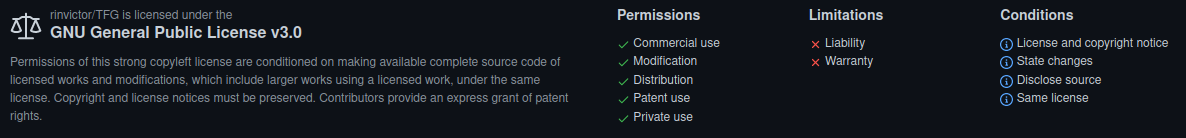
\includegraphics[width=15cm, keepaspectratio]{img/license}
    \caption{Resumen de las condiciones de la licencia GNU General Public License v3.0.}
    \label{figura:license}
\end{figure}

\section{Plan de trabajo}
\label{plan de trabajo}
Las etapas en las que se ha dividido el desarrollo del proyecto para así conseguir los objetivos anteriormente mencionados han sido:

\begin{itemize}
\item \textbf{Estudio previo del tema del TFG}, leyendo diferente literatura sobre automatización y monitorización de jardines e invernaderos.

\item \textbf{Diseño del sistema distribuido a nivel software y hardware}, decidiendo además cuales de los componentes hardware disponibles en el mercado son los más adecuados para la implementación final.

\item \textbf{Iniciación e investigación sobre las tecnologías utilizadas}, por ejemplo, para la aplicación web. Se crearon diferentes programas de prueba para comprender los conceptos básicos del framework utilizado, \textit{Dash}.

\item \textbf{Implementación electrónica de los sensores y desarrollo de los scripts de testeo para estos, recolección de datos y subida a la base de datos de MongoDB}. En primer lugar se implementaron los sensores de humedad y temperatura ambiente y una vez se comprobó el correcto funcionamiento del sistema, se añadieron los de humedad y temperatura de la tierra.

\item \textbf{Desarrollo de la aplicación web}. Permite visualizar la información recogida por los sensores y crear figuras a partir de esta.

\item \textbf{Desarrollo del bot de Telegram}. Permitiendo obtener datos en tiempo real. También se implementó una funcionalidad que permitiese solicitar información concreta a la base de datos, generando resultados textuales y en forma de gráfica.

\item \textbf{Inclusión de los actuadores en el sistema y desarrollo de los scripts de automatización del invernadero}. Añadiendo, además, soporte para los actuadores en la aplicación web y en el bot de Telegram.

\item \textbf{Añadir mayor soporte para el control de errores creando scripts capaces de notificar al usuario vía Telegram sobre estos}. A pesar de que las etapas están claramente diferenciadas, en todos los puntos se ha ido mejorando el control de errores y resolviendo \textit{bugs} que se pudieran detectar. 

\end{itemize}
  
%%%%%%%%%%%%%%%%%%%%%%%%%%%%%%%%%%%%%%%%%%%%%%%%%%%%%%%%%%%%%%%%%%%%%%%%%%%%%%%%
%%%%%%%%%%%%%%%%%%%%%%%%%%%%%%%%%%%%%%%%%%%%%%%%%%%%%%%%%%%%%%%%%%%%%%%%%%%%%%%%
% HERRAMIENTAS %
%%%%%%%%%%%%%%%%%%%%%%%%%%%%%%%%%%%%%%%%%%%%%%%%%%%%%%%%%%%%%%%%%%%%%%%%%%%%%%%%

\cleardoublepage % empezamos en página impar
\chapter{Herramientas} 
\label{chap:herramientas}

En este capítulo se  describen de las distintas herramientas utilizadas para este TFG. Las diferentes tecnologías que se mostrarán en este capítulo se pueden dividir en hardware, incluyendo tanto los sensores y actuadores como la Raspberry pi y el Arduino, y software. En este último, se concretarán las herramientas principales de desarrollo así como las utilizadas para el almacenamiento de los datos recogidos por los sensores.


\section{Hardware}
\label{sec:hardware}

A continuación se presenta el hardware utilizado, todas estas tecnologías son de bajo coste, y entre las múltiples posibilidades existentes en el mercado se han elegido las siguientes para abaratar el presupuesto necesario para realizar este TFG.

\subsection{Raspberry Pi}
\label{subsec:raspberry pi}

Para el desarrollo del TFG se ha utilizado una Raspberry Pi modelo 3B+ (ver figura~\ref{figura:raspberry}). Se trata de un ordenador de placa única concebido por la fundación británica Raspberry Pi Foundation y cuyo primer modelo fue lanzado el 29 de febrero de 2012. En primera instancia, este microcomputador fue desarrollado para acercar la programación y la informática al ámbito educativo. Rápidamente alcanzó una gran popularidad y gracias a la buena acogida está altamente extendido para múltiples proyectos de diferente índole, entre estos proyectos destacan diferentes campos como pueden ser el de la robótica, IoT o la domótica.

Algunas de las principales características de la Raspberry Pi 3 Model B+ son:

\begin{itemize}
	\item Procesador BroadcomBCM2837B0, Cortex-A53(ARMv8) 64-bit SoC
	
	\item Frecuencia de reloj de 1,4 GHz.
	
	\item Memoria RAM de 1 GB LPDDR2 SDRAM.
	
	\item Bluetooth 4.2 BLE

	\item Wi-Fi Dual Band b/g/n/ac
	
	\item Gigabit Ethernet
	
	\item Header GPIO 40 pines.
	
	\item Cuatro puertos USB 2.0, puerto de cámara CSI, puerto de visualización DSI y puerto HDMI
\end{itemize}

Estas características, junto a su ajustado precio, han sido motivo para elegir este modelo.

\begin{figure}[H]
	\centering
    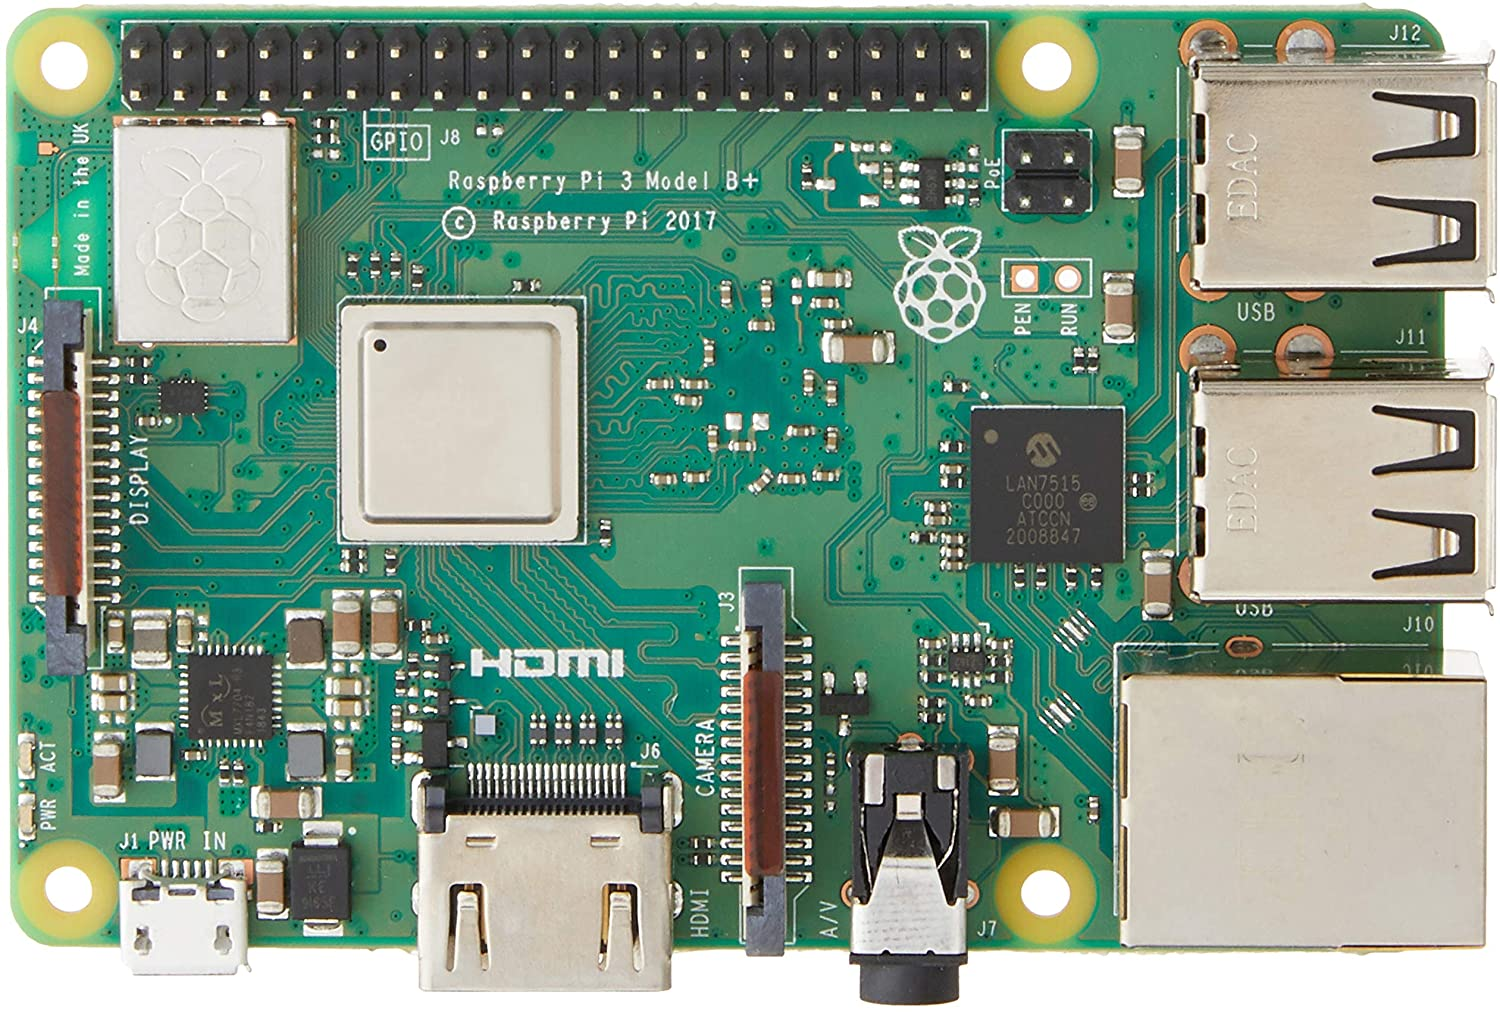
\includegraphics[width=8cm, keepaspectratio]{img/Raspberry}
    \caption{Raspberry Pi 3B+.}
    \label{figura:raspberry}
\end{figure}

La Raspberry Pi posee una serie de entradas y salidas, como se muestra en la figura~\ref{figura:conexiones_raspberry}. A lo largo del desarrollo de la memoria se utiliza la nomenclatura BCM que es la utilizada por el procesador de la Raspberry (ver figura~\ref{figura:pines_raspberry}). Como se puede apreciar, la placa tiene un total de 40 pines GPIO con diferentes propósitos entre los que destacan pines con entradas de 3,3 y 5V, pines a tierra y pines de propósito de general (GPIO).

\begin{figure}[H]
	\centering
    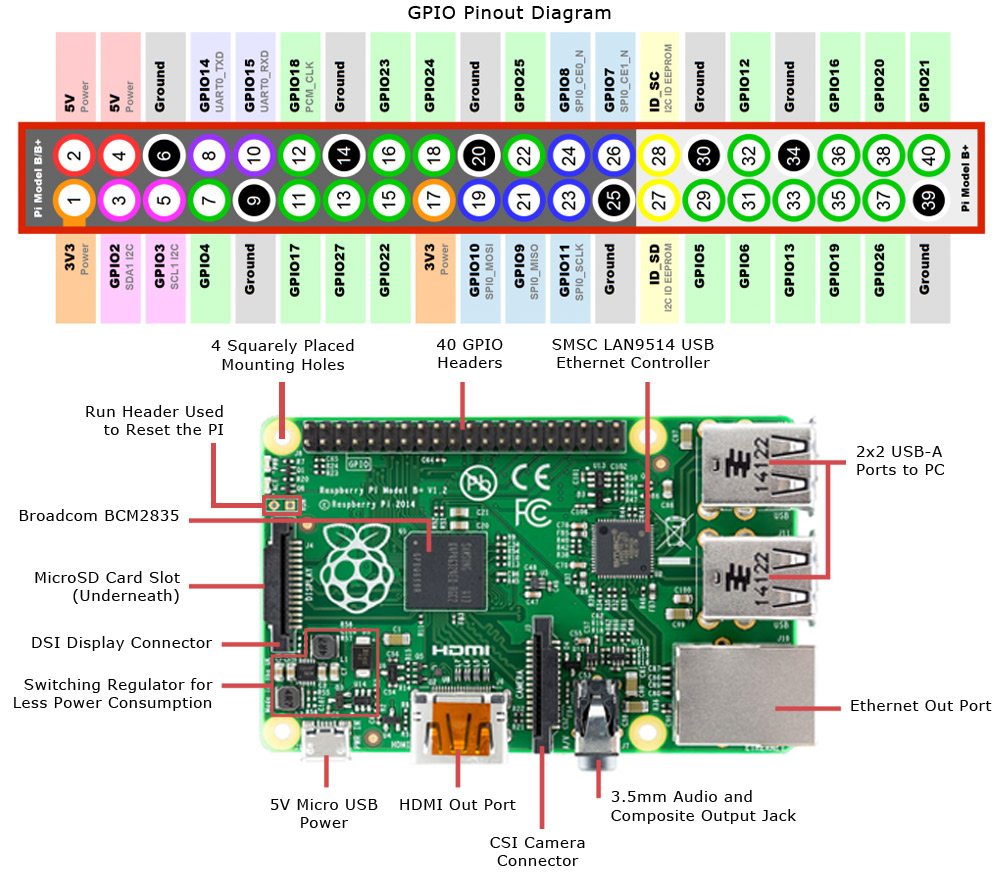
\includegraphics[width=8cm, keepaspectratio]{img/conexiones_raspberry}
    \caption{Diagrama de conexiones de Raspberry Pi Model 3B+.}
    \label{figura:conexiones_raspberry}
\end{figure}


\begin{figure}[H]
	\centering
    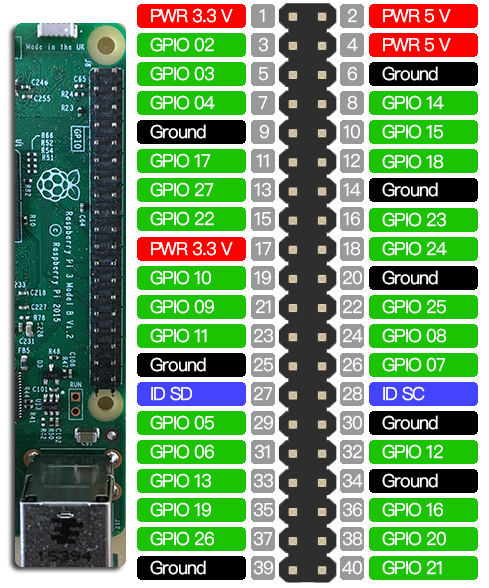
\includegraphics[width=8cm, keepaspectratio]{img/pines_raspberry}
    \caption{Diagrama de pines de Raspberry Pi Model 3B+.}
    \label{figura:pines_raspberry}
\end{figure}

\subsection{Arduino}
\label{subsec:arduino}

Arduino es un proyecto de software libre que, así como el de Raspberry Pi, también fue desarrollado con fines educativos. Está basado en diferentes placas con un microcontrolador. Para trabajar con Arduino se suele utilizar un entorno de programación específico para dichas placas. El lenguaje de programación que se suele utilizar es una adaptación de C++, un lenguaje orientado a objetos, de alto nivel y multiparadigma, pero en este caso se ha utilizado la librería Pyfirmata2, que implementa el protocolo para microcontroladores Firmata. Dicha librería permite interactuar con la placa Arduino usando Python, lenguaje de programación con el que se ha desarrollado la mayoría de este TFG y que se indica en la sección software.

Se ha utilizado la placa Arduino UNO rev3 (ver figura~\ref{figura:arduino}), cuyas principales características son:

\begin{itemize}
	\item Microcontrolador ATmega328P.
	
	\item Funcionamiento a 5V.
	
	\item Voltaje de entrada de 6 a 20V.
	
	\item 14 pines digitales, 6 de ellos con salida PWM.

	\item 6 pines de entrada analógica.
\end{itemize}

De nuevo su precio ha sido motivo para la elección de este modelo de microcontrolador.

\begin{figure}[H]
	\centering
    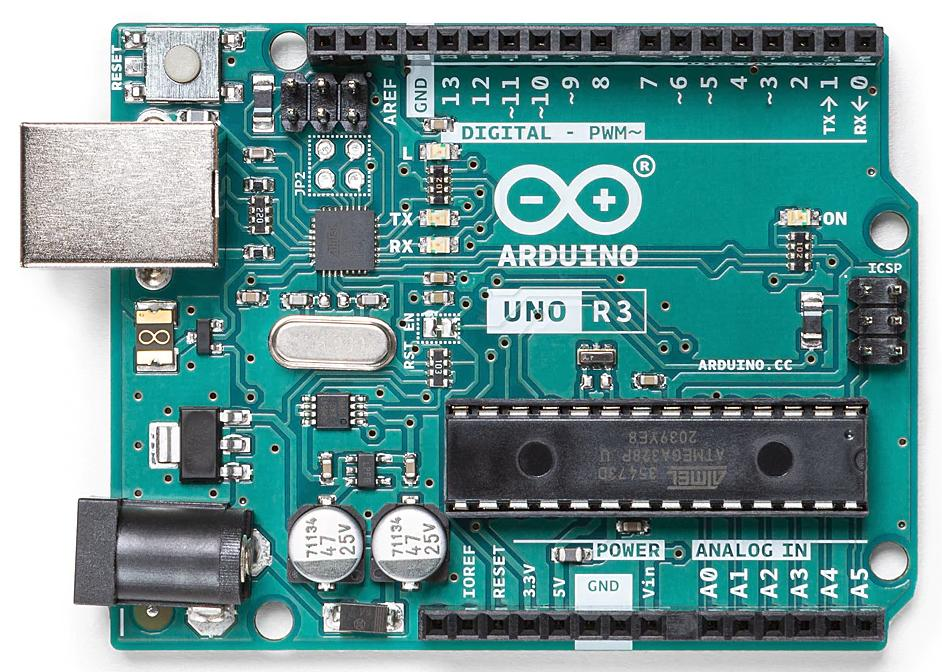
\includegraphics[width=8cm, keepaspectratio]{img/arduino}
    \caption{Arduino UNO rev3.}
    \label{figura:arduino}
\end{figure}

Las diferentes conexiones disponibles en la placa Arduino se muestran en la figura~\ref{figura:conexiones_arduino}

\begin{figure}[H]
	\centering
    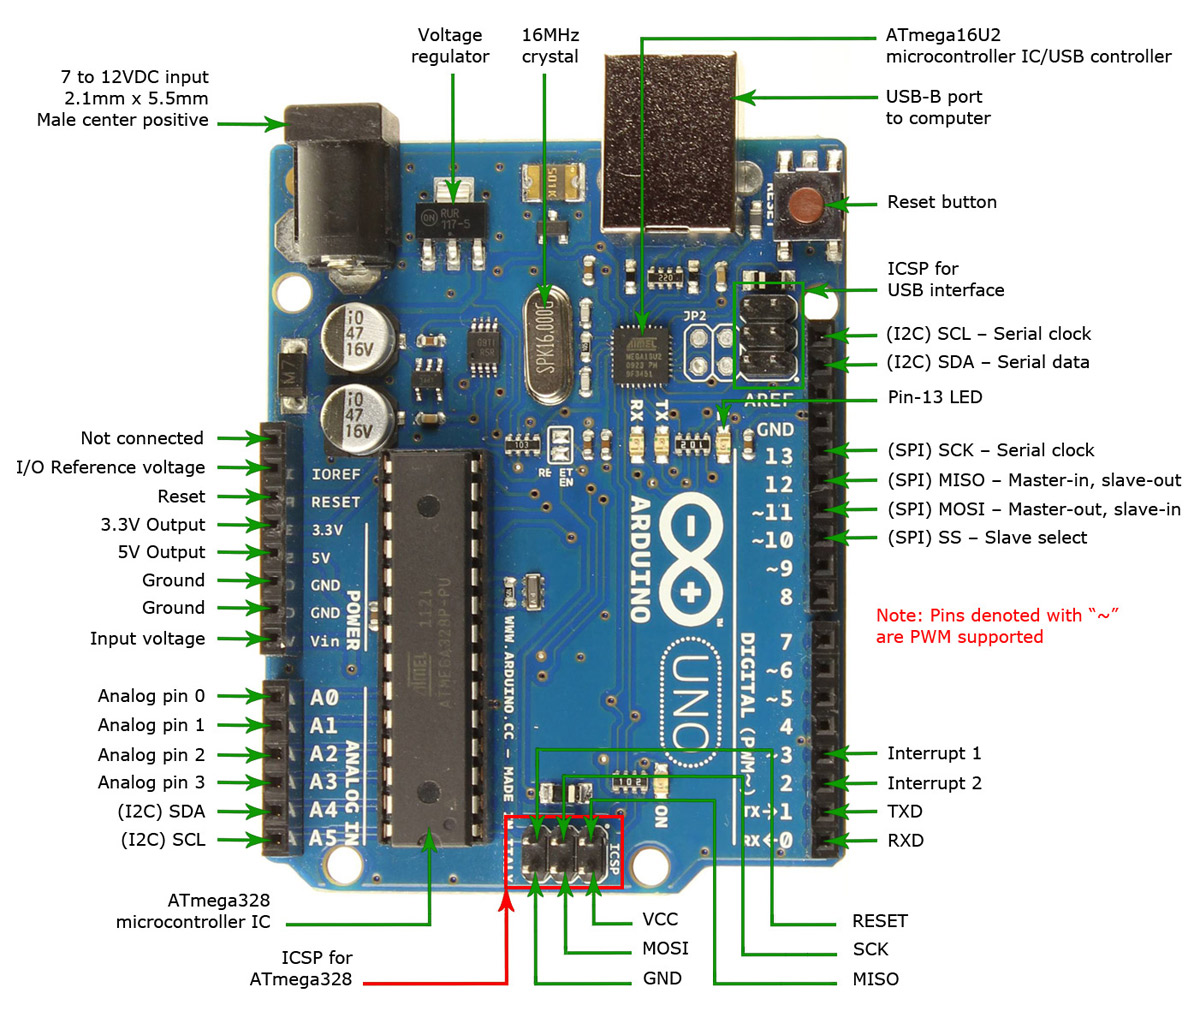
\includegraphics[width=8cm, keepaspectratio]{img/conexiones_arduino}
    \caption{Diagrama de conexiones y pines de Arduino UNO rev3.}
    \label{figura:conexiones_arduino}
\end{figure}

\subsection{Sensores}
\label{subsec:sensores}

Se han usado diferentes tipos de sensores para medir las principales magnitudes que afectarán al cuidado y a la monitorización de las plantas del invernadero. Estas magnitudes son temperatura y humedad ambiente, temperatura de la tierra y humedad de la tierra. Para realizar estas mediciones se ha utilizado el módulo \textit{DHT22} para temperatura y humedad ambiente, una sonda \textit{DS18B20} para la temperatura de la tierra y un módulo \textit{YL-69} para la humedad de la tierra.

En sus fichas técnicas podemos destacar diferentes características que son especialmente relevantes para cada uno de los sensores mencionados anteriormente:

\begin{itemize}
	\item Sensor DHT22:
	\begin{itemize}
		\item 3-5V de entrada/salida.
		\item Rango de temperaturas de -40 a 80 ºC. Con una precisión de ±0.5 ºC
		\item Lectura de humedad en un rango de 0-100\%. Con una precisión de ±5 puntos porcentuales.
		\item Tasa de muestreo de 0.5 Hz.
	\end{itemize}
\end{itemize}

\begin{itemize}
	\item Sensor DS18B20:
	\begin{itemize}
		\item 3-5.5V de entrada/salida.
		\item Rango de temperaturas de -55 a 125 ºC. Con una precisión de ±0.5 ºC
		\item Tasa de muestreo de 1.3 Hz.
	\end{itemize}
\end{itemize}

\begin{itemize}
	\item Sensor YL-69:
	\begin{itemize}
		\item 2-6V de entrada/salida.
		\item Lectura de humedad analógica. Con una precisión del 5-10\%.
		\item Tasa de muestreo de 0,5 Hz.
	\end{itemize}
\end{itemize}

\begin{figure}[H]
  \centering
  \begin{minipage}[b]{0.4\textwidth}
    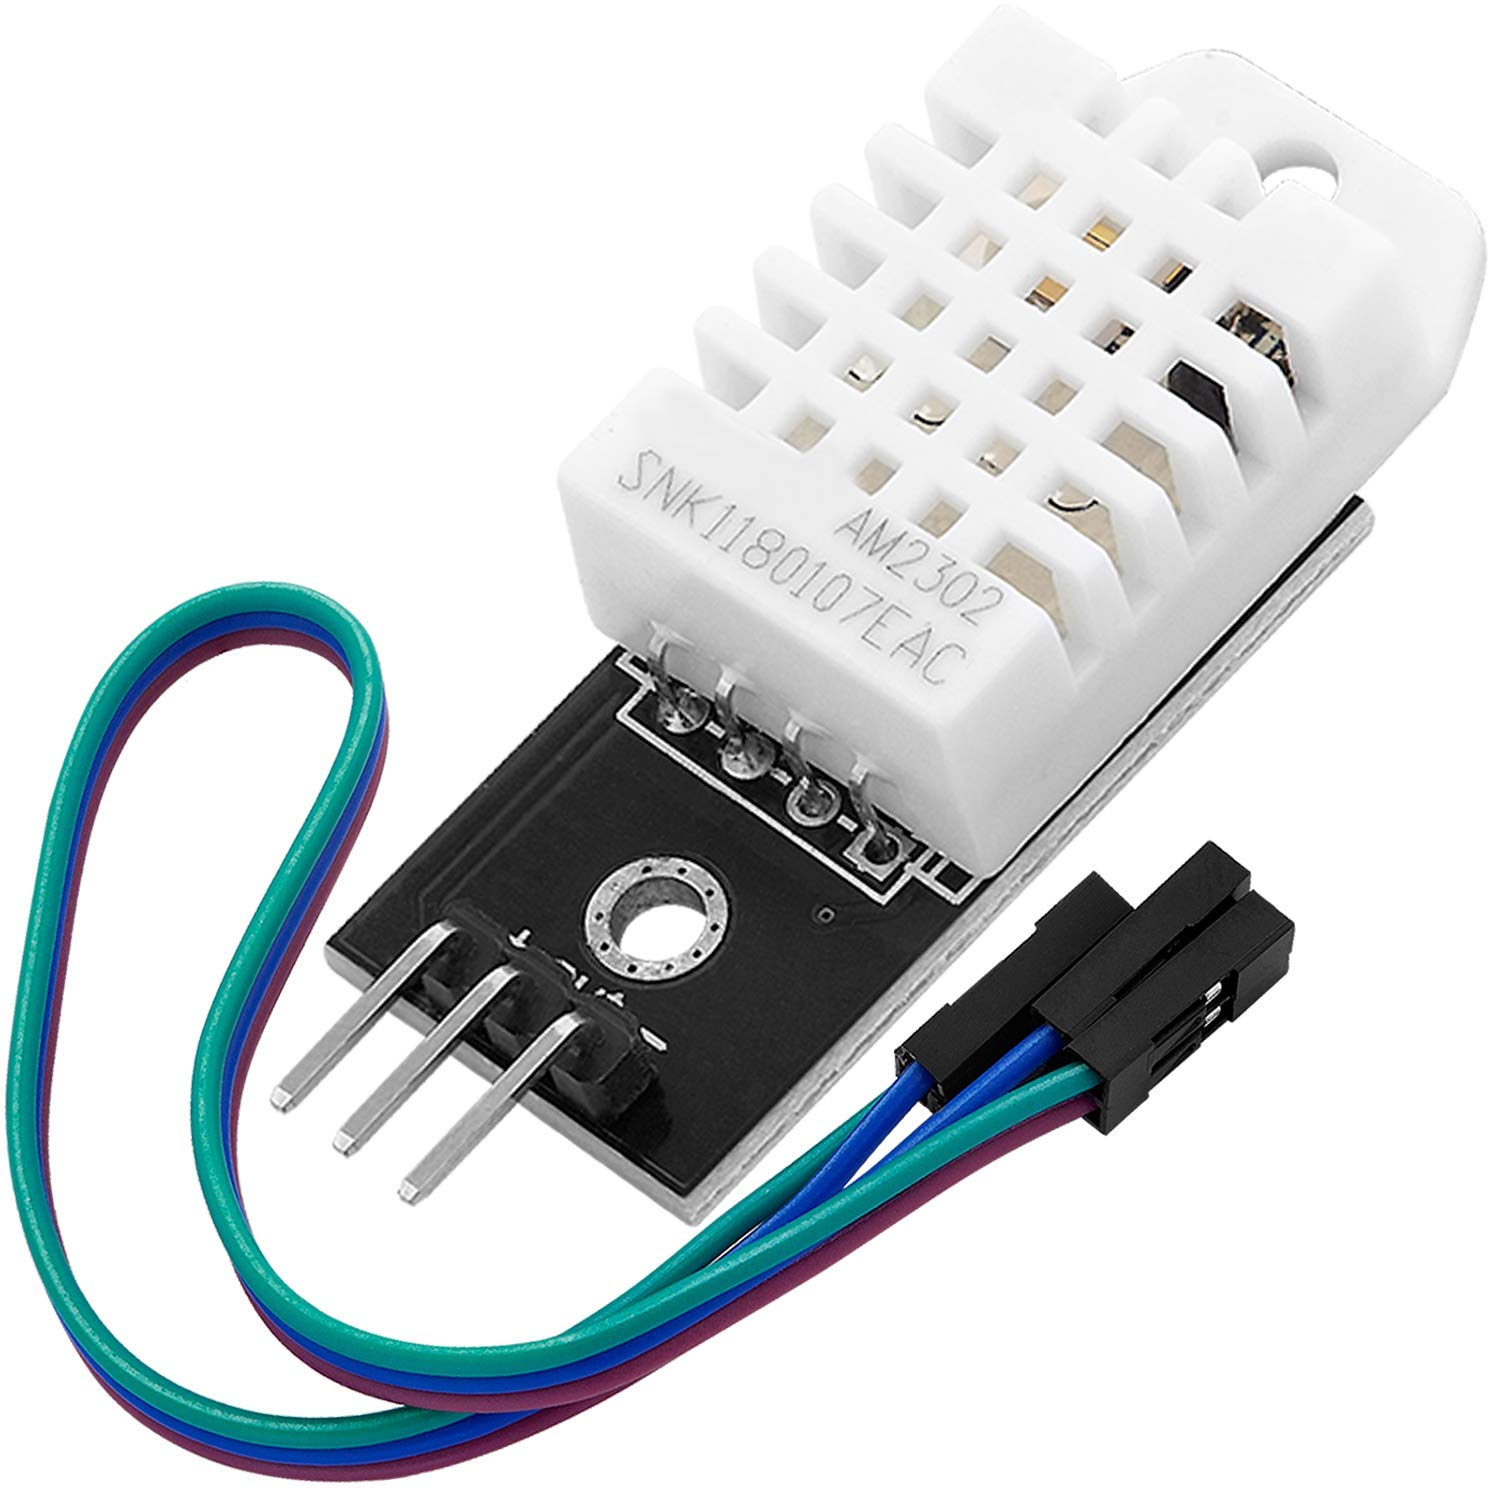
\includegraphics[width=\textwidth]{img/dht22}
    \caption{Módulo DHT22.}
    \label{figura:modulo_dht22}
  \end{minipage}
  \hfill
  \begin{minipage}[b]{0.4\textwidth}
    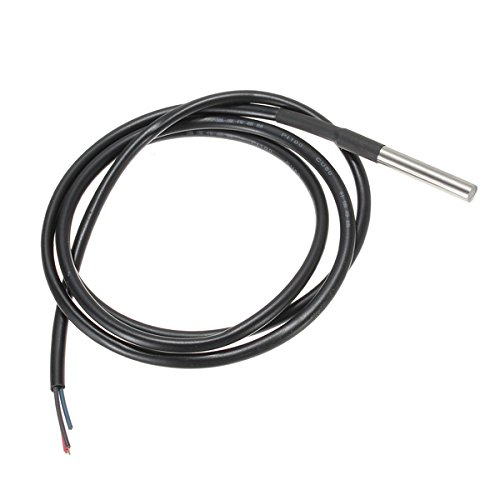
\includegraphics[width=\textwidth]{img/ds18b20}
    \caption{Sonda DS18B20.}
    \label{figura:sonda_ds18b20}
  \end{minipage}
  \hfill
    \begin{minipage}[b]{0.4\textwidth}
    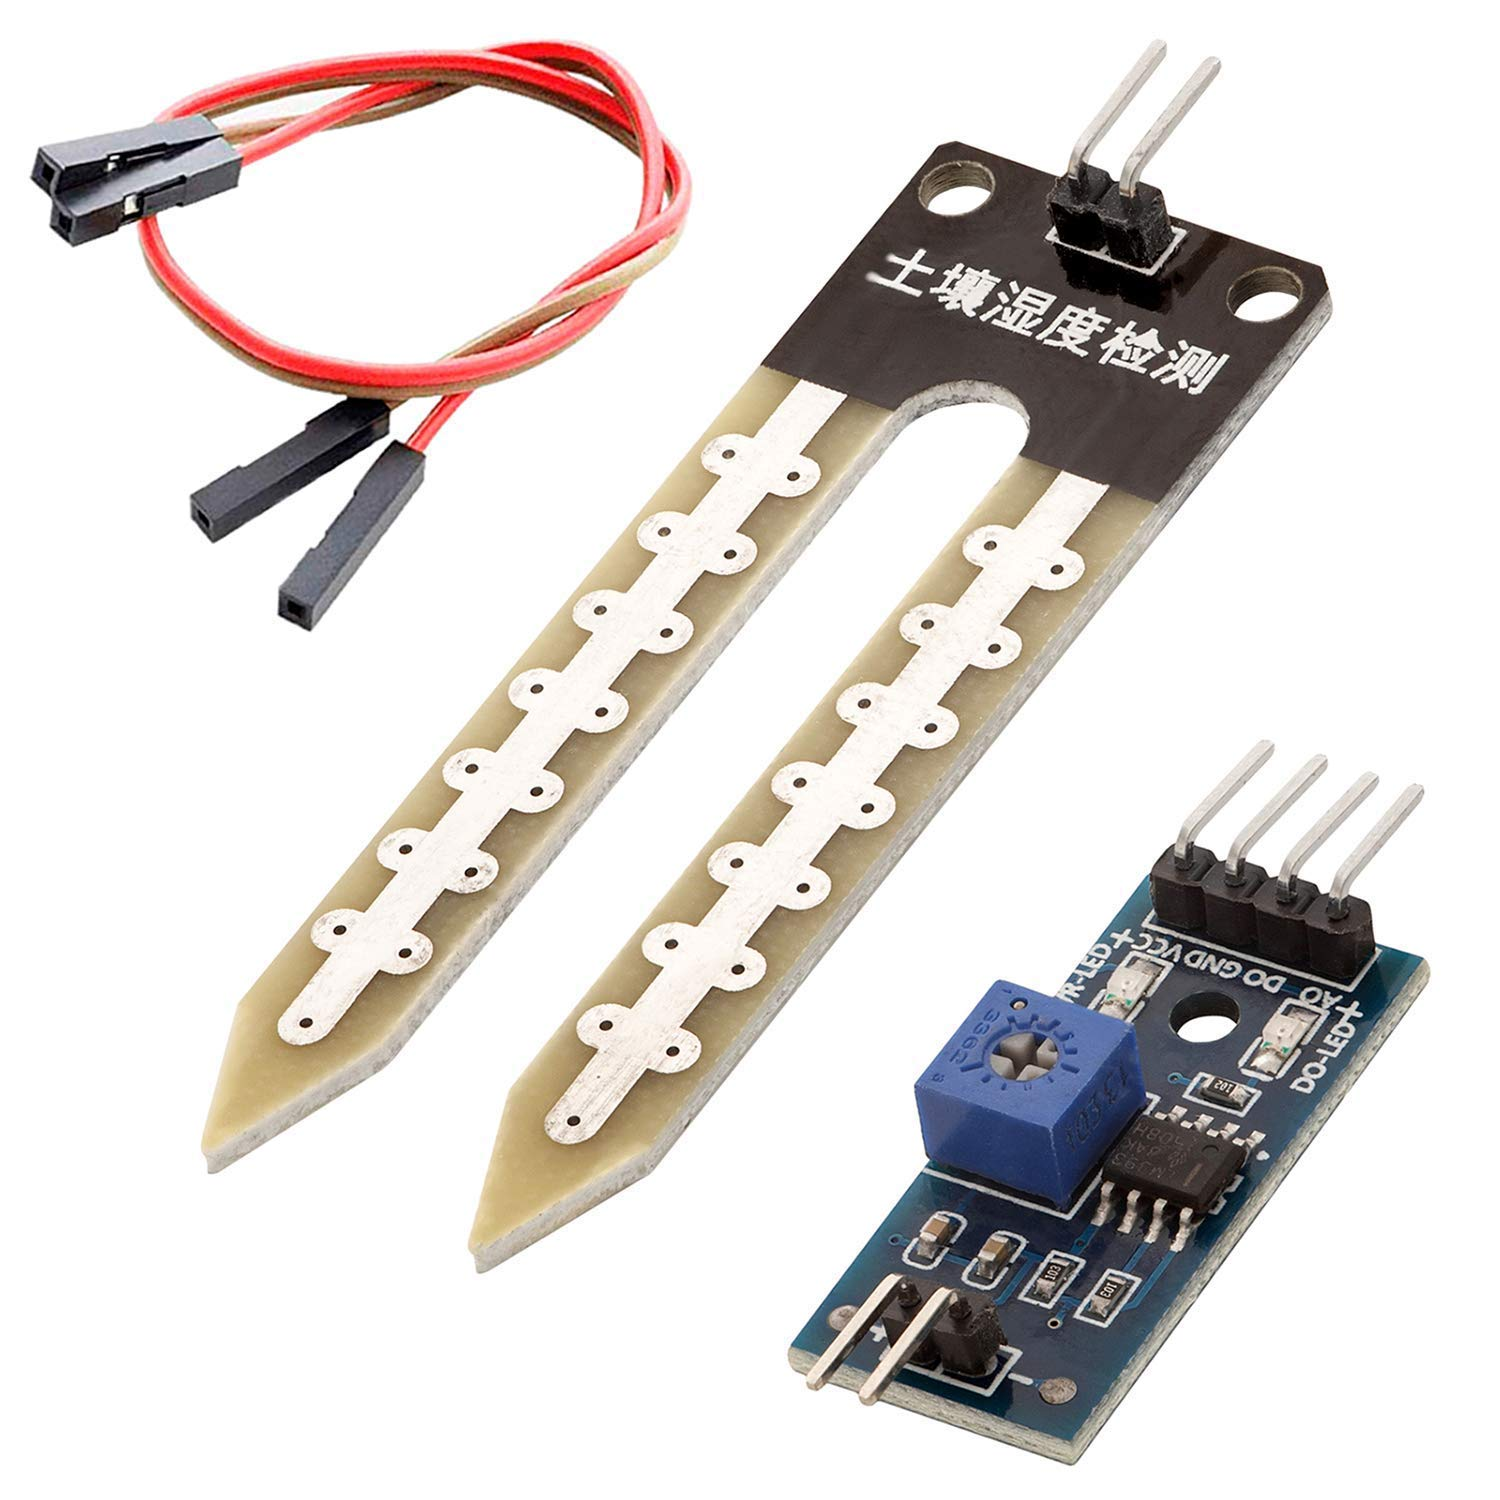
\includegraphics[width=\textwidth]{img/yl-69}
    \caption{Módulo YL-69.}
    \label{figura:yl_69}
  \end{minipage}
\end{figure}

\subsection{Actuadores}
\label{subsec:actuadores}

Los actuadores son útiles en cualquier proyecto de IoT, pues utilizando la información obtenida por los sensores, permiten desarrollar sistemas complejos basados en toma de decisiones e interactuar con el medio. 
En este TFG se ha implementado un sistema de riego automático basado en la humedad de la tierra. Tal y como se indica en la sección~\ref{sec:trabajos futuros}, se podría usar esta información proporcionada por los sensores para incluir nuevas funcionalidades en el sistema y automatizar diferentes tareas.

Para el funcionamiento del sistema de riego se ha usado una bomba de agua modelo CESFONJER, funciona a 12V DC, tiene una potencia de levantamiento de agua de hasta 3 metros y un caudal de 250L/h.

Se ha añadido al sistema electrónico un módulo de 8 relés, cuyo propósito es el de poder controlar la bomba, que funciona a 12V y está conectada a la corriente eléctrica. El tener un módulo de 8 relés proporciona la posibilidad de añadir diferentes actuadores para trabajos futuros como motores, bombas de agua o luces.

\begin{figure}[H]
  \centering
  \begin{minipage}[b]{0.4\textwidth}
    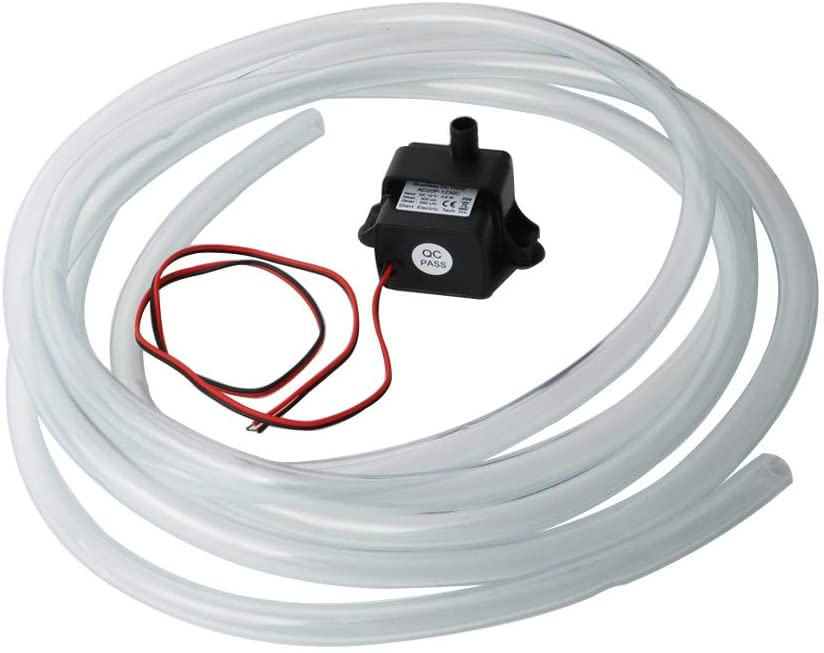
\includegraphics[width=\textwidth]{img/bomba_cesfonjer}
    \caption{Bomba de agua modelo CESFONJER.}
    \label{figura:bomba_cesfonjer}
  \end{minipage}
  \hfill
  \begin{minipage}[b]{0.4\textwidth}
    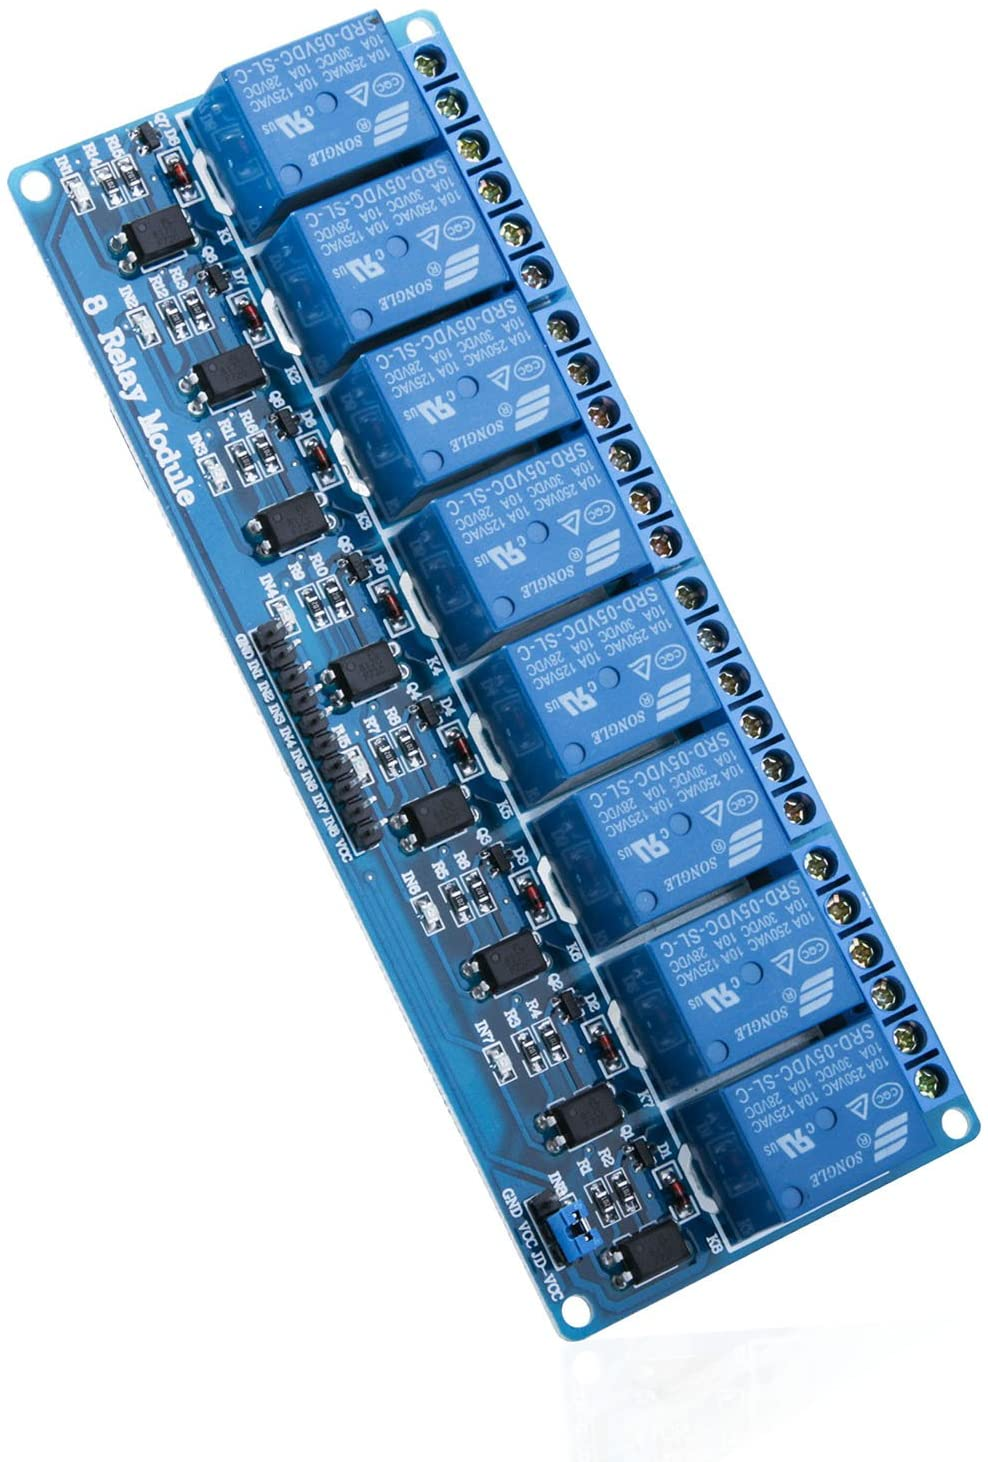
\includegraphics[width=\textwidth]{img/reles}
    \caption{Módulo de relés.}
    \label{figura:reles}
  \end{minipage}
\end{figure}
 

\section{Software}
\label{software}
En esta sección se presentan las diferentes herramientas software utilizadas para el desarrollo del proyecto. Todas estas son gratuitas.

\subsection{Raspbian}
\label{subsec:raspbian}
Raspberry Pi OS, popularmente conocido como Raspbian, es una distribución de GNU/Linux, y es el sistema operativo típicamente utilizado en cualquier modelo de Raspberry. Desde 2015 se proporciona de forma oficial como el sistema operativo por defecto para estas placas.
Se trata de un SO libre y tiene, tal y como cualquier distribución GNU/Linux, multitud de posibilidades.
Toda la funcionalidad de la Raspberry para este TFG se ha implementado sobre Raspbian.

\subsection{Python}
\label{subsec:python}
Python es un lenguaje de programación de alto nivel, interpretado, multiplataforma, de código abierto y de propósito general. Una de sus grandes ventajas es la sencillez y la legibilidad a la hora de desarrollar aplicaciones usando este lenguaje, además, de la multitud de librerías y frameworks disponibles. Soporta no solo la programación orientada a objetos sino también la programación imperativa y la funcional.
Fue desarrollado a finales de la década de los 80 por Guido Van Rossum, investigador del centro holandés Centrum Wiskunde \& Informatica.
Su uso está hoy en día ampliamente extendido. Es muy común en diferentes áreas de la ciencia y la ingeniería y es uno de los lenguajes de programación más solicitados en el mercado.
En este TFG se han usado dos versiones diferentes de Python, la Python 3.8 y la 3.5, debido al soporte de las diferentes librerías.
Los principales módulos utilizados se irán referenciando a lo largo de la siguiente sección.

\subsection{Bash}
\label{subsec:bash}
GNU Bash (Bourne-again shell), popularmente conocido como Bash es un intérprete de comandos propio de GNU/Linux.
Bash scripting consiste en utilizar Bash como un lenguaje de programación usando las instrucciones propias de este intérprete. Cuando se habla de Bash scripting se habla de un tipo de Shell Scripting propio de los sistemas GNU/Linux, existen muchos otros, no solo para Linux, sino para cualquier sistema operativo como pueden ser Cmd.exe, Csh, AppleScript, COMMAND.COM, ect. En este TFG se ha utilizado Bash para realizar scripts que lanzan diferentes procesos, como el de la recolección de datos a partir de los sensores, por ejemplo.

\subsection{Dash}
\label{subsec:dash}

Dash es un framework de código abierto utilizado para desarrollar aplicaciones de visualización de datos interactivas usando Python, R, Julia o F\#. Está escrito sobre Plotly.js y React.js. Las aplicaciones web creadas con Dash son servidores web Flask, un framework escrito en Python para crear aplicaciones web, que se comunican usando JSON, un formato ligero para intercambiar datos, sobre HTTP (Hypertext Transfer Protocol).
El front-end Dash está implementado con React.js, una librería de JavaScript para la interfaz de usuario escrita y mantenida por Facebook. Dash, además de las diferentes tecnologías citadas anteriormente, tiene integrados HTML y CSS. En este TFG se ha usado, también, Bootstrap, que se explica a continuación y Plotly, una librería de Python utilizada para crear gráficos interactivos. Dash ha sido utilizado para desarrollar una aplicación web que permite visualizar gráficas de los datos almacenados en la base de datos de MongoDB.

\subsubsection{HTML en Dash}
\label{subsubsec:html}
HTML (HyperText Markup Language), es un lenguaje de marcado para la elaboración de páginas web. Actualmente, es un estándar en Internet a cargo de W3C (World Wide Web Consortium).
El origen de HTML data de principios de la década de los 80, fue creado por Tim-Berners Lee, físico en el CERN (European Organization for Nuclear Research), como un sistema para poder compartir documentos de manera más sencilla a la utilizada hasta el momento. A lo largo de los años se ha ido actualizando e incluyendo multitud de mejoras, actualmente se utiliza HTML5, lanzado en el año 2005.
El uso de HTML en Dash se realiza mediante la librería Dash.html, que incluye todos los elementos de HTML, a continuación podemos ver un breve ejemplo de uso extraído de su documentación oficial y de su equivalencia en HTML clásico:

\begin{lstlisting}[language=Python]
from dash import html

html.Div([
    html.H1('Hello Dash'),
    html.Div([
        html.P('Dash converts Python classes into HTML'),
        html.P("This conversion happens behind the scenes by Dash's JavaScript front-end")
    ])
])
\end{lstlisting}

\begin{lstlisting}[language=HTML]
<div>
    <h1>Hello Dash</h1>
    <div>
        <p>Dash converts Python classes into HTML</p>
        <p>This conversion happens behind the scenes by Dash's JavaScript front-end</p>
    </div>
</div>
\end{lstlisting}


\subsubsection{CSS en Dash}
\label{subsubsec:css}
Las hojas de estilo en cascada, CSS(Cascading Style Sheets), son empleadas para dar estilo a un documento escrito con un lenguaje de marcado como puede ser HTML, fue desarrollado por W3C en 1996. Hoy en día la relación entre CSS y HTML es muy alta, de hecho, CSS es también un estándar en Internet y en el diseño web. En Dash también existe la posibilidad de dar estilo usando CSS, para el desarrollo de esta aplicación se ha utilizado Bootstrap 5.

\begin{figure}[H]
  \centering
  \begin{minipage}[b]{0.4\textwidth}
    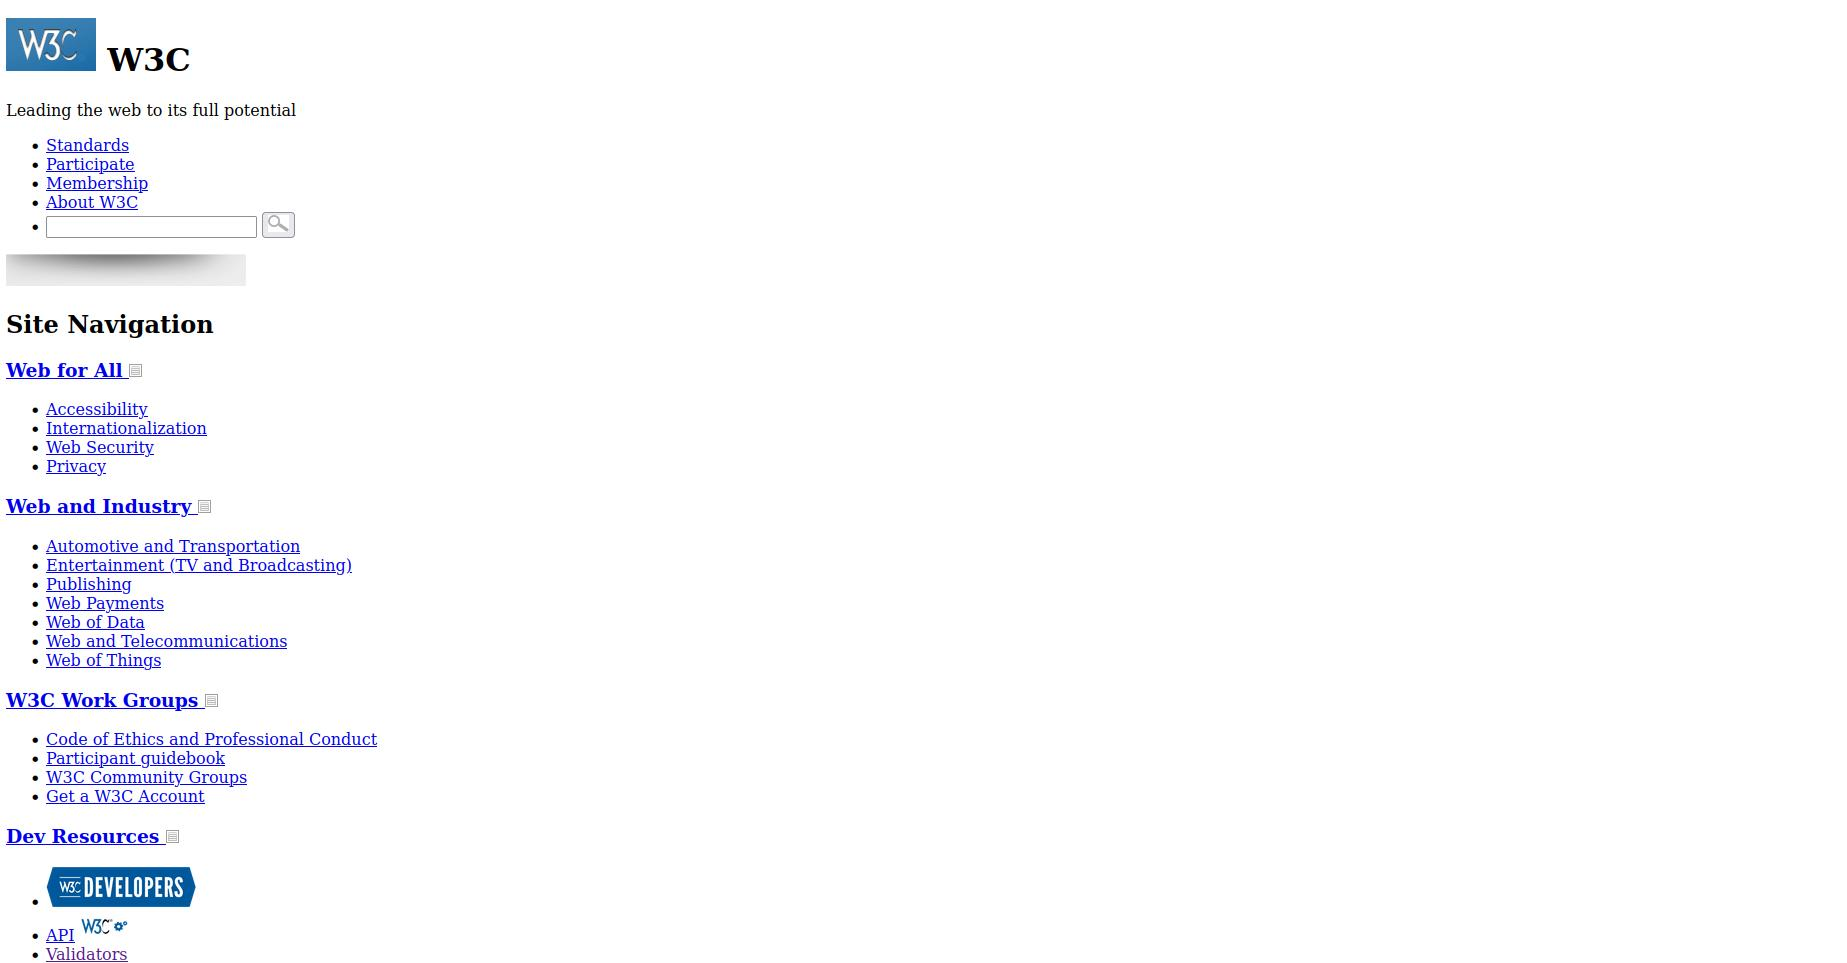
\includegraphics[width=\textwidth]{img/w3c_sin_css}
    \caption{Página de ejemplo sin estilo.}
    \label{figura:w3c_sin_css}
  \end{minipage}
  \hfill
  \begin{minipage}[b]{0.4\textwidth}
    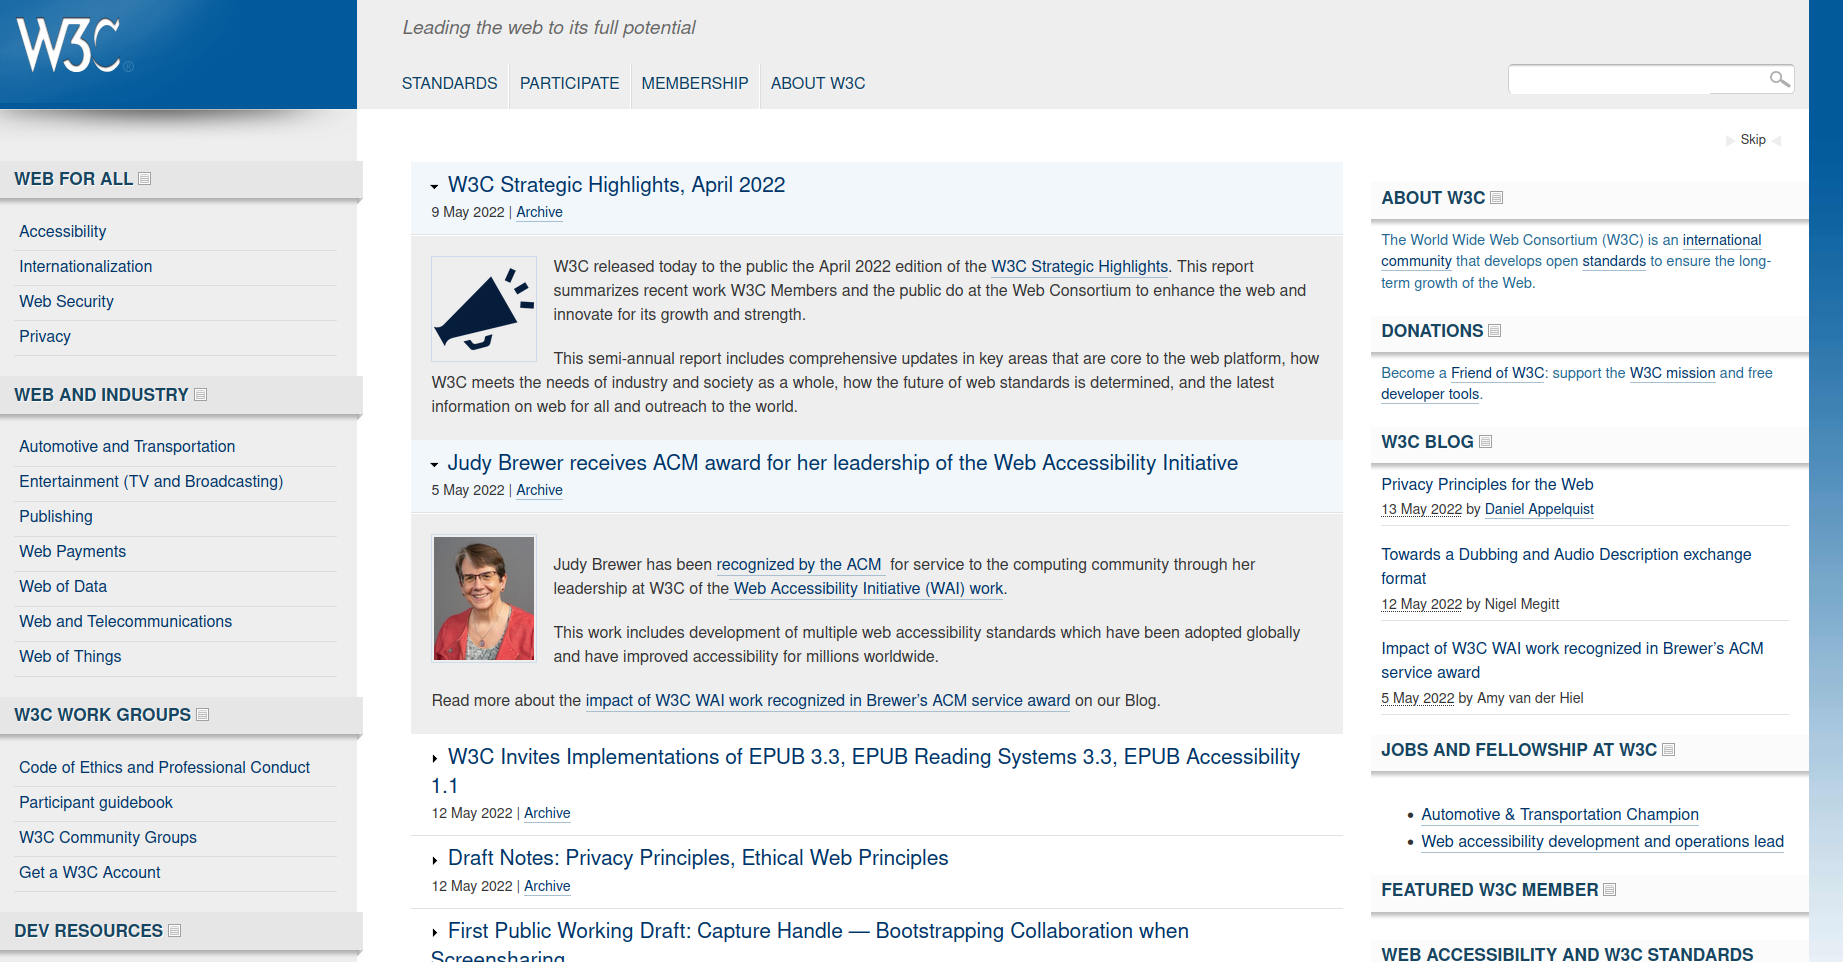
\includegraphics[width=\textwidth]{img/w3c_con_css}
    \caption{Página de ejemplo con estilo CSS.}
    \label{figura:w3c_con_css}
  \end{minipage}
\end{figure}

\subsubsection{Bootstrap en Dash}
\label{subsubsec:boostrap}
Este framework de software libre, muy utilizado en programación web, se utiliza como una abstracción de HTML, CSS y JavaScript. Su propósito es facilitar la creación de sitios web para múltiples dispositivos (\textit{responsive design}). Fue desarrollado inicialmente en el año 2011 por ingenieros de la compañía estadounidense Twitter, Inc. Su versión más reciente es Bootstrap 5, lanzada en el año 2021, cuya principal diferencia respecto a sus anteriores versiones es que se basa en Vanilla JavaScript (JavaScript puro), en lugar de JQuery, una librería de JavaScript muy utilizada para agregar interactividad a los sitios web.
Como se ha mencionado anteriormente, se ha usado una plantilla libre de Bootstrap 5 a la que se le han hecho ligeras modificaciones de estilo, se puede trabajar con este framework en Dash mediante la librería Dash\_bootstrap\_components.

\subsection{API de telegram}
\label{subsec:api telegram}

Una API (Application Programming Interfaces) o interfaz de programación de aplicaciones en español, es un conjunto de protocolos y definiciones que se utilizan para desarrollar software y con las que se pueden comunicar dos aplicaciones. Telegram es una aplicación de mensajería instantánea desarrollada por los hermanos Nikilái y Pável Dúrov, lanzada el 14 de agosto de 2013. Telegram permite multitud de servicios, entre ellos la posibilidad de utilizar bots. Los bots de telegram tienen una gran popularidad y con muy diferentes usos, con ellos se puede desde obtener información hasta realizar descargas o traducir textos.

Telegram ofrece una API para la creación de bots, que es la que se ha utilizado en este TFG junto al módulo Telepot para Python para desarrollar un bot que permite visualizar datos de manera gráfica y textual.

\subsection{MongoDB}
\label{subsec:mongodb}

MongoDB es un sistema de bases de datos de código abierto, no relacional y orientado a documentos. Utiliza estructuras BSON (Binary JSON) para guardar los datos. Una de las principales ventajas de MongoDB es su velocidad y aprovechamiento de los recursos.

Las bases de datos no relacionales son elegidas para muchos proyectos de IoT y, en general, en proyectos para los que no sea necesario guardar relaciones entre tablas al estilo SQL (Structured Query Language). MongoDB permite acceder a una gran cantidad de datos en poco tiempo, realizar multitud de consultas, expresiones regulares, etc.

Es habitual trabajar con Python y MongoDB, para ello se ha usado la librería Pymongo, es una de las más extendidas para este propósito y está en continuo desarrollo. El propósito en este TFG de MongoDB ha sido almacenar información recogida por los sensores e información sobre las acciones tomadas por los actuadores.

\subsection{Cron}
\label{subsec: cron}
Se ha usado Cron para administrar diferentes tareas. Cron es un demonio (administrador regular de procesos en segundo plano) de UNIX. Permite ejecutar procesos y tareas basados en tiempo.
En este TFG se ha usado Cron para lanzar periódicamente scripts para la realización de diferentes tareas como la recolección automática de los datos de los sensores.
 
\subsection{Docker}
\label{subsec: docker}

Docker es un sistema basado en el funcionamiento de virtualización ofrecida por el núcleo de Linux.
Este prepara máquinas virtuales de proceso y usa diferentes tecnologías como Cgroups, que permite aislar y limitar los recursos consumidos por un grupo de procesos o el espacio de nombrado de Linux (Linux kernel namespaces), que permite aislar los PID, interfaces de red, tablas de encaminamiento, puntos de montaje, etc. Docker es un sistema muy extendido y de código abierto mantenido por Docker Inc. Algunos de los principales organismos contribuyentes a este proyecto son Google, Cisco, Microsoft, RedHat, entre otras importantes compañías, además de la comunidad.
En este caso se ha utilizado Docker para realizar el despliegue de la base de datos de MongoDB en una máquina de los laboratorios de la ETSIT de la Universidad Rey Juan Carlos.

\begin{figure}[H]
	\centering
    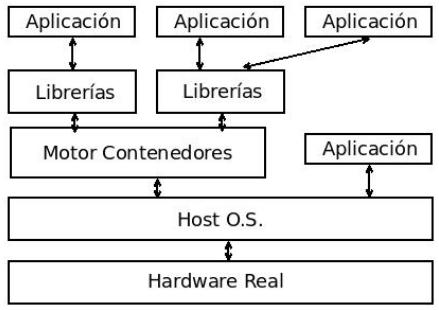
\includegraphics[width=8cm, keepaspectratio]{img/docker}
    \caption{Diagrama simplificado del funcionamiento de la virtualización por contenedores.}
    \label{figura:esquema_docker}
\end{figure}

\subsection{Heroku}
\label{subsec: heroku}
Heroku, fundada en 2007 por Orion Henry, James Lindenbaum y Adam Wigginses y desde 2010 mantenida por Salesforce Inc., es una plataforma de servicios en la nube o PaaS (Platform as a Service), en inglés, que permite manejar la administración y configuración de los servidores.
Las principales características de esta popular herramienta son:
\begin{itemize}
	\item Soporta diferentes lenguajes de programación (Ruby, PHP, Python, etc).
	\item Ofrece diferentes características de seguridad como certificación SSL y autenticación.
	\item Tiene una versión gratuita de manejo sencillo.
\end{itemize}

Para este proyecto se ha utilizado su versión más sencilla para desplegar la aplicación web de visualización de datos desarrollada usando Dash. Existen otras alternativas pero gracias a su facilidad de uso ha sido elegida sobre el resto.


\subsection{Control de versiones}
\label{subsec:control versiones}

El control de versiones es esencial en cualquier proyecto de desarrollo de software, se ha utilizado Git y Github para este propósito.

Git es el sistema de control de versiones más extendido actualmente, se trata de un proyecto de software libre en continuo crecimiento. Desarrollado por Linus Torvalds en el año 2005. Git es un sistema de control de versiones distribuido, de tal manera que cada copia del trabajo es también un repositorio que alberga todo el historial de cambios.

Una de las principales ventajas del uso de Git es su rendimiento, y es que gracias a su popularidad, que lo ha convertido prácticamente en un estándar, las bases de sus características son muy sólidas y sus principales funciones están muy optimizadas. Otro aspecto a resaltar de este software es la seguridad, utiliza SHA1, un algoritmo criptográficamente seguro. Todo esto ha llevado a Git a ser el sistema de control de versiones más usado.
Github es una plataforma diseñada para alojar código, comprada por Microsoft en el año 2018, permite gestionar proyectos usando Git. Es también muy utilizado y permite alojar proyectos tanto de forma pública como privada.

\begin{figure}[H]
	\centering
    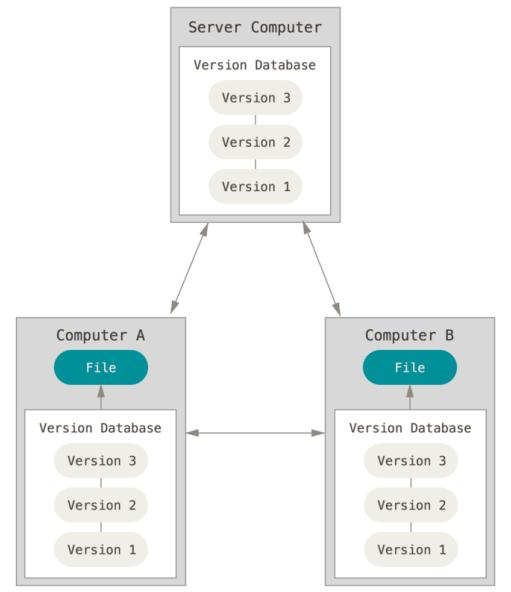
\includegraphics[width=8cm, keepaspectratio]{img/git}
    \caption{Esquema de concepto básico de Git.}
    \label{figura:esquema_git}
\end{figure}

%%%%%%%%%%%%%%%%%%%%%%%%%%%%%%%%%%%%%%%%%%%%%%%%%%%%%%%%%%%%%%%%%%%%%%%%%%%%%%%%
%%%%%%%%%%%%%%%%%%%%%%%%%%%%%%%%%%%%%%%%%%%%%%%%%%%%%%%%%%%%%%%%%%%%%%%%%%%%%%%%
% DISEÑO E IMPLEMENTACIÓN %
%%%%%%%%%%%%%%%%%%%%%%%%%%%%%%%%%%%%%%%%%%%%%%%%%%%%%%%%%%%%%%%%%%%%%%%%%%%%%%%%

\cleardoublepage
\chapter{Diseño e implementación}
\label{chap:diseño e implementación}
En este capítulo se expone la implementación del sistema que se ha llevado a cabo en este TFG. Se detalla cada una de las herramientas que se han desarrollado tanto desde el punto vista de hardware como desde el de software.

\section{Montaje físico del invernadero}
\label{sec: montaje físico del invernadero}
En esta sección se explica el montaje físico del invernadero y se detalla su arquitectura.
El invernadero ha diseñado para ser de bajo coste. Ha sido fabricado en plástico, mide 2.5x1.25x0.75 metros y en su interior se han introducido sacos de cultivo para plantar. Se ha elegido este tipo invernadero ya que se considera adecuado teniendo en cuenta el espacio disponible para su ubicación. En la figura~\ref{figura:invernadero} se muestra el invernadero que se ha montado para el desarrollo de este TFG.
\begin{figure}[H]
	\centering
    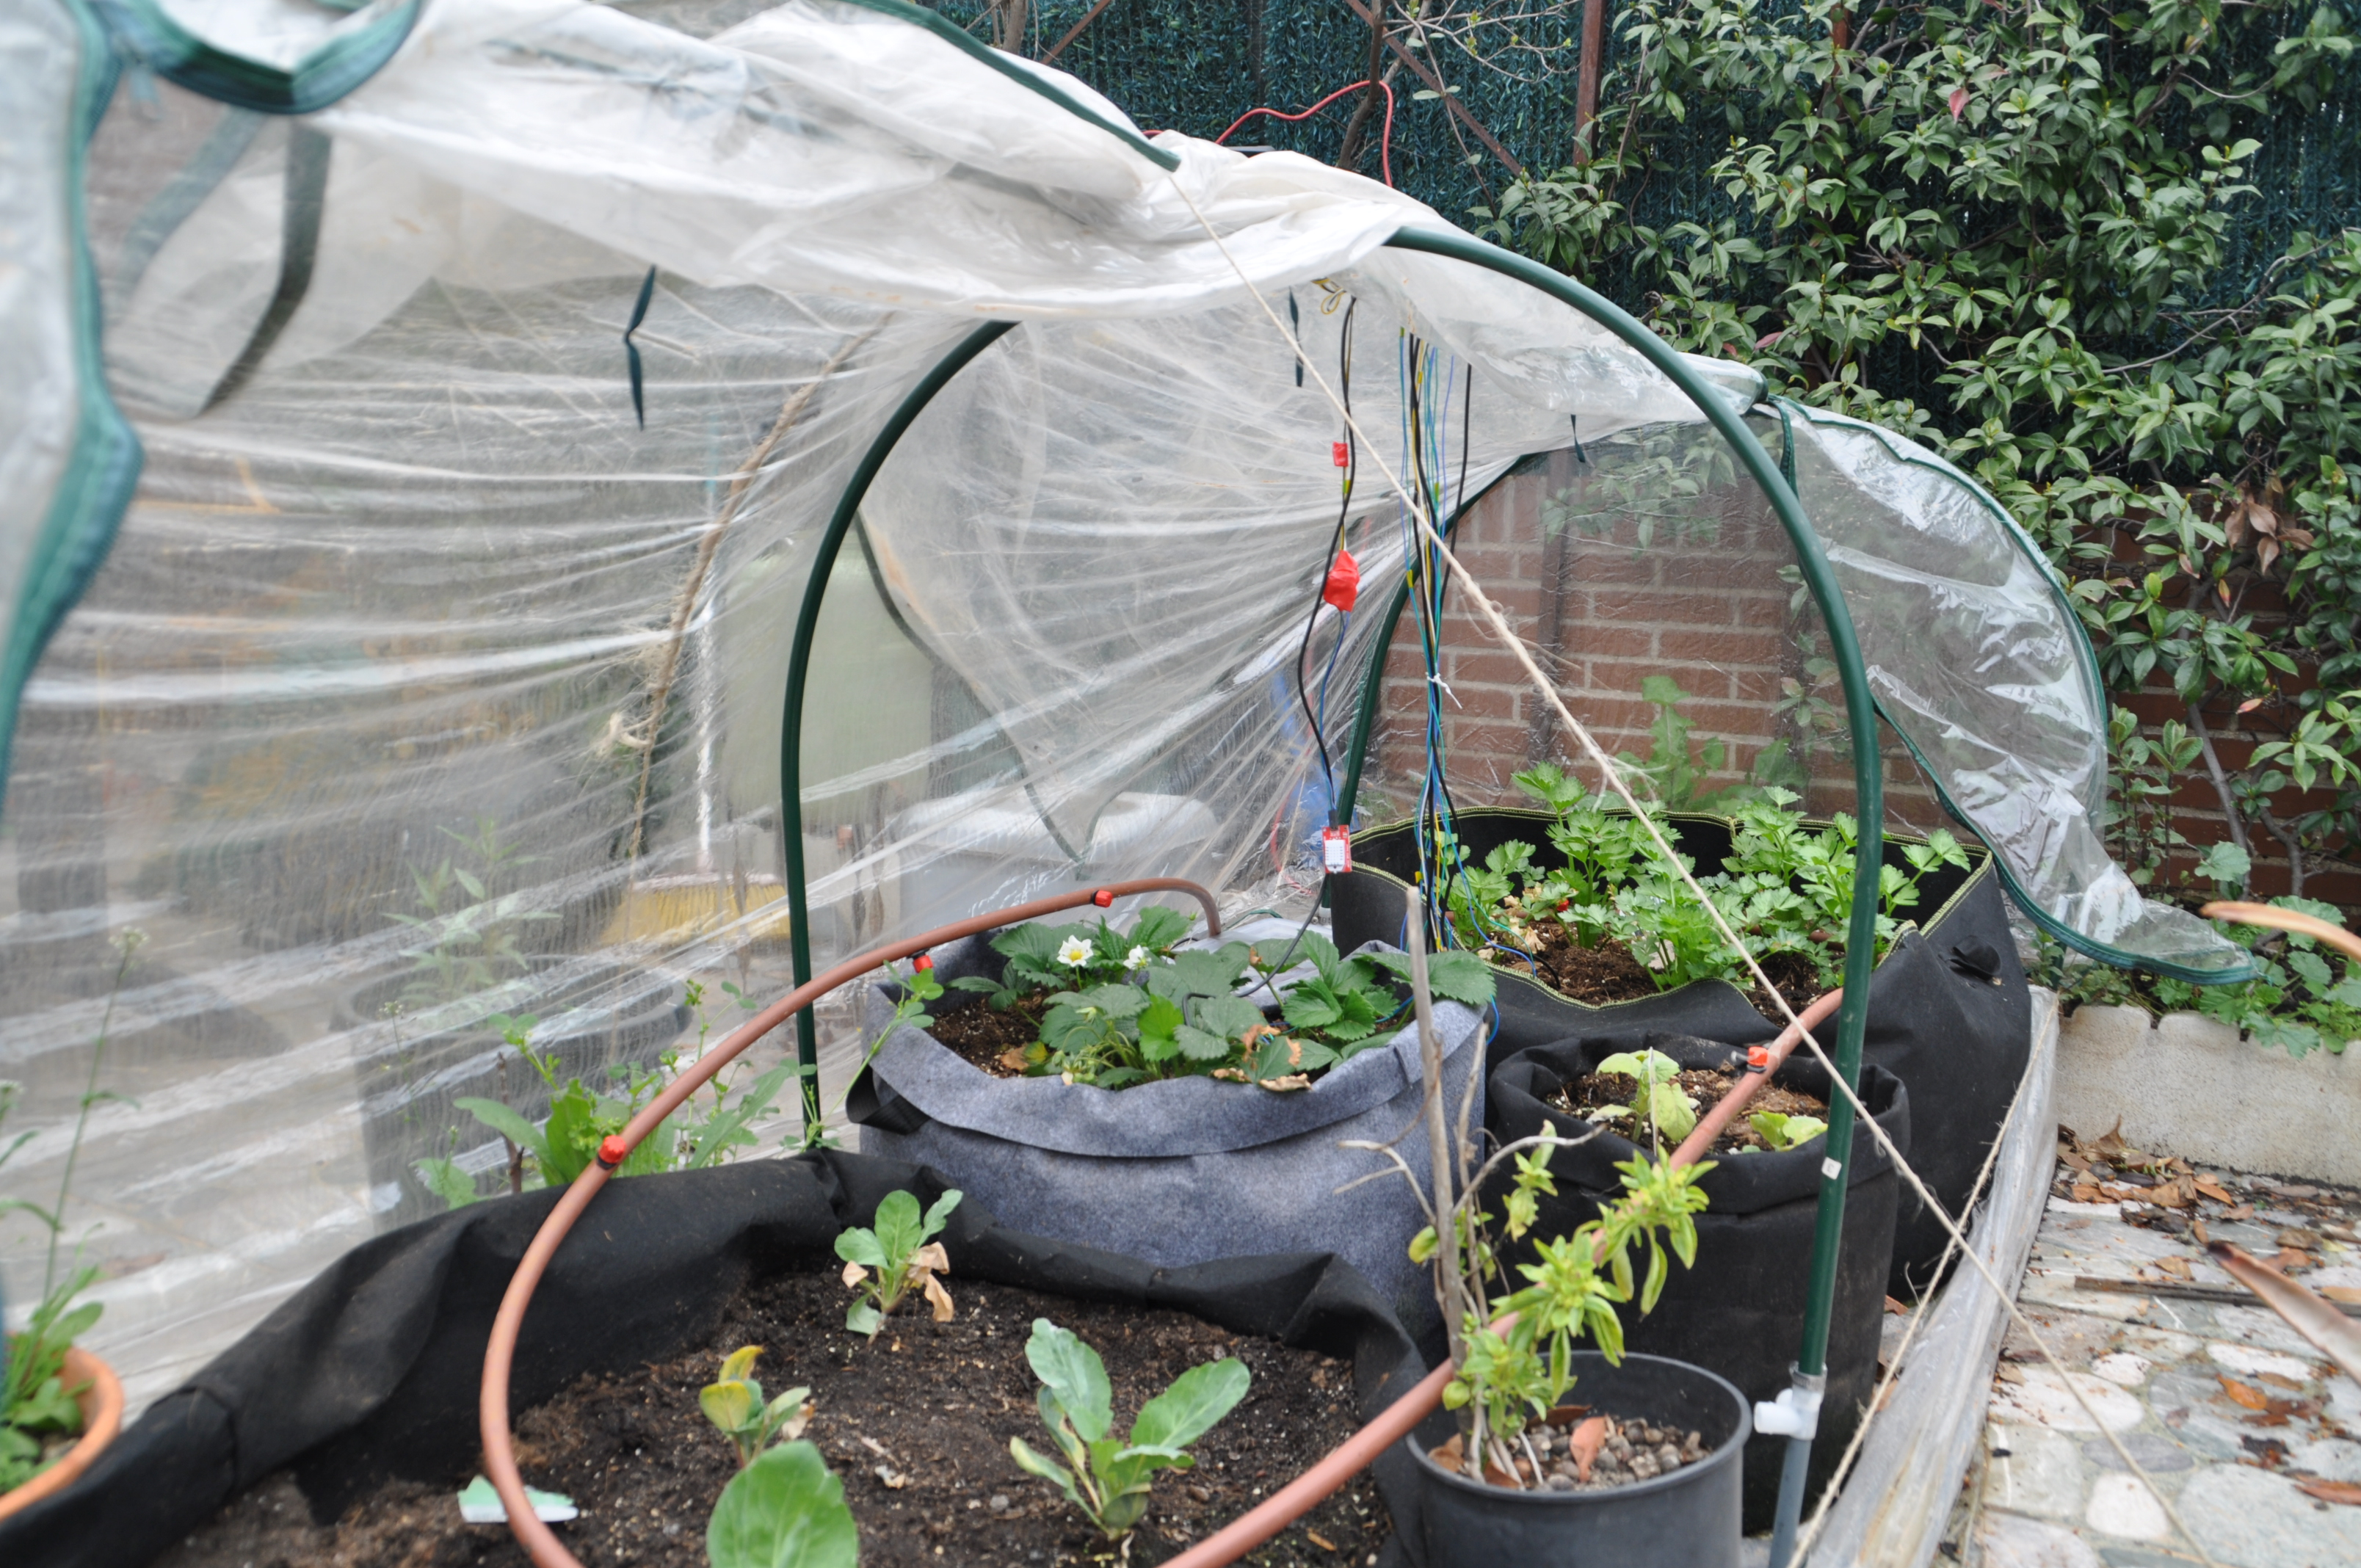
\includegraphics[width=8cm, keepaspectratio]{img/invernadero}
    \caption{Implementación física del invernadero.}
    \label{figura:invernadero}
\end{figure}

En este montaje se ha incluido un depósito de agua. El depósito cuenta con una capacidad de 40 litros, capacidad que permite realizar las pruebas del sistema.  
Otra opción hubiera consistido en utilizar una toma de agua corriente en lugar de un depósito. En el montaje propuesto para este TFG el depósito está desacoplado de una toma de agua, por lo que debe rellenarse manualmente.  Aunque existe en este caso la limitación de acceso al agua, nos permite por otro lado que el invernadero no dependa de infraestructuras externas. Otra opción viable y que no implicaría ningún cambio sería, por ejemplo, sustituir el depósito por un pozo. Para poder llevar el agua hasta las plantas se ha usado una tubería de riego con puntos de salida de agua regulables tipo araña conectado a una bomba como se puede observar en las figuras~\ref{figura:bomba_agua} y~\ref{figura:salidas_agua}. La bomba de agua modelo CESFONJER será el actuador que se controlará mediante el software desarrollado para realizar el riego del sistema.

\begin{figure}[H]
  \centering
  \begin{minipage}[b]{0.4\textwidth}
    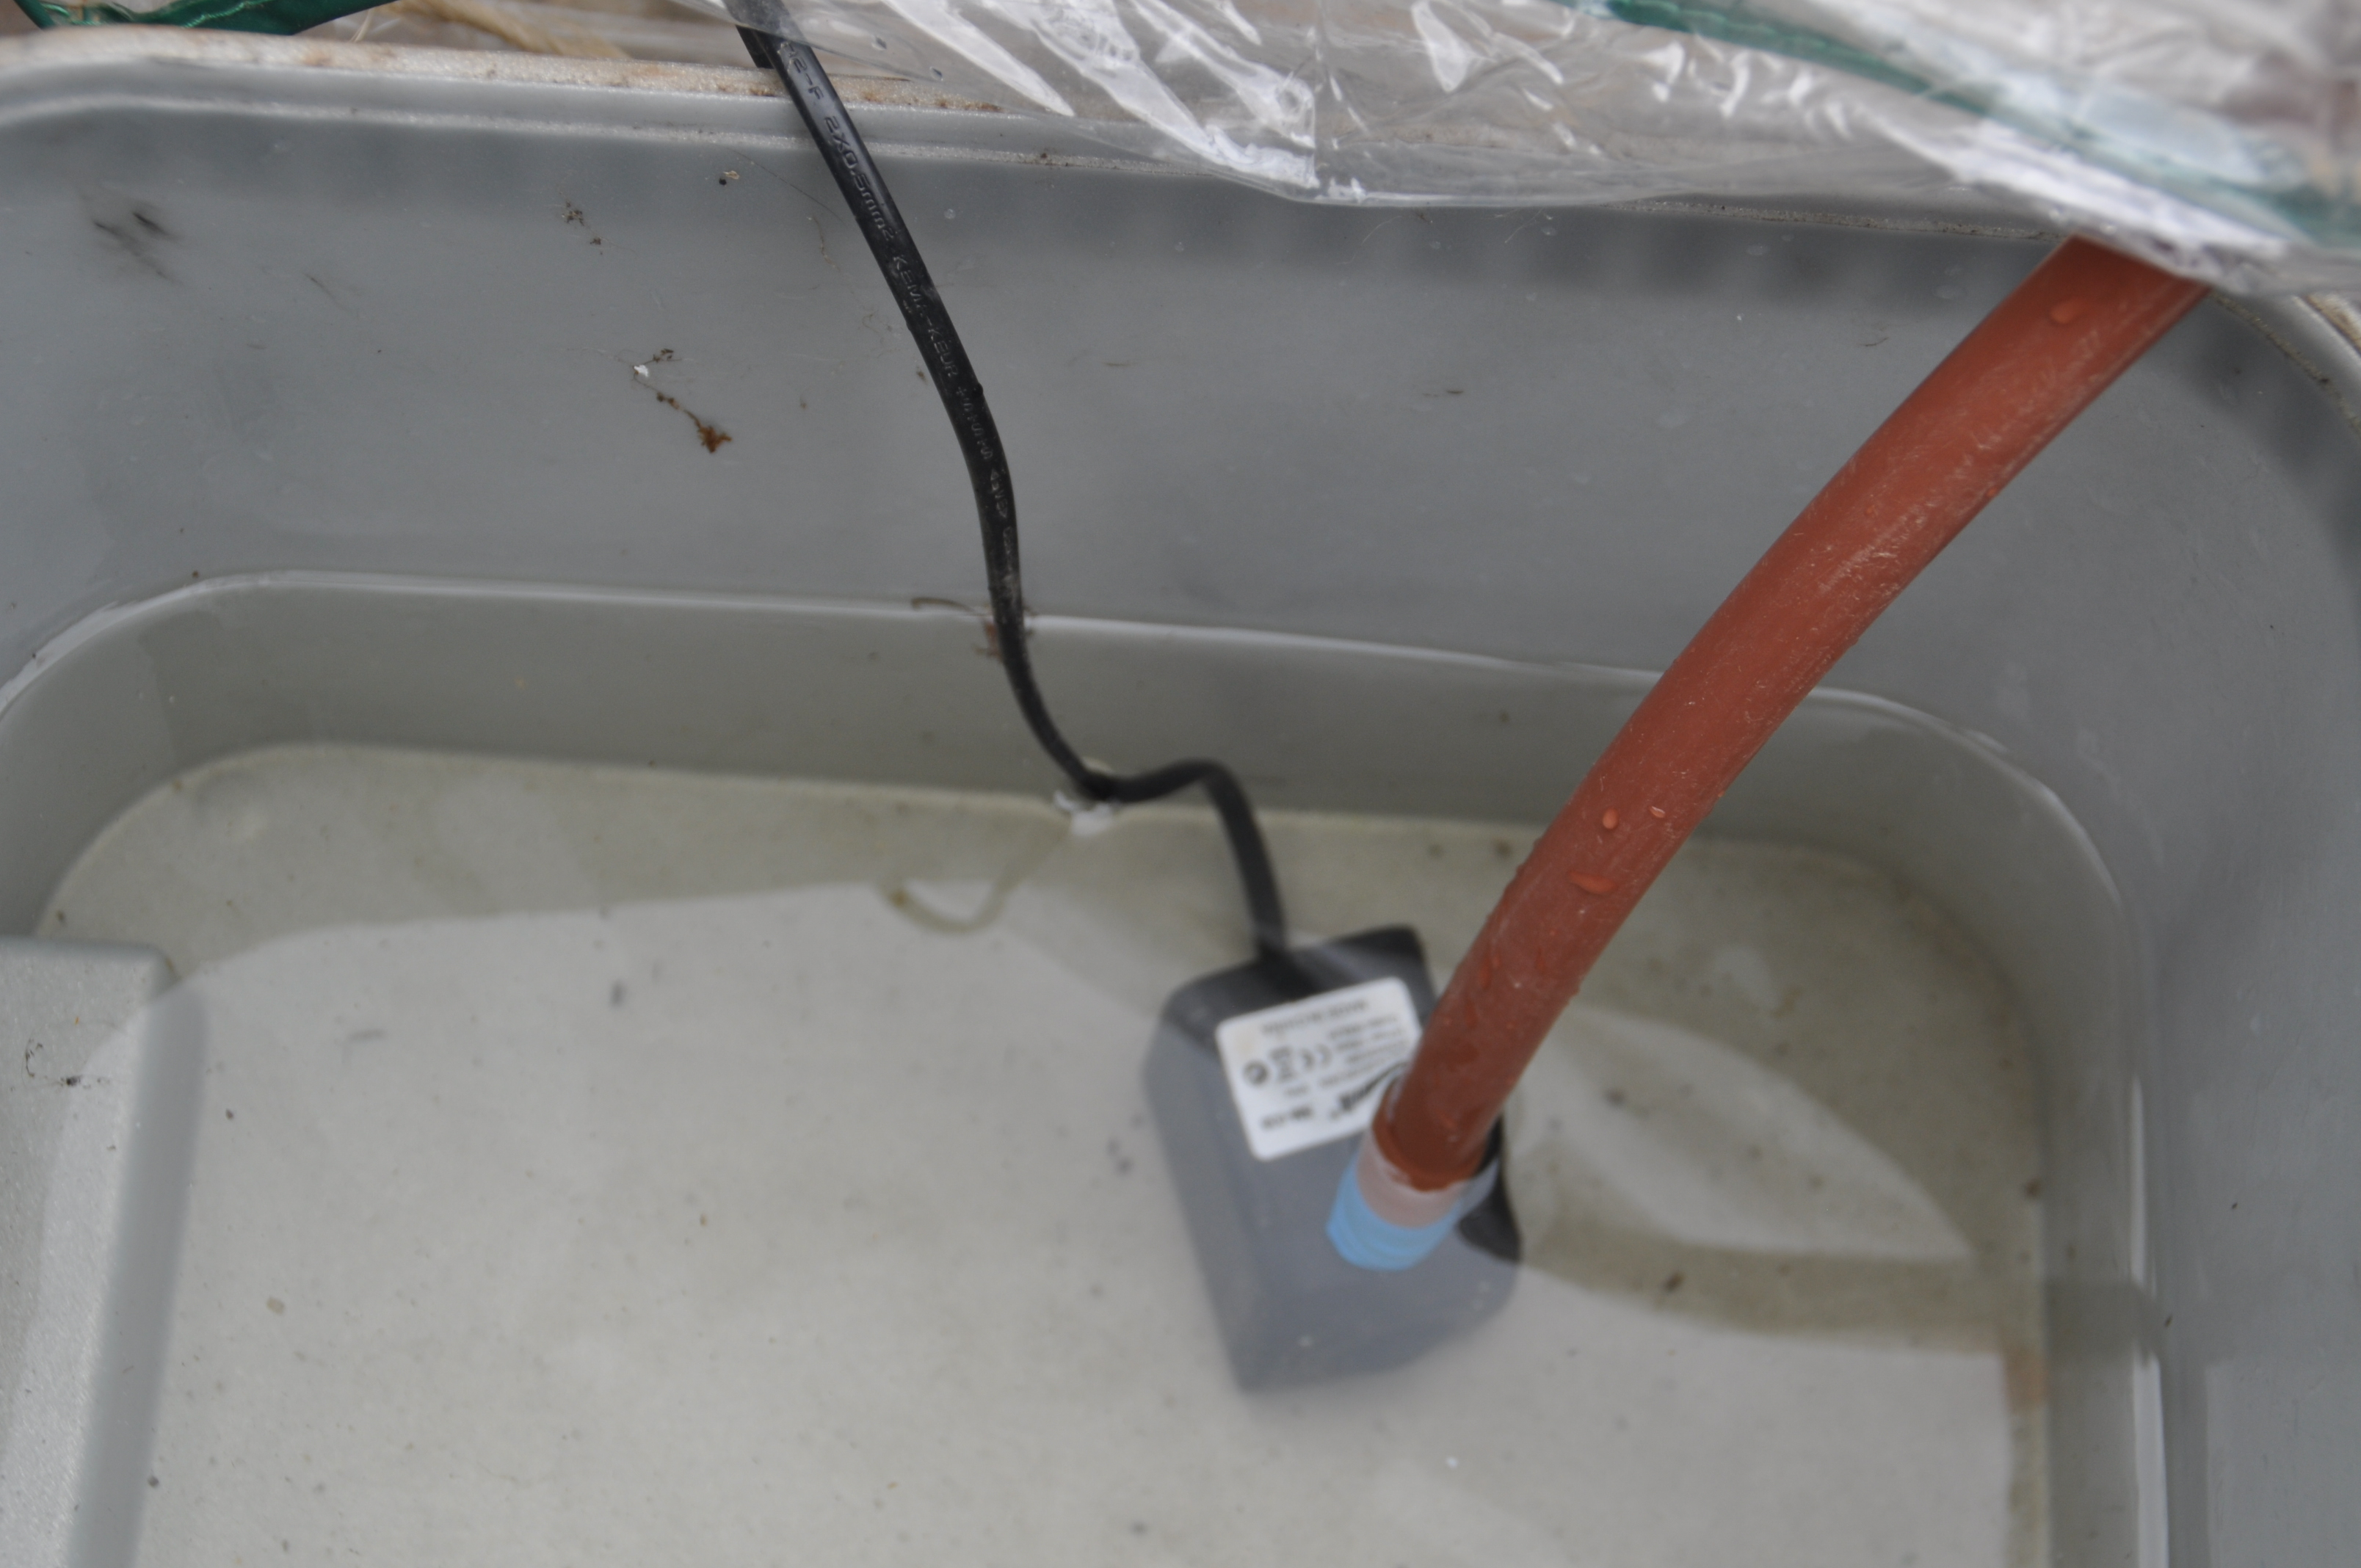
\includegraphics[width=\textwidth]{img/bomba_agua}
    \caption{Bomba de agua en el depósito.}
    \label{figura:bomba_agua}
  \end{minipage}
  \hfill
  \begin{minipage}[b]{0.4\textwidth}
    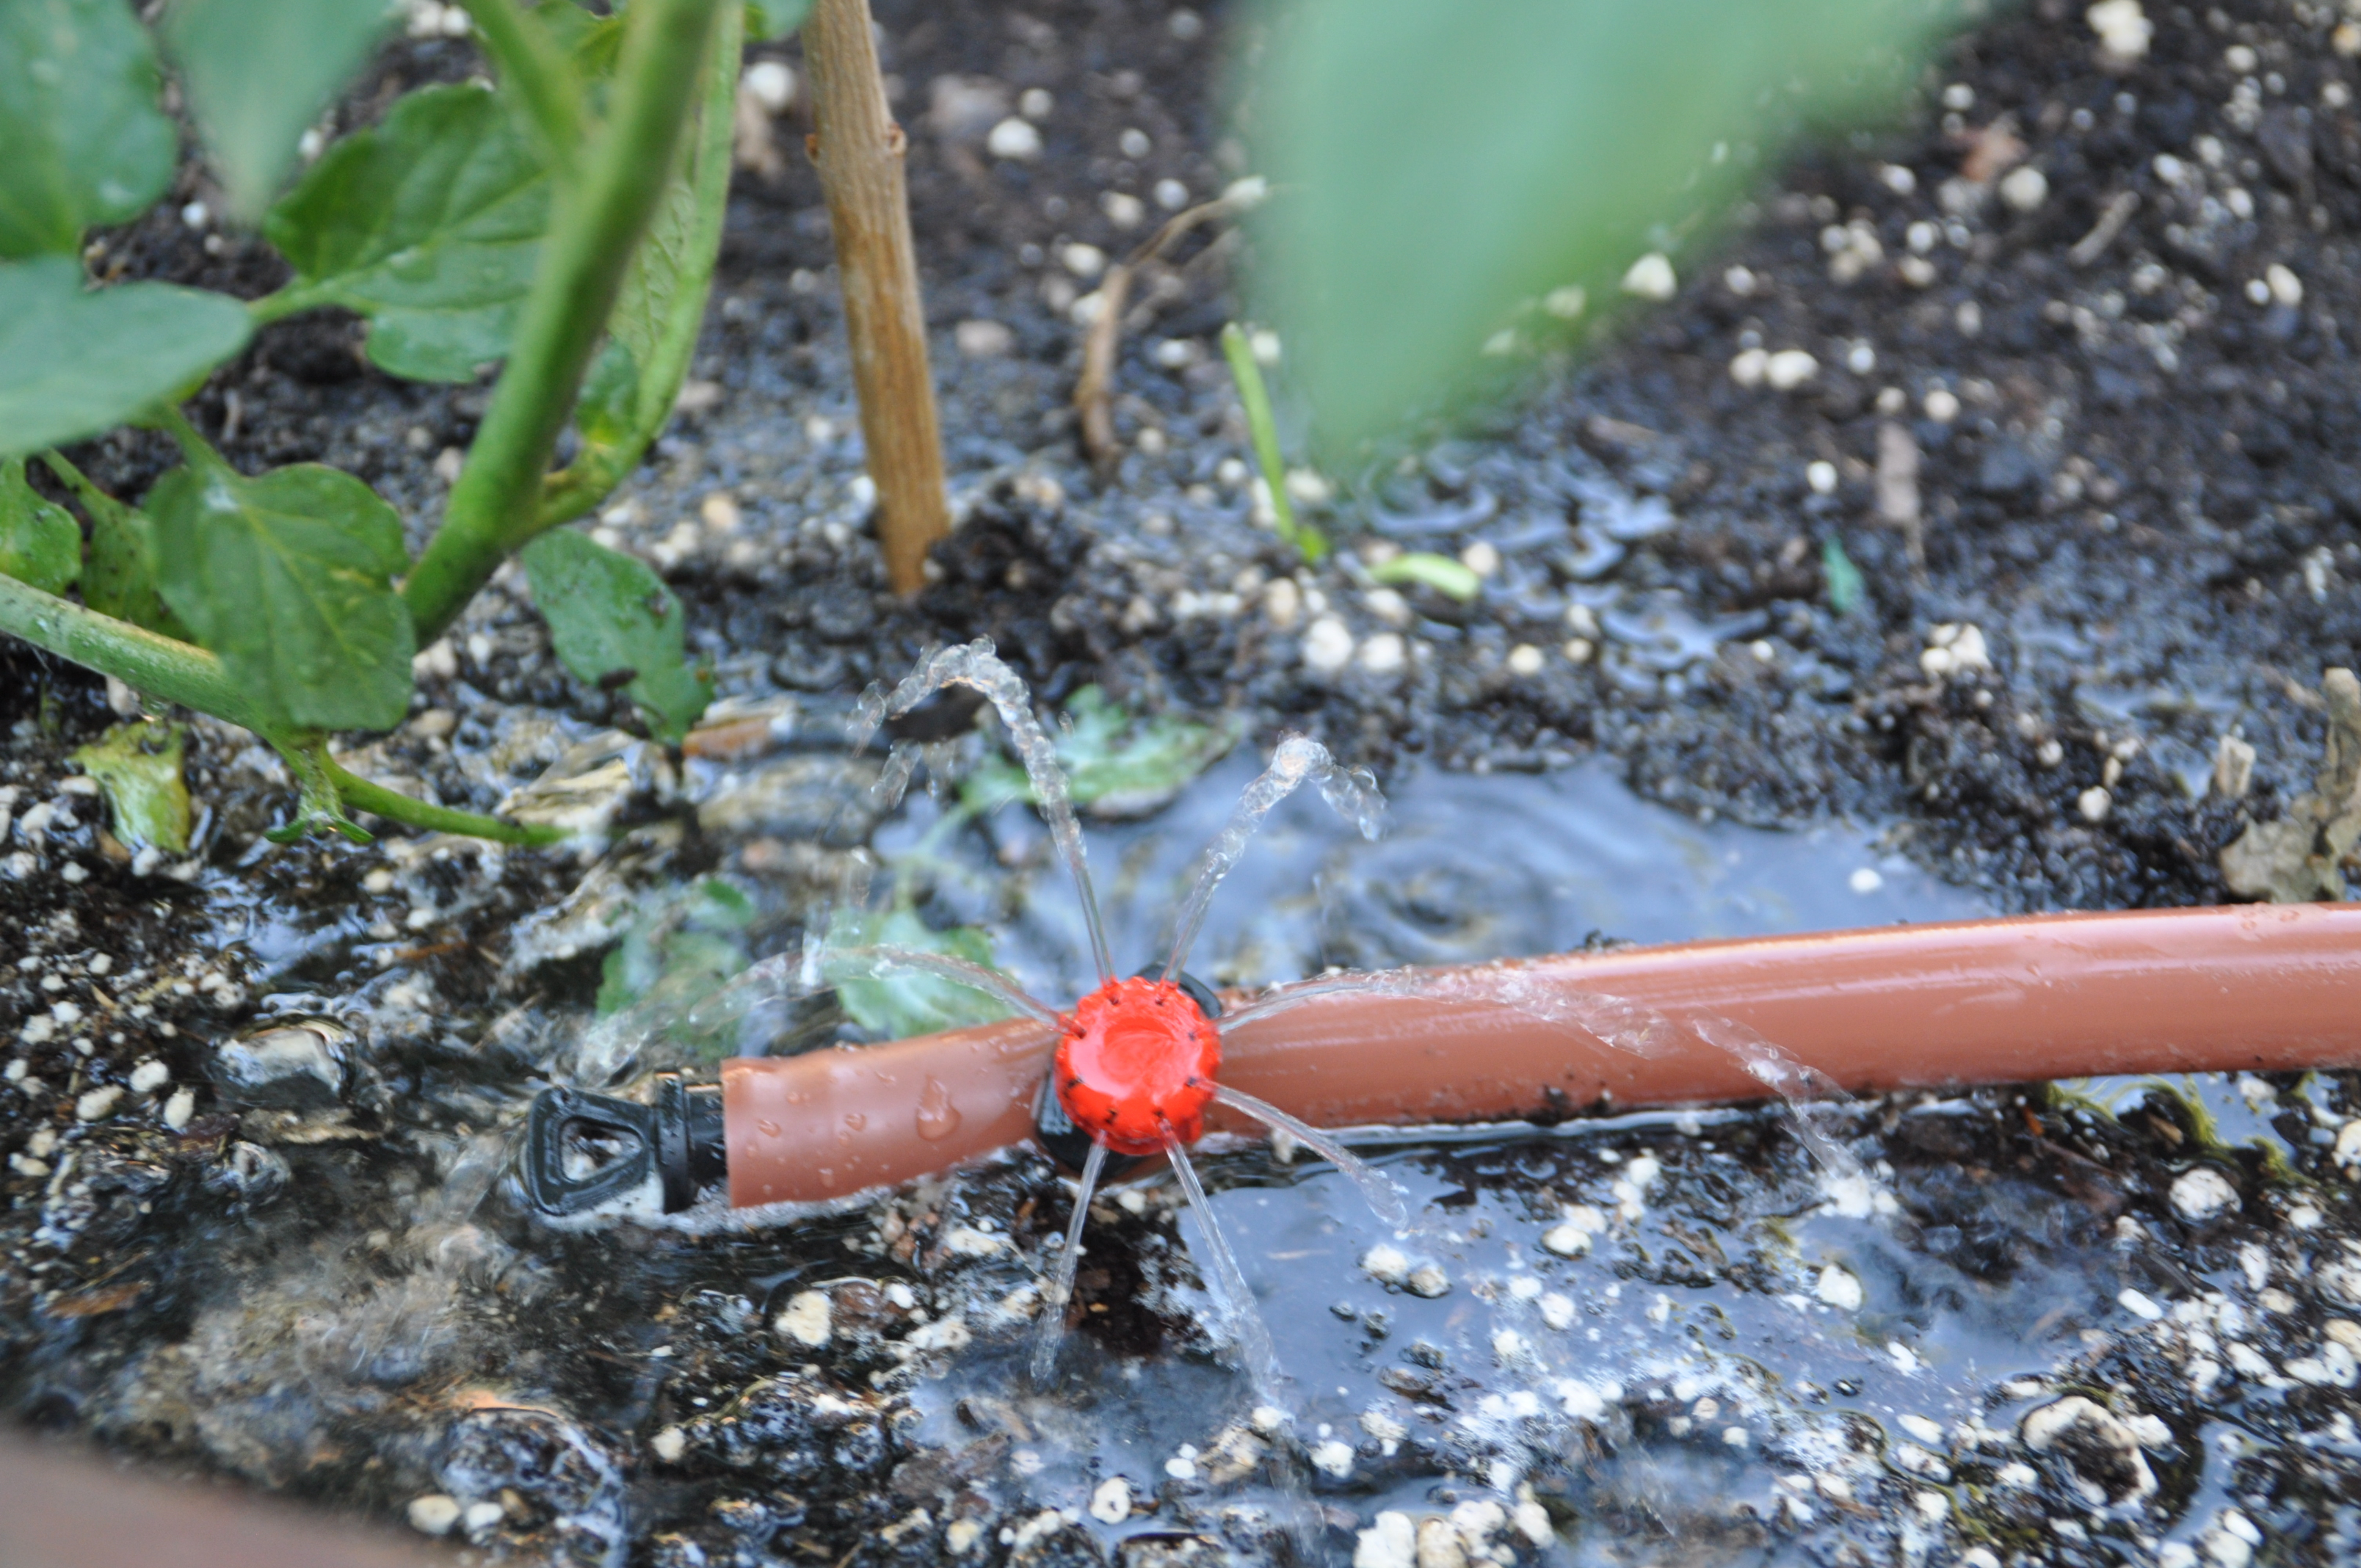
\includegraphics[width=\textwidth]{img/salidas_agua}
    \caption{Puntos de salida de agua tipo araña para realizar el riego.}
    \label{figura:salidas_agua}
  \end{minipage}
\end{figure}
    
Se ha utilizado una caja de registro hermética para proteger toda la electrónica como se muestra en las figuras~\ref{figura:caja_registro_abierta} y~\ref{figura:caja_registro_cerrada} . Esta caja está situada dentro del invernadero y contiene el Arduino y la Raspberry Pi, donde se ejecuta el software que se detallará en la sección~\ref{sec:Arquitectura e implementación software} y la protoboard y el módulo de relés detallados en la sección~\ref{sec:hardware}. De la caja salen los cables que están conectados a los sensores, colocados en su ubicación final.
\begin{figure}[H]
  \centering
  \begin{minipage}[b]{0.4\textwidth}
    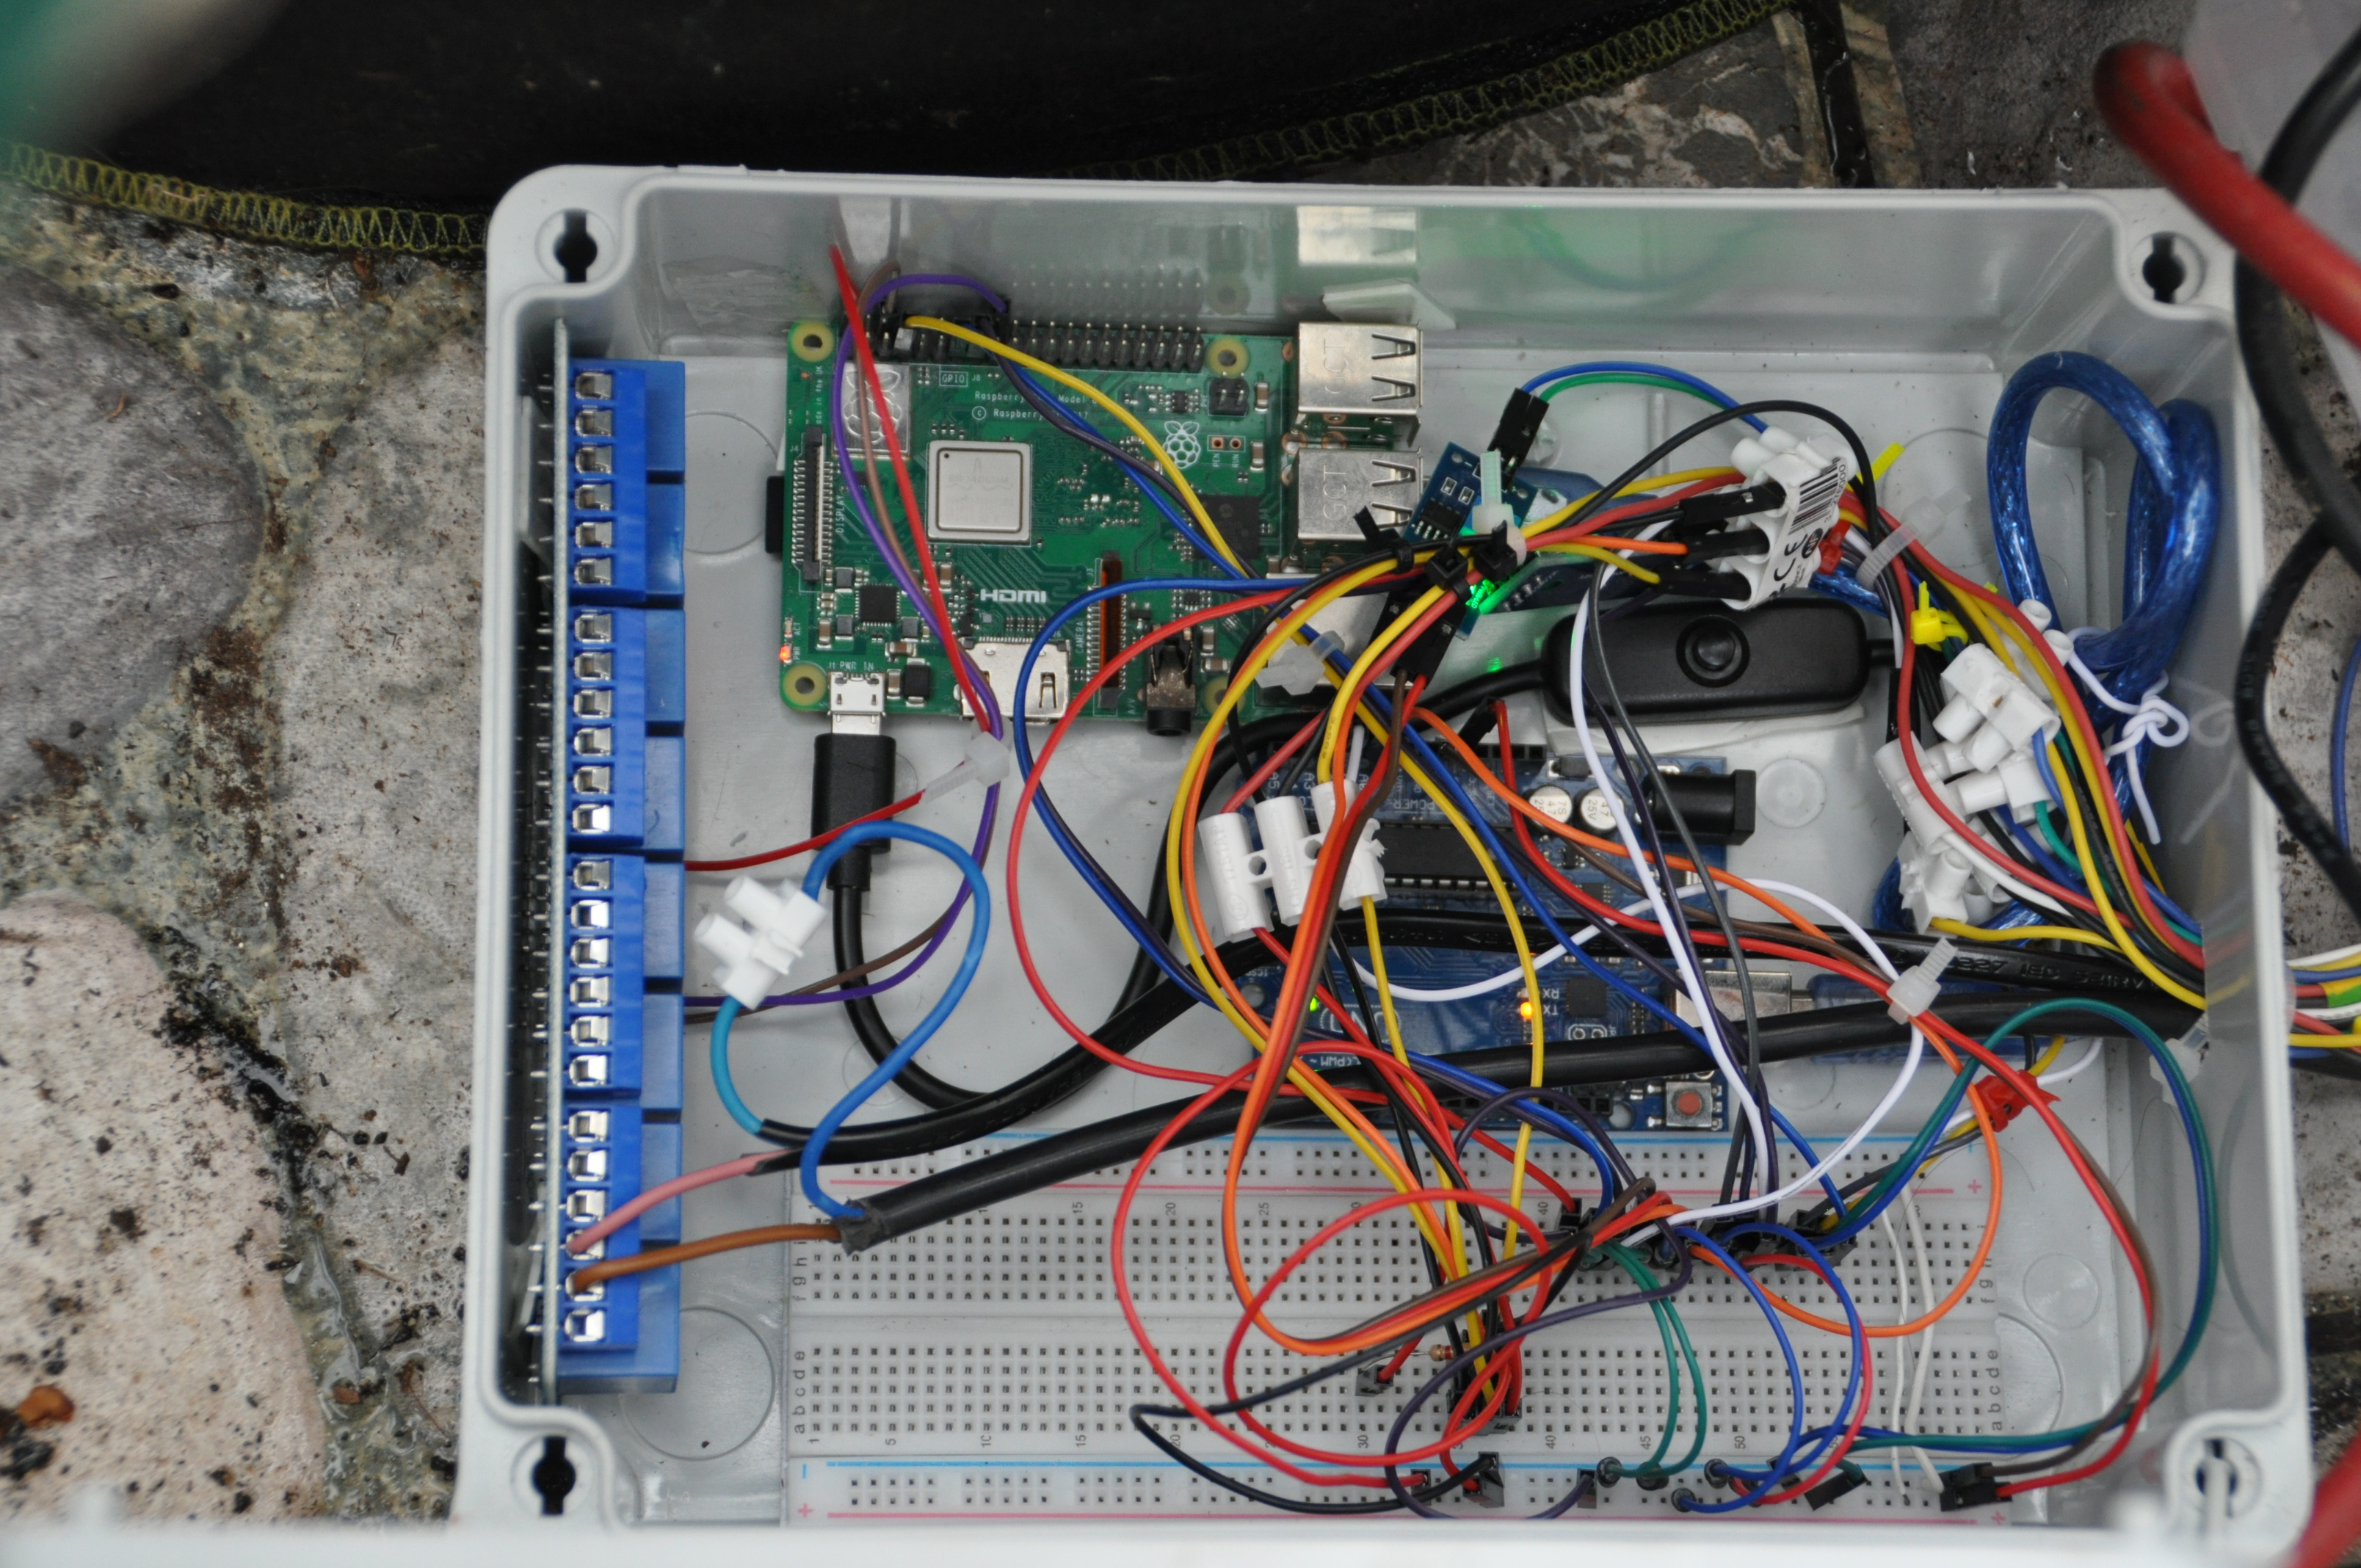
\includegraphics[width=\textwidth]{img/caja_registro_abierta}
    \caption{Caja de registro abierta.}
    \label{figura:caja_registro_abierta}
  \end{minipage}
  \hfill
  \begin{minipage}[b]{0.4\textwidth}
    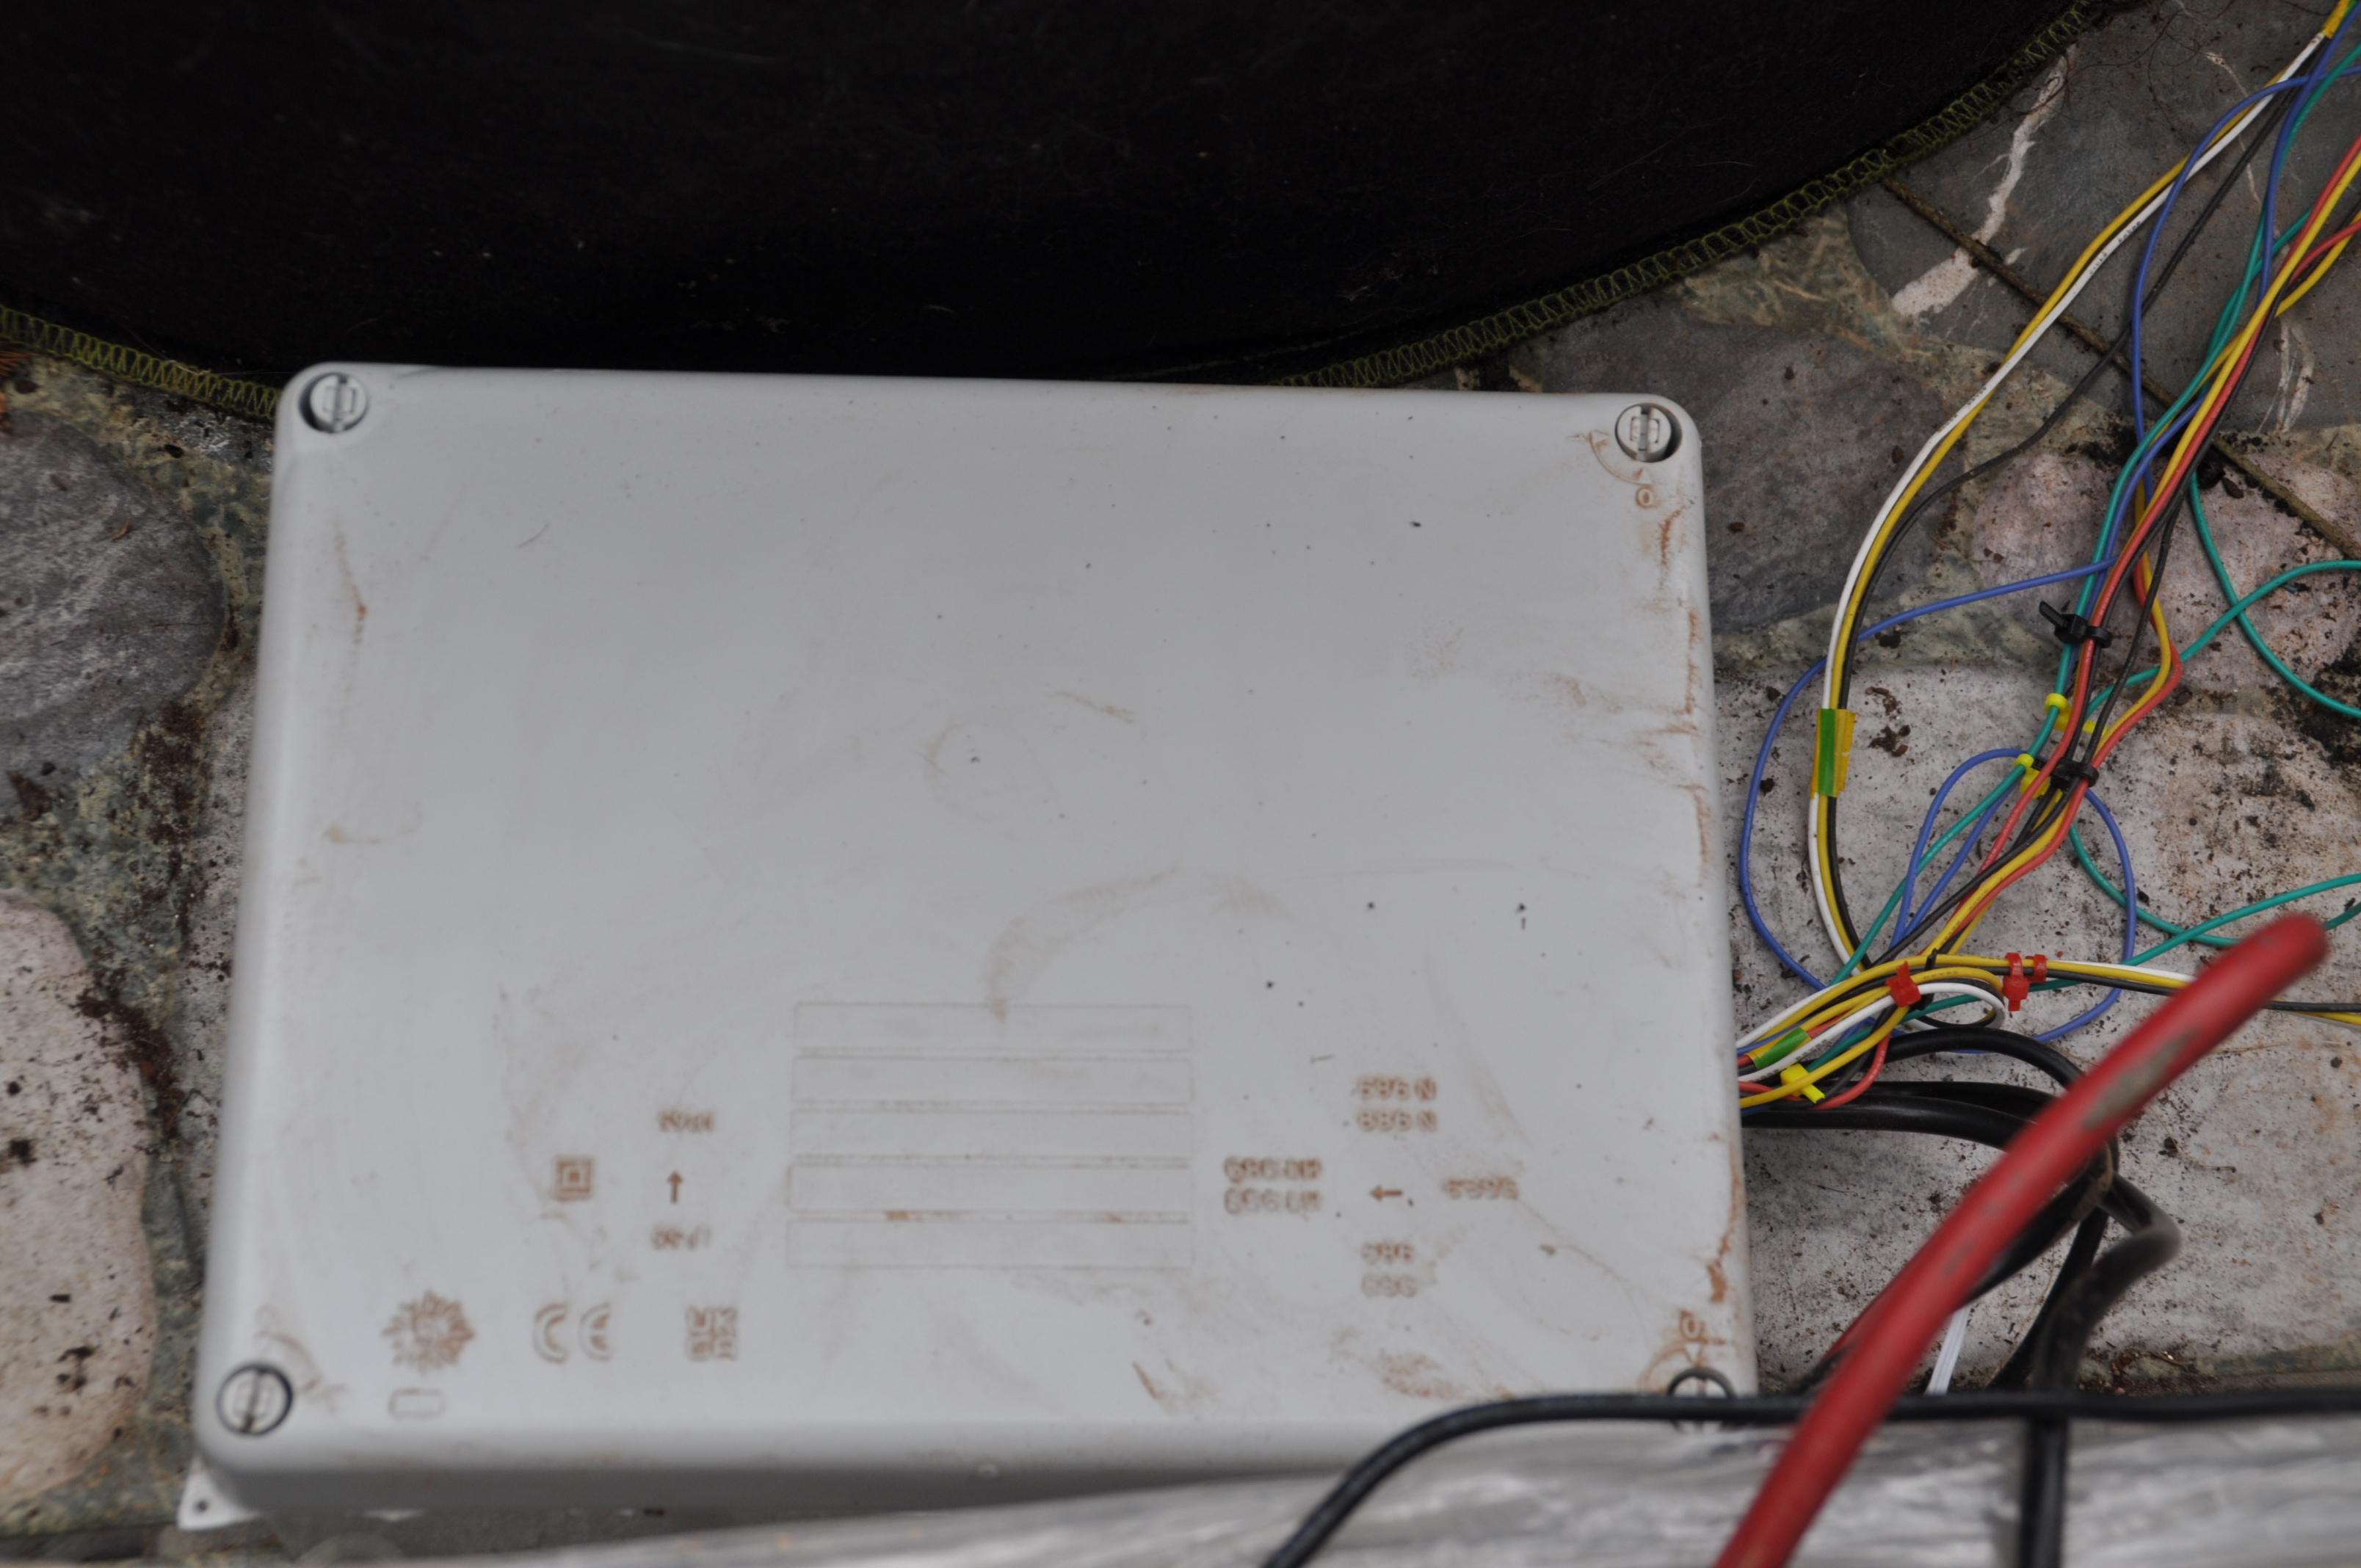
\includegraphics[width=\textwidth]{img/caja_registro_cerrada}
    \caption{Caja de registro cerrada.}
    \label{figura:caja_registro_cerrada}
  \end{minipage}
\end{figure}

Los sensores que miden humedad y temperatura ambiente se han colocado por parejas de manera que uno de ellos se encuentra fuera del invernadero y su pareja en el interior. Esto permite realizar comparativas entre la temperatura y la humedad externa y la interna. Los sensores de humedad y temperatura de la tierra se han colocado cercanos entre sí para poder realizar las pruebas del sistema, como por ejemplo poder monitorizar una sola zona de la tierra y comprobar la diferencia entre sus medidas o comprobar que estos funcionan correctamente.    

\section{Arquitectura e implementación hardware}
\label{sec:Arquitectura e implementación hardware}
El montaje de la electrónica que se presenta en este apartado incluye, como se especifica en el apartado~\ref{sec:hardware}, un microcomputador Raspberry Pi Model 3B+, conectado por su puerto USB a una placa Arduino y varios sensores y actuadores conectados a ambos dispositivos.

La Raspberry Pi está conectada al Arduino usando los puertos USB de ambos dispositivos.

La placa Arduino cuenta con pines analógicos, que no se encuentran en la Raspberry Pi. Estos pines permiten utilizar sensores analógicos que abaratan significativamente los costes del proyecto. Un ejemplo de este tipo de sensor son los higrómetros que han sido utilizados en este TFG. Una solución alternativa a este problema sería utilizar un conversor analógico-digital, aunque el coste total ascendería. La elección de la primera opción se debe principalmente a dos motivos, primero, como se ha mencionado anteriormente, es más barato un Arduino que un conversor de este tipo y segundo, nos proporciona una mayor cantidad de pines analógicos, digitales y de salida de voltaje para poder extender el modelo implementado o añadir nuevos sensores en proyectos futuros.

A continuación se detalla el montaje de cada uno de los sensores explicados en la sección~\ref{subsec:sensores}. Cada sensor cuenta con tres entradas diferentes: la entrada de datos, la entrada de voltaje (VCC) y la de tierra (GND). La entrada de datos ha sido conectada a las placas como se muestra a continuación, las entradas de voltaje y tierra a una protoboard. 

\begin{itemize}
	\item El primer módulo con sensor DHT22 al GPIO 17 de la Raspberry.
	\item El segundo módulo con sensor DHT22 al GPIO 27 de la Raspberry.
		\item La primera sonda DS18B20 al GPIO 04 de la Raspberry.
	\item La segunda sonda DS18B20 al GPIO 04 de la Raspberry.
	\item El primer módulo YL-69 al pin A0 del Arduino.
	\item El segundo módulo YL-69 al pin A1 del Arduino.
\end{itemize}

Con respecto a los sensores DS18B20 cabe destacar que ofrecen la posibilidad de realizar lecturas en serie de varios dispositivos. Este tipo de sensores utiliza el protocolo \textit{1-Wire} y permite conectar más de un sensor en el mismo bus para realizar la comunicación. Esto permite utilizar menos entradas, lo que facilita la inclusión de nuevos sensores en el futuro al disponer de más pines para conectarlos.

Tal y como se ha comentado anteriormente, además de la entrada de datos es fundamental conectar cada sensor y actuador a una fuente de alimentación y a tierra. Para facilitar la gestión del cableado, se ha utilizado una protoboard. La protoboard ha sido alimentada con el pin de 5V y GND del Arduino. Todas las conexiones electrónicas se han realizado usando cables dupont, macho-hembra, macho-macho o hembra-hembra según procediese.

\begin{figure}[H]
	\centering
    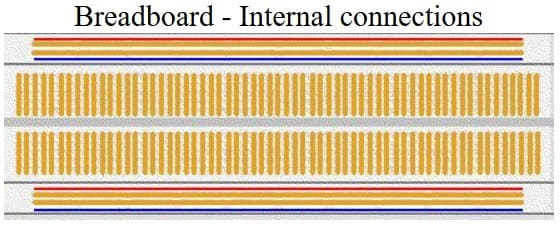
\includegraphics[width=8cm, keepaspectratio]{img/protoboard-conexiones-internas}
    \caption{Conexiones internas Protoboard.}
    \label{figura:conexiones_protoborad}
\end{figure}

El conexionado de todos los sensores es equivalente. En la figura~\ref{figura:conexion_sensor} se muestra un esquema del conexionado para un sensor.
\begin{figure}[H]
	\centering
    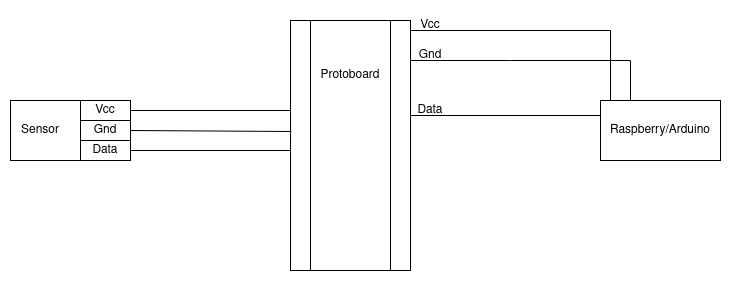
\includegraphics[width=8cm, keepaspectratio]{img/conexion_sensor}
    \caption{Esquema de conexionado de un sensor.}
    \label{figura:conexion_sensor}
\end{figure}


Como se indica en el apartado~\ref{subsec:actuadores}, para controlar los actuadores desde el software desarrollado en este TFG se ha añadido un módulo de relés, conectado a la Raspberry Pi. La bomba de agua está conectada a la corriente eléctrica doméstica (240 V), por lo que no se puede alimentar directamente con el voltaje proporcionado por la Raspberry o el Arduino. Para poder apagar o encender los actuadores, se ha colocado el relé en serie a modo de interruptor entre dos de los bornes del actuador, que estará conectado a la corriente eléctrica.
El diagrama de la figura~\ref{figura:circuito_reles} muestra cómo se ha diseñado dicho circuito.

\begin{figure}[H]
	\centering
    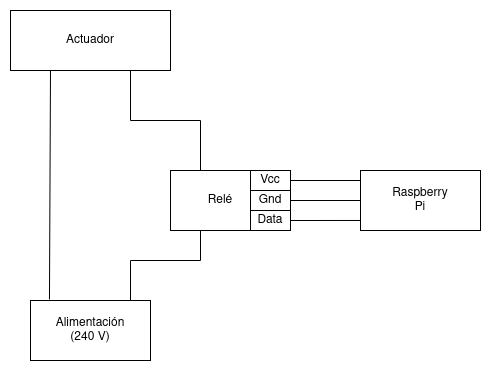
\includegraphics[width=8cm, keepaspectratio]{img/circuito_reles}
    \caption{Esquema de conexionado para un actuador.}
    \label{figura:circuito_reles}
\end{figure}

A su vez, cada uno de los actuadores está asociado a un pin GPIO de la Raspberry, en concreto, la bomba CESFONJER está asociada al GPIO 24. Físicamente, esta conexión se realiza mediante tres cables dupont que conectan el módulo de relés con la Raspberry Pi, para las entradas de VCC (voltaje de corriente continua), tierra y datos.

%El motivo de utilizar un módulo de relés en lugar de utilizar uno solo es, de nuevo, abrir la posibilidad de poder añadir nuevos actuadores de una manera sencilla.

	
\section{Arquitectura e implementación software}
\label{sec:Arquitectura e implementación software}
En esta sección se presenta la arquitectura que se ha seguido para realizar el diseño y la implementación del software en este TFG.

\subsection{Arquitectura general}
\label{subsec:arquitectura general}
El código desarrollado en este TFG está disponible en Github \footnote{\url{https://github.com/rinvictor/TFG}}. El repositorio se divide en \textit{code/}, donde se puede encontrar todo el código desarrollado, y en \textit{doc/}, que contiene la memoria.
En \textit{code/} podemos encontrar otras cinco subcarpetas:
\begin{itemize}
\item \textit{apps}, código para el desarrollo de las aplicaciones que se han realizado.
\item \textit{backup}, código para realizar un backup de la base de datos.
\item \textit{controllers}, código relativo a los actuadores.
\item \textit{datacollecting}, código relativo a la recolección de datos y los sensores.
\item \textit{modules}, credenciales de acceso a la base de datos.
\item \textit{test}, test para comprobar el correcto funcionamiento de los sensores.
\end{itemize}

En la figura~\ref{figura:esquema_general_software} se muestra la arquitectura del software implementado en este TFG. Se han realizado dos aplicaciones relativas a la visualización de datos y monitorización del sistema, una aplicación web para la visualización de datos con Dash, que se ha desplegado en Heroku\footnote{\url{https://greenhouse-tfg.herokuapp.com}}, y un bot de Telegram\footnote{\url{t.me/greenhouseTFGBot}}, que está desplegado en la propia Raspberry, y que permite además recibir notificaciones sobre el estado del invernadero, las medidas tomadas y los actuadores.
Existe también, una aplicación para controlar el riego en el invernadero mediante los actuadores del sistema.

\begin{figure}[H]
	\centering
    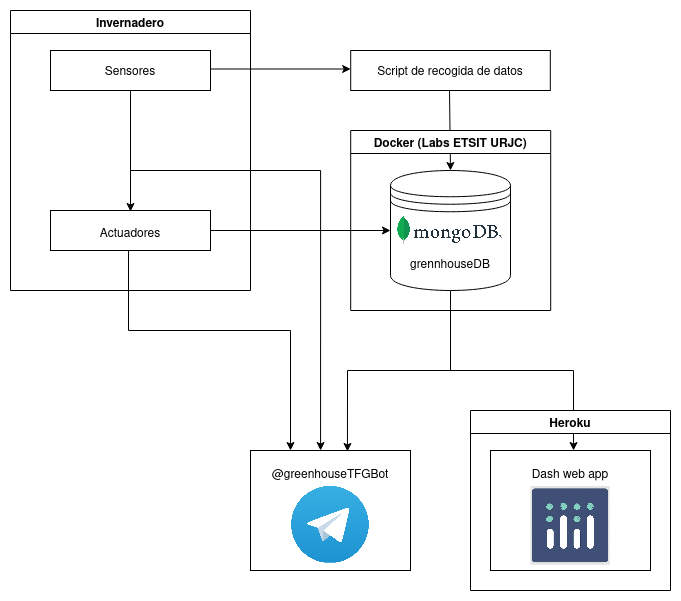
\includegraphics[width=8cm, keepaspectratio]{img/esquema_general_software}
    \caption{Esquema de la implementación software del sistema.}
    \label{figura:esquema_general_software}
\end{figure}

La figura~\ref{figura:estructura_bd} muestra la base de datos que se ha utilizado. La base de datos se ha desplegado en los laboratorios docentes de la ETSIT de la URJC en un contenedor Docker, en concreto en la máquina \textit{l2018-pc05.aulas.etsit.urjc.es}. Esta base de datos consta de dos colecciones, \textit{sensors\_data} y \textit{controllers\_data}. En \textit{sensors\_data} se almacenan los datos relacionados con la información obtenida por los sensores mientras que en \textit{controllers\_data} se almacenan la información relacionada con las acciones que toman los actuadores.

En la figura ~\ref{figura:sensors data collection} se muestra la arquitectura que se ha elegido para guardar la información de los sensores. Por cada lectura se almacenan seis valores: el ID del documento, el ID del sensor, el tipo de dato que se almacena, es decir, la magnitud medida, el valor leído, la fecha de lectura y la localización del sensor. Esta información queda almacenada en la colección \textit{sensors\_data}.

En la figura~\ref{figura:controllers data collection} se puede observar la arquitectura para la información sobre las acciones tomadas por los actuadores. En cada documento se almacena el ID del documento, el ID del actuador, la fecha de la acción realizada y el tipo de acción, por ejemplo, riego. Estos valores quedan almacenados en la colección \textit{controllers\_data}.

\begin{figure}[H]
	\centering
    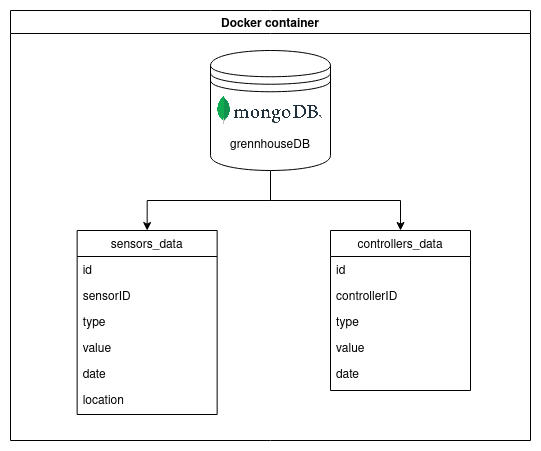
\includegraphics[width=8cm, keepaspectratio]{img/estructura_db}
    \caption{Esquema general de la estructura de la base de datos.}
    \label{figura:estructura_bd}
\end{figure}
\begin{figure}[H]
	\centering
    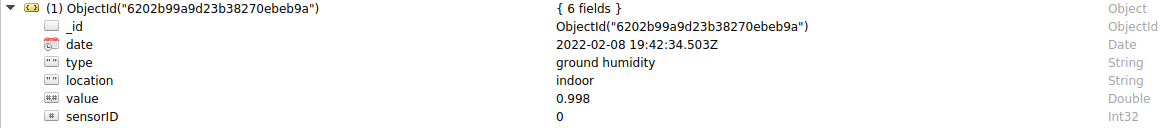
\includegraphics[width=15cm, keepaspectratio]{img/sensors_data_collection}
    \caption{Estructura de la colección \textit{sensors\_data}, perteneciente a la base de datos \textit{greenhouseDB}.}
    \label{figura:sensors data collection}
\end{figure}
\begin{figure}[H]
	\centering
    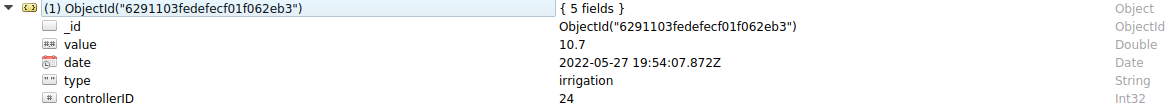
\includegraphics[width=15cm, keepaspectratio]{img/controllers_data_collection}
    \caption{Estructura de la colección \textit{controllers\_data}, perteneciente a la base de datos \textit{greenhouseDB}.}
    \label{figura:controllers data collection}
\end{figure}

Se realiza una copia de seguridad de cada una de las colecciones de la base de datos una vez al día, dejándola en dos archivos \textit{.csv}. De esta manera el sistema puede sobreponerse al borrado no intencionado de la información como por ejemplo, si el contenedor Docker en el que está desplegada la base de datos es borrado.
El código para realizar este backup se localiza en \textit{code/backup}. La lógica del proceso se encuentra en \textit{backup.py} mientras que el proceso que lanza la lógica se encuentra en \textit{execute\_backup.sh}. 
Al ejecutar el proceso anterior se almacenan los mensajes en \textit{code/backup/logs/success.log} si todo funciona correctamente, en \textit{code/backup/logs/error.log} si falla y en \textit{code/backup/logs/cronerror.log} si es cron el que encuentra problemas para ejecutar el proceso.

El software para la de recogida de datos, control de actuadores y el bot de Telegram se ha desplegado en la Raspberry Pi, mientras que la aplicación web se ha desplegado en la nube y la base de datos está alojada en los laboratorios docentes de la URJC. De esta forma, si hubiera una rotura o una caída de la red en la Raspberry podría detectarse rápidamente a través de la aplicación web, y los datos almacenados hasta el momento no se perderían y podrían seguir siendo consultados. Por otro lado, la caída de la aplicación web no afectaría al funcionamiento de la Raspberry Pi y todos los procesos ejecutados en ella continuarían. Por último, si la base de datos dejase de funcionar se podría detectar rápidamente a través de los logs de la Raspberry y mediante el bot de Telegram.
 
Los scripts de recogida de datos, creación del backup de la base de datos, comprobación de la calidad de los datos y la toma de acciones se lanzan en segundo plano utilizando Cron. A continuación se muestra el fichero de configuración para lanzar dichos scripts.

\begin{lstlisting}
1 */2 * * * /home/pi/TFG/code/datacollecting/execute.sh > /home/pi/TFG/code/datacollecting/logs/cronerror.log 2>&1
10 */2 * * * /home/pi/TFG/code/apps/telegram/execute_monitoring.sh > /home/pi/TFG/code/apps/telegram/logs/cronerror.log 2>&1
1 */24 * * * /home/pi/TFG/code/backup/execute_backup.sh > /home/pi/TFG/code/backup/logs/cronerror.log 2>&1
30 */24 * * * /home/pi/TFG/code/apps/actions/execute_actions.sh > /home/pi/TFG/code/apps/actions/logs/cronerror.log 2>&1
\end{lstlisting}

Se pueden observar los diferentes \textit{.sh} que se han desarrollado para ejecutar las aplicaciones y como, en caso de fallo, se escribe el fichero \textit{cronerror.log}.
En \textit{execute.sh} se lanza el software para la recogida de datos, \textit{execute\_monitoring.sh} es el encargado de lanzar el software para comprobar la calidad de los datos y el correcto funcionamiento de los sensores, \textit{execute\_backup.sh} lanza el backup de la base de datos y \textit{execute\_actions.sh} lanza el software para controlar los actuadores y realizar acciones. La funcionalidad de estos scripts es comentada en las siguientes secciones.

\subsection{Recogida de datos}
\label{subsec:recogida de datos}
La recogida de datos, como se ha mencionado anteriormente, se realiza en la propia Raspberry. Para implementar esta funcionalidad se han creado varios ficheros y el código está disponible en \textit{code/datacollecting}. En primer lugar, se ha creado el fichero de configuración \textit{config.py} en el cual se implementa la clase Sensor, que facilita la gestión de la localización de los sensores y de los pines a los que están conectados.

\begin{lstlisting}[language=Python]
class Sensor:
    def __init__(self, pin, location):
        self.pin = pin
        self.location = location
\end{lstlisting}

Todos los sensores en este TFG se representan en el código con instancias de la clase \textit{Sensor}. El pin al que está conectado se utiliza a modo de identificador único ya que varios sensores no pueden estar conectados al mismo pin. El caso de los sensores DS18B20 es diferente, ya que como se explica en el apartado~\ref{sec:Arquitectura e implementación hardware} estos sensores si pueden estar conectados a un mismo pin, por lo que se utiliza su identificador hardware como identificador único. La localización indica si el sensor se encuentra dentro o fuera del invernadero.

Los scripts para la recogida de datos se han implementado en los ficheros \textit{sensors.py} y \textit{db\_conn.py}. En \textit{sensors.py} se definen las diferentes funciones que permiten leer la información de los sensores, habiendo implementado una función para cada tipo de sensor. Para este propósito se han utilizado distintas librerías que permiten controlar los sensores: \textit{pyfirmata2} para los sensores YL-69, \textit{Adafruit\_DHT} para los sensores DHT22 y \textit{w1thermsensor} para los DS18B20.
Existen las funciones \textit{get} y las funciones \textit{read}. Las primeras sirven para manejar los datos recogidos por las funciones \textit{read} de tal manera que las funciones \textit{read} se encargan de leer los datos mediante los sensores y las funciones \textit{get} de obtenerlos para manejarlos desde distintos puntos en el software.

En el fichero \textit{db\_conn.py} se implementa la funcionalidad relativa a la inserción de los datos en la base de datos \textit{greenhouseDB} de MongoDB, en concreto en la colección \textit{sensors\_data}. Antes de insertar la información en la base de datos, se valida para detectar inconsistencias. En el caso de caso de que la lectura sea nula (en Python \textit{None}) o que sea un valor fuera de un rango establecido (por ejemplo, 120 ºC de temperatura es un error) se almacena un -1. Puede interesar conocer, por ejemplo, la tasa de fallo de un sensor. Es por este motivo por el que no se reintenta la lectura de los datos en caso de error. Un fallo en una lectura queda escrito en los ficheros de \textit{log} y, además, se le comunica al usuario vía Telegram tal y como se detallará en el próximo capítulo de esta memoria.
A continuación se muestra un pequeño fragmento a través del cual se inserta el valor de la temperatura ambiente medida por los sensores DHT22 en la base de datos. Como se puede observar, se almacena el tipo de dato, el valor obtenido, el ID del sensor, la localización y la fecha de captura del dato.


\begin{lstlisting}[language=Python]
        now = datetime.now()

        item = {"type": "ambient temperature", "value": ambient_temperature, "sensorID": d.pin, "location": d.location,
                "date": now}
        collection.insert_one(item)
\end{lstlisting}

Se ha desarrollado un script de Bash donde se lanzan los scripts de Python encargados de la recolección de datos, además se realizan las exportaciones de módulos de Python pertinentes y se almacena el resultado del proceso en los ficheros de log. El script de Bash sí realiza reintentos, de tal manera que si es la aplicación la que falla relanza su ejecución. En caso de fallo se almacena el resultado con la etiqueta \textit{Exec Error}. En caso de fallar este segundo reintento la etiqueta pasa a ser \textit{Fatal Error}. Si el segundo intento tiene éxito, se escribe en el fichero de log indicando que ha sido tras un reintento. Todos los ficheros de log se escriben con la fecha y el resultado de la ejecución.
A continuación se muestra un ejemplo de la información que se almacena en los \textit{logs}.

\begin{lstlisting}[language=Bash]
vie may 27 20:01:27 CEST 2022 success {'type': 'ground humidity', 'value': 0.2278, 'sensorID': 0, 'location': 'indoor', 'date': datetime.datetime(2022, 5, 27, 20, 1, 8, 24826), '_id': ObjectId('629111e4b2c6d1b9a5e7f23f')} 0.2209 {'type': 'ground humidity', 'value': 0.2209, 'sensorID': 1, 'location': 'indoor', 'date': datetime.datetime(2022, 5, 27, 20, 1, 13, 710340), '_id': ObjectId('629111e9b2c6d1b9a5e7f240')} 32.0 {'type': 'ambient humidity', 'value': 32.0, 'sensorID': 22, 'location': 'outdoor', 'date': datetime.datetime(2022, 5, 27, 20, 1, 15, 457495), '_id': ObjectId('629111ebb2c6d1b9a5e7f241')} 27.200000762939453 {'type': 'ambient humidity', 'value': 27.200000762939453, 'sensorID': 27, 'location': 'indoor', 'date': datetime.datetime(2022, 5, 27, 20, 1, 17, 203246), '_id': ObjectId('629111edb2c6d1b9a5e7f242')} 28.899999618530273 {'type': 'ambient temperature', 'value': 28.899999618530273, 'sensorID': 22, 'location': 'outdoor', 'date': datetime.datetime(2022, 5, 27, 20, 1, 21, 482673), '_id': ObjectId('629111f1b2c6d1b9a5e7f243')} 32.79999923706055 {'type': 'ambient temperature', 'value': 32.79999923706055, 'sensorID': 27, 'location': 'indoor', 'date': datetime.datetime(2022, 5, 27, 20, 1, 23, 239564), '_id': ObjectId('629111f3b2c6d1b9a5e7f244')} 33.0 {'type': 'ground temperature', 'value': 33.0, 'sensorID': '325a0f1e64ff', 'location': 'indoor', 'date': datetime.datetime(2022, 5, 27, 20, 1, 25, 179596), '_id': ObjectId('629111f5b2c6d1b9a5e7f245')} 27.625 {'type': 'ground temperature', 'value': 27.625, 'sensorID': '32360c1e64ff', 'location': 'indoor', 'date': datetime.datetime(2022, 5, 27, 20, 1, 27, 99572), '_id': ObjectId('629111f7b2c6d1b9a5e7f246')}
\end{lstlisting}

Este tipo de información es útil para poder encontrar fallos en el sistema. Además de los logs resultantes del lanzamiento de los scripts desarrollados en este TFG, también se guardan los errores propios de Cron en el fichero \textit{cronerror.log}.


\subsection{Aplicación de Dash}
\label{aplicacion de dash}
En este TFG se ha desarrollado una aplicación que permite visualizar de forma gráfica la información recogida por los sensores y las acciones tomadas por los actuadores. Esta aplicación se ha implementado usando el framework Dash, descrito en la sección~\ref{subsec:dash}.
Todo el código que usa la aplicación se encuentra dentro de \textit{code/apps/dashapp}.
Para el desarrollo de la aplicación se han utilizado los componentes html y CSS integrados en Dash además de una plantilla libre de Bootstrap para componer el estilo de la página \footnote{\url{https://bootswatch.com/sandstone}}.

La aplicación tiene varios componentes, \textit{app.py}, programa principal, \textit{dash\_utils.py},  donde se han implementado funciones de filtrado y \textit{create\_figures.py}, donde se implementa la generación de las visualizaciones utilizando la librería \textit{Plotly}.

Una vez se lanza la aplicación y se accede a ella a través del navegador, se encuentran las siguientes funcionalidades, tal y como se muestra en la figura~\ref{figura:web}

\begin{itemize}
\item \textit{HOME}, página principal.
\item \textit{SENSORS DATA}, un desplegable con las magnitudes medidas.
\item \textit{CONTROLLERS DATA}, un desplegable con los controladores (la aplicación de riego).
\item \textit{DOCUMENTATION}, documentación del proyecto.
\end{itemize}

\begin{figure}[H]
	\centering
    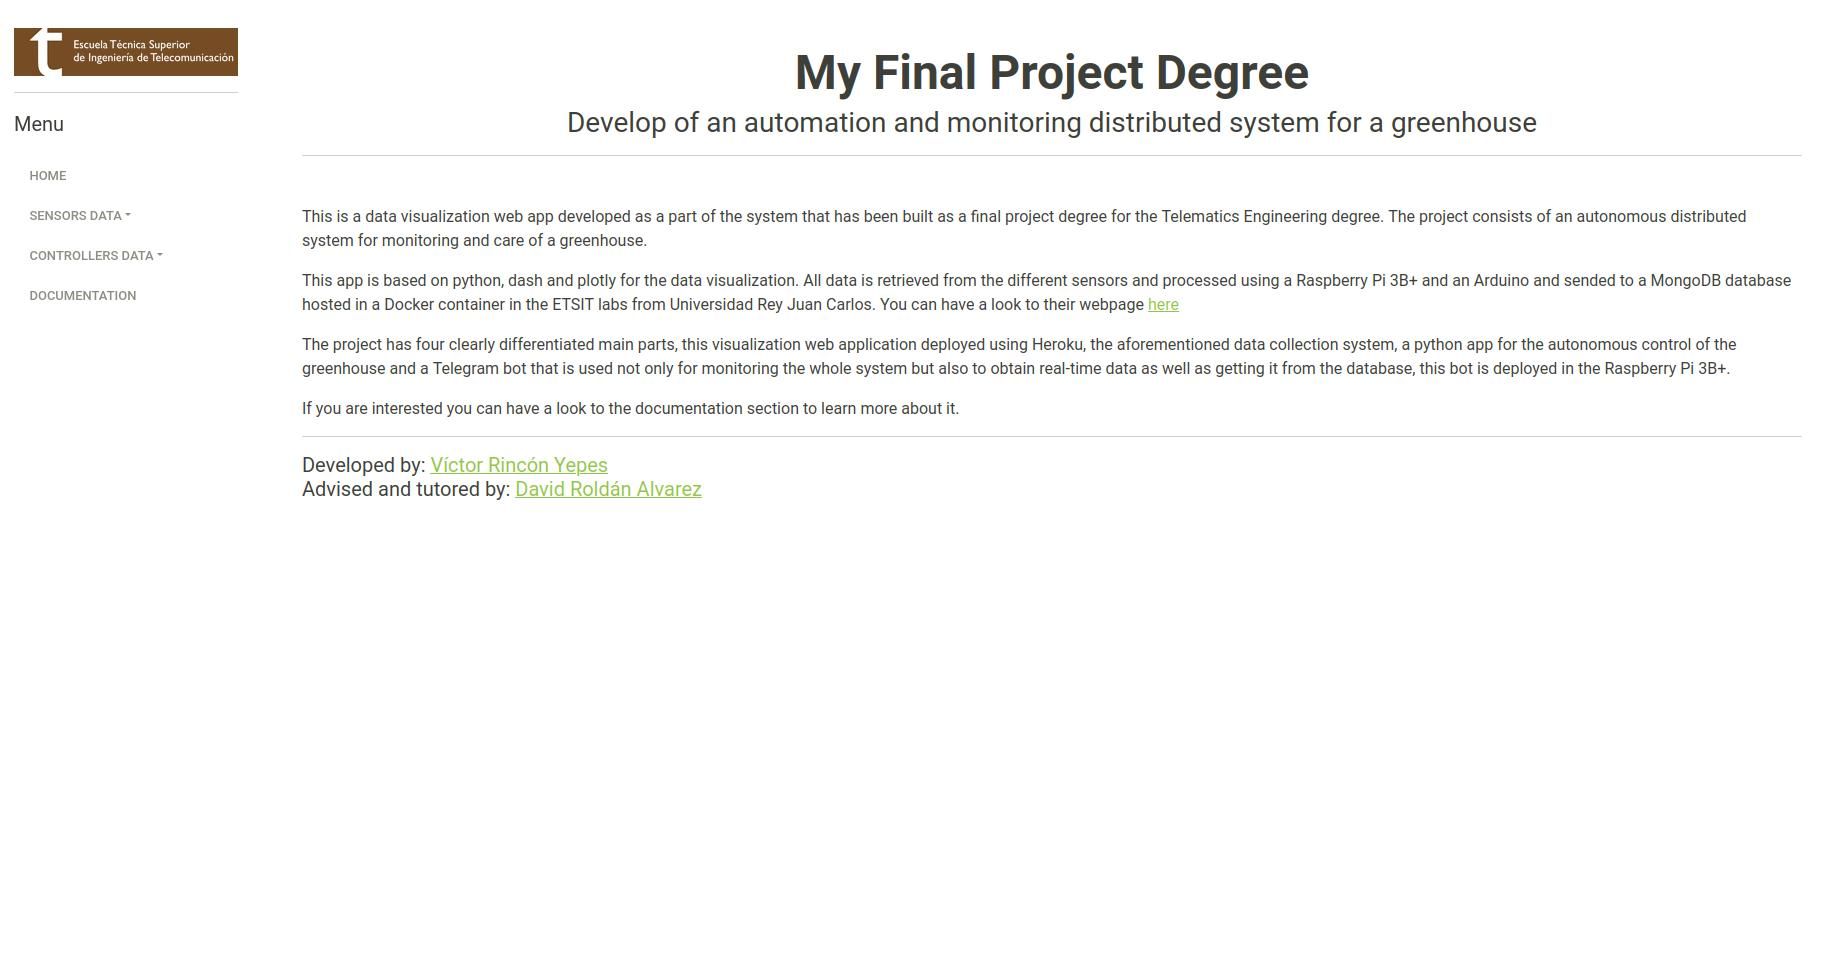
\includegraphics[width=12cm, keepaspectratio]{img/web}
    \caption{Aplicación de visualización de datos.}
    \label{figura:web}
\end{figure}

A través de cada opción del menú se accede a la gráfica que representa la información recogida por los sensores o actuadores de un mismo tipo. Por ejemplo, en el desplegable \textit{SENSORS DATA} se pueden ver las distintas magnitudes que se miden y para las que se obtienen datos del sistema, humedad ambiente, temperatura ambiente, humedad de la tierra y temperatura de la tierra. A modo de ejemplo, en la figura~\ref{figura:humedad_ambiente_grafica} se puede observar la gráfica que representa la información recogida por el sensores 22 y 27.

\begin{figure}[H]
	\centering
    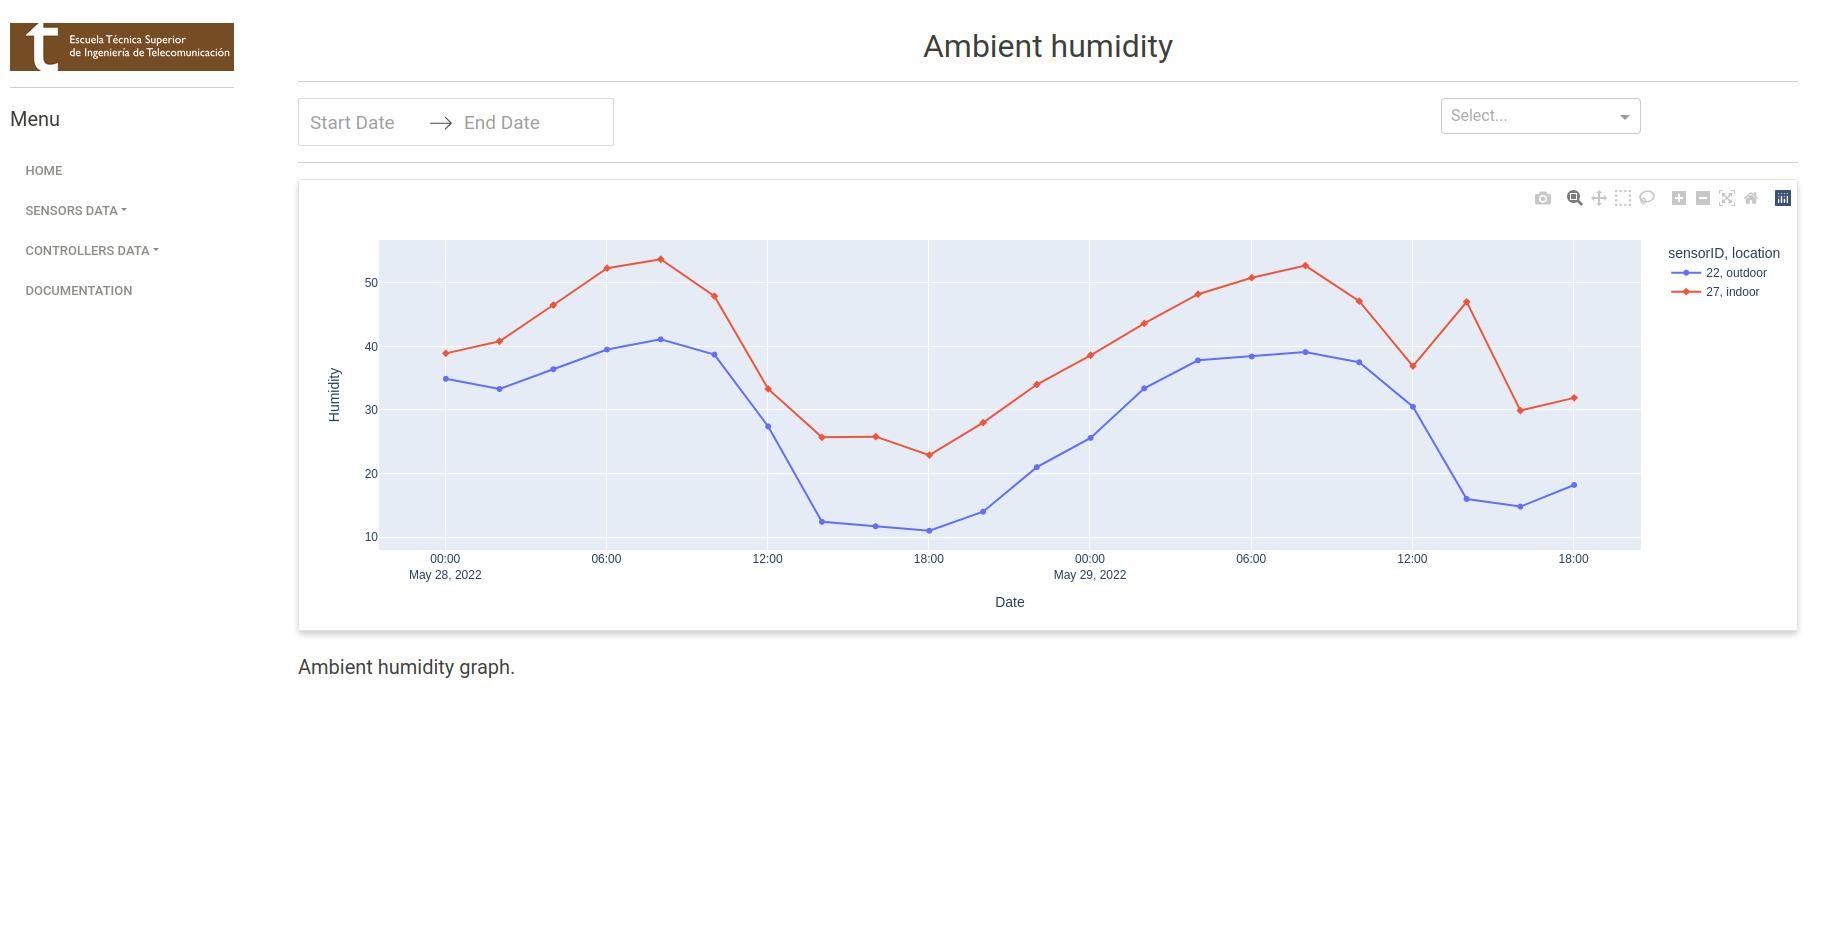
\includegraphics[width=12cm, keepaspectratio]{img/humedad_ambiente_grafica}
    \caption{Aplicación de visualización de datos.}
    \label{figura:humedad_ambiente_grafica}
\end{figure}

Entre el título de la figura y la gráfica que se observan en la figura~\ref{figura:humedad_ambiente_grafica}, se muestra que hay una serie de campos que permiten realizar filtrados en la información presentada. Por ejemplo, a través del desplegable se ha elegido el sensor 27 para mostrar únicamente la información recogida por dicho sensor, tal y como se puede ver en la figura~\ref{figura:humedad_ambiente_grafica_selectores}. Además, se han seleccionado dos fechas, de inicio y fin para presentar la información almacenada entre estas.

\begin{figure}[H]
	\centering
    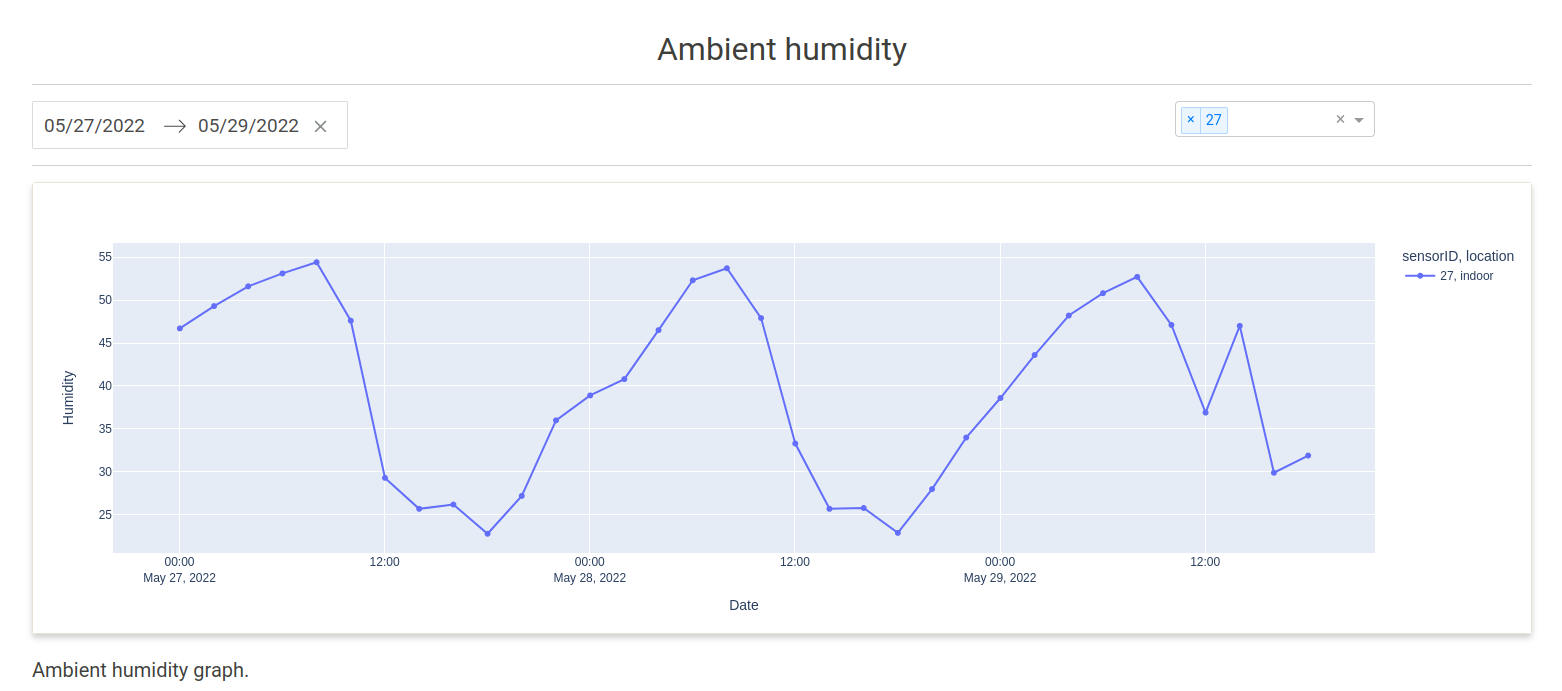
\includegraphics[width=12cm, keepaspectratio]{img/humedad_ambiente_valores}
    \caption{Cambio tras selección de fecha y sensor en la humedad ambiente.}
    \label{figura:humedad_ambiente_grafica_selectores}
\end{figure}

\begin{figure}[H]
	\centering
    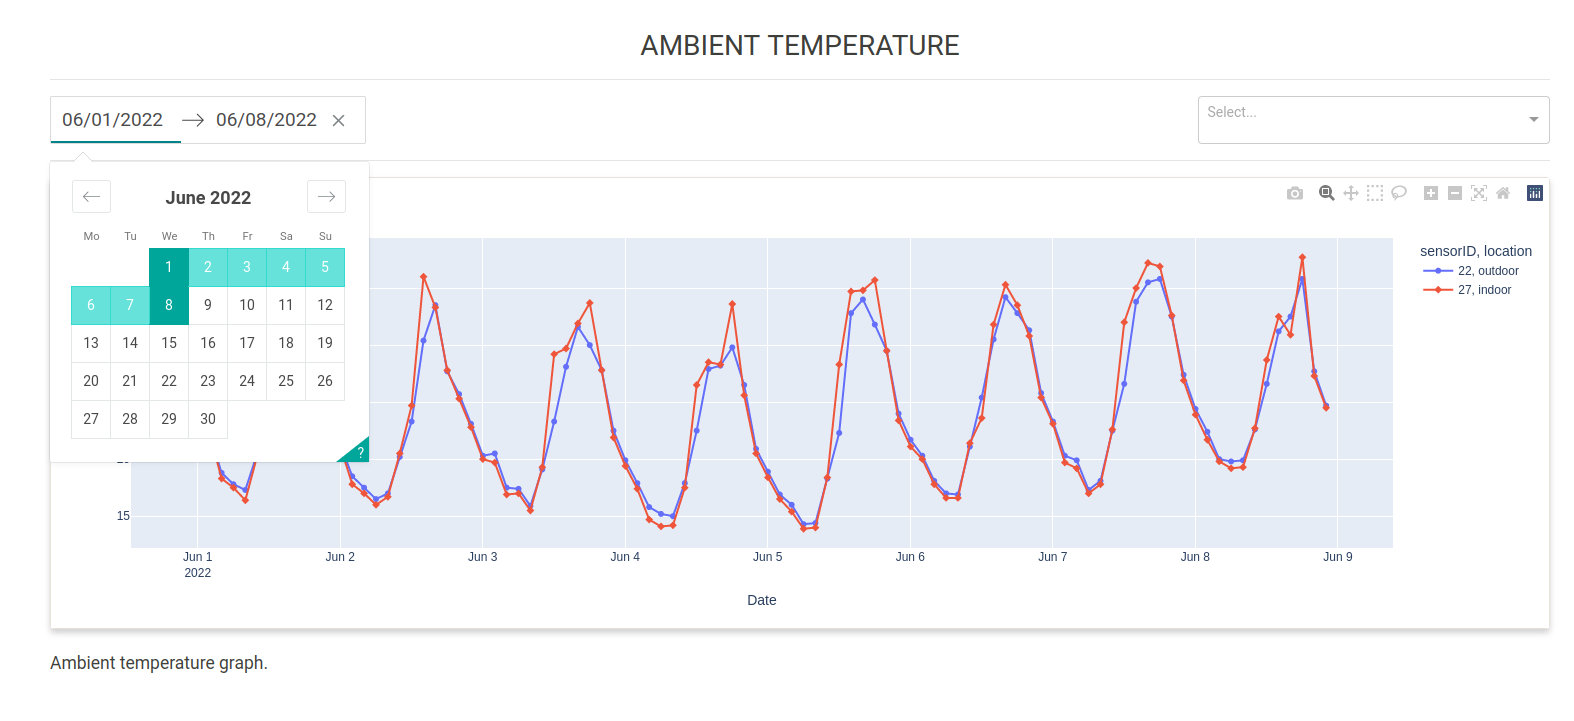
\includegraphics[width=12cm, keepaspectratio]{img/desplegable_fecha}
    \caption{Uso del selector de fechas en la aplicación web.}
    \label{figura:desplegable_fecha}
\end{figure}

Utilizando los \textit{callbacks} de Dash se pueden realizar los filtrados presentados en el párrafo anterior, lo que permite dotar de interactividad a la aplicación. Un \textit{callback} es una función que se lanza automáticamente cada vez que un componente recibe un cambio, pudiendo generar este cambio una actualización de la visualización.


El siguiente código muestra como se implementa una función \textit{callback}. En esta función, se reciben como parámetros de entrada los filtros a través de los que se establecen una fecha de inicio y de fin de los datos, así como el ID del sensor que se quiere visualizar.  En base a los filtros, se seleccionan los datos pertinentes y se genera una nueva visualización.

\begin{lstlisting}[language=Python]
@app.callback(
    Output('ambient_temperature_fig', 'figure'),
    [Input('date_picker_ambient_temperature', 'start_date'),
     Input('date_picker_ambient_temperature', 'end_date'),
     Input('dropdown_ambient_temperature', 'value')]
)
def update_output(start_date, end_date, value):
    df = getdataframe("ambient temperature")
    prev = datetime.strftime(datetime.now() - timedelta(7), '%Y-%m-%d')
    today = datetime.strftime(datetime.now(), '%Y-%m-%d')
    if not value and not start_date and not end_date:
        df = du.date_filter(df, start_date=prev, end_date=today)
    if start_date or end_date:
        df = du.date_filter(df, start_date, end_date)
    if value and len(value) > 0 and start_date and end_date:
        df = du.date_filter(df, start_date, end_date)
        df = df[df['sensorID'].isin(value)]
    if value and not start_date:
        df = du.date_filter(df, start_date=prev, end_date=today)
        df = df[df['sensorID'].isin(value)]

    fig = figures.create_temperature_fig(df)
    return fig
\end{lstlisting}

La gestión de la información dentro de la aplicación se realiza utilizando el módulo Pandas de Python. A través de este módulo resulta cómodo y sencillo interconectar la información almacenada en la base de datos MongoDB con la creación de las gráficas correspondientes.
Es muy común trabajar utilizando Pandas y MongoDB. 

A través de la aplicación Dash se hace una llamada a la base de datos, se guarda la información en un DataFrame de Pandas, que  consiste en una tabla con columnas y filas. A este DataFrame se le pueden aplicar filtros para obtener solo una parte de la información y finalmente se utiliza para crear, junto con Plotly, la gráfica que se solicite.

Esta misma funcionalidad es equivalente para mostrar los datos relativos a los actuadores, en concreto, se muestran los litros utilizados al día por la aplicación de riego, cuyo funcionamiento concreto se mostrará en la sección~\ref{subsec:riego}.

Entre las funcionalidades ofrecidas por Plotly, cabe destacar que es posible descargar las imágenes directamente y hacer zoom sobre una zona en concreto de la gráfica. 
 

\subsection{Bot de Telegram}
\label{bot de telegram}
En este TFG se ha desarrollado un bot de Telegram llamado \textit{greenhouseTFGBot}. El objetivo de este bot no es exclusivamente el de enviar mensajes al usuario sino, además, poder obtener información de los sensores, tanto en tiempo real como desde la base de datos y enviar gráficas construidas con Plotly interactuando con el usuario. En esta sección se especifican todas las funcionalidades implementadas en este bot. Ejemplos concretos y salidas de comandos pueden ser vistos en la sección~\ref{sec:aplicación de dash ejemplos}.

Este bot se ha desarrollando haciendo uso de la API de telegram y de la librería de Python Telepot. Se puede encontrar el código en \textit{code/apps/telegram} del repositorio de Github.

Para crear el bot se ha utilizado un bot propio de Telegram, llamado \textit{Botfather}, que permite crear y administrar los bots ya existentes. Al crear un bot se crea un token de identificación única que será el utilizado para poder desarrollar toda la funcionalidad y asociarla a este bot.
 
La aplicación principal se encuentra en el fichero \textit{app.py}. Como se ha comentado anteriormente, hace uso de la librería Telepot. Telepot tiene una función incluida llamada \textit{MessageLoop}. Esta función recibe dos parámetros, el objeto que hace referencia al bot, y la función \textit{handle} que manejará los mensajes que el usuario introduzca por pantalla. \textit{MessageLoop} es un bucle infinito que está en continua escucha y responde a las diferentes peticiones del usuario.

Las funcionalidades que se han incluido en este bot son:
\begin{itemize}
\item Obtener una lista con todos los comandos disponibles
\item Obtener una lista con información sobre cada uno de los sensores
\item Obtener una lista con información sobre cada uno de los actuadores
\item Obtener el estado de uno o todos los sensores en tiempo real
\item Obtener el estado de uno o todos los sensores y actuadores leyendo desde la base de datos.
\item Obtener las figuras construidas con Plotly de uno o todos los sensores y actuadores.
\item Enviar mensajes de error cuando alguna de las lecturas de cualquier sensor falle.
\item Enviar mensajes informativos sobre la ejecución de los actuadores.
\end{itemize}

Cuando el bot es lanzado con el comando \textit{/start}, el usuario recibe un mensaje con los comandos disponibles. El usuario puede volver a pedir esta información con el comando \textit{/help}.
Cuando se introduce un comando erróneo o inexistente se recibe un mensaje indicando que el comando introducido es incorrecto concatenado con la lista de comandos disponibles.

Escribiendo \textit{/sensorsinfo} se recibe una lista con información sobre cada uno de los sensores que están implementados en el sistema, indicando su id (GPIO, pin Arduino o su id de hardware). La información sobre los actuadores se recibe usando el comando \textit{/controllersinfo}.

Para obtener información en tiempo real de las medidas tomadas por los sensores se hace uso de los comandos \textit{/sensorsdata}, \textit{/groundhumidity}, \textit{/groundtemperature}, \textit{/ambienthumidity} y \textit{/ambienttemperature}. Estas llamadas devuelven dos mensajes, el primero en el que se indica que se está obteniendo la información solicitada y que va a tardar unos segundos en completarse la acción, y el segundo que devuelve la información solicitada, el id del sensor, su localización y el valor medido. En el caso de hacer \textit{/sensorsdata} devuelve esta misma información pero para todos los sensores del sistema en un mismo mensaje.

Esta funcionalidad hace uso del código desarrollado en \textit{sensors.py} y en \textit{config.py}. En \textit{sensors.py} existen varias funciones que pueden devolver la información solicitada y con un formato concreto. 

Como ejemplo, la función que se muestra a continuación recibe un parámetro por defecto, en el caso de ser necesario devuelve el valor leído, en caso de no ser necesario no realiza esta lectura.
En la función se puede obtener una lista con la información del sensor y el valor medido por este en el caso de que el parámetro \textit{value} valga \textit{True}. En caso contrario, se obtendría la lista sin el valor medido. 
Esto permite ahorrar tiempo de ejecución cuando, por ejemplo, solo es necesario obtener un diccionario con los valores \textit{type}, \textit{sensor} y \textit{location}, como ocurre cuando únicamente se necesita obtener información general de los sensores (\textit{/sensorsinfo} y \textit{/controllersinfo}).
El fichero \textit{config.py} es el fichero donde se instancian cada uno de los sensores, como se ha indicado anteriormente.

\begin{lstlisting}[language=Python]
def get_ground_temp_list(value=True):
    ground_temperature_list = []
    for i in config.ds18b20_list:
        if value:
            d = dict(type="ground_temp", sensor=i.pin, location=i.location, 		value=read_ground_temperature(i.pin))
        else:
            d = dict(type="ground_temp", sensor=i.pin, location=i.location)
        ground_temperature_list.append(d)
    return ground_temperature_list
\end{lstlisting}

El bot desarrollado también permite obtener la última lectura de los sensores almacenada en la base de datos. De esta manera, no se lanza una petición para recoger información en tiempo real. Estas llamadas son: \textit{/sensorsdatadb}, \textit{/groundhumiditydb}, \textit{/groundtemperaturedb}, \textit{/ambienthumiditydb}, \textit{/ambienttemperaturedb} e \textit{/irrigationdb}. El mensaje devuelto por estos comandos es similar a los mencionados anteriormente, con la diferencia de que añade la fecha y hora de la lectura que se está mostrando. De igual manera, \textit{/sensorsdatadb} devuelve la última lectura de todos los sensores del sistema.

A través de los comandos disponibles en el Bot también se pueden obtener gráficas similares a las presentadas en Dash. Por defecto, devuelve la figura de las mediciones realizadas el mismo día y el día anterior. Para permitir el filtrado de la información es posible añadir parámetros extra al comando. De esta manera es posible indicar una fecha de inicio y de fin para obtener únicamente la información recogida entre dos fechas. En el caso de únicamente incluir la fecha de fin, se devuelve la información almacenada desde la primera lectura hasta la fecha de fin indicada. El formato que esperan estos parámetros es \textit{yyyy-mm-dd}, en el caso de no seguir este formato, se devuelve un mensaje de error.
Existen otros mensajes para indicar que el usuario está haciendo un mal uso del comando, como cuando, por ejemplo, se solicita una fecha posterior a la del día en que se realiza la petición o si se escribe mal un parámetro.
Las gráficas se obtienen haciendo uso de los comandos \textit{/getallfigures}, \textit{/groundhumidityfig}, \textit{/groundtemperaturefig}, \textit{/ambienthumidityfig}, \textit{/ambienttemperaturefig} e \textit{/irrigationfig}, pudiendo añadir los parámetros opcionales \textit{--startdate} y \textit{--enddate}. Cualquiera de estos comandos devuelve tres mensajes, el primero indica que se está construyendo la figura, el segundo mensaje incluye la propia figura y el tercero indica la localización de los sensores a los que se está haciendo referencia. En el caso de \textit{/getallfigures}, se devuelven todas las figuras, además de un mensaje indicando que el proceso ha terminado.

Esta funcionalidad se ha realizado haciendo uso las funciones desarrolladas en el script \textit{code/apps/dashapp/dash\_utils.py} y \textit{code/apps/dashapp/create\_figures.py}. Las imágenes son enviadas en formato \textit{png}, convirtiéndolas previamente a bytes. Si existiera algún error durante el procesamiento del comando se enviaría un mensaje de error al usuario como se muestra en la figura~\ref{figura:error send photo}.
\begin{figure}[H]
	\centering
    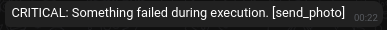
\includegraphics[width=12cm, keepaspectratio]{img/error_send_photo}
    \caption{Mensaje de error enviado cuando el proceso de obtención de la imagen o el envío de esta falla.}
    \label{figura:error send photo}
\end{figure}

Existe, además, el archivo \textit{monitoring.py}, también relativo a este bot de Telegram. Este script se ejecuta en cron tras cada lectura de \textit{datacollecting}. Pretende asegurar que los datos recogidos son coherentes, en caso contrario, envía un mensaje al chat del usuario con el bot indicando el posible error. En \textit{monitoring.py}, solo se contempla que el valor obtenido sea -1, ya que la comprobación de si el dato está en un rango de valores posibles, se realiza a la hora de la recogida. Aunque se podría haber ignorado los datos erróneos, se ha optado por no hacerlo para poder encontrar fácilmente un fallo recurrente de un sensor e incluso poder sacar estadísticas de fallo de dispositivos como se ha especificado en el apartado~\ref{subsec:recogida de datos}.

Como se ha comentado anteriormente, el usuario también recibe mensajes automáticos mediante el bot con información de los actuadores, en concreto, recibe el número de litros usado en la aplicación de riego. Esto se realiza desde la propia aplicación como se comenta posteriormente.

\subsection{Aplicación de riego}
\label{subsec:riego}
En \textit{code/apps/actions} se encuentra el código relativo a los actuadores. En \textit{actions.py} se ha desarrollado una aplicación que sirve para automatizar el riego del sistema. Utiliza el código implementado para la lectura de datos de los sensores para obtener la humedad actual de la tierra. Experimentalmente se ha comprobado que los valores ideales para esta deben estar en torno a 0.25-0.45, esto haría referencia a un 25-45\% de humedad, aproximadamente. Según diversos estudios el porcentaje ideal de humedad de la tierra para el correcto desarrollo de los cultivos se encuentra entre el 25\% y el 50\% en cultivos sensibles a sequía \cite{porcentaje_riego} \cite{humedad_suelo}. Si los valores se saliesen de este rango, podría tener consecuencias negativas para el rendimiento de los cultivos. 

Este script se ejecuta en Cron, midiendo la humedad de la tierra y en función del valor obtenido realiza el riego con mayor o menor cantidad de agua. Si el porcentaje es demasiado bajo utilizará más cantidad y si es cercano a los valores ideales utilizará menos. Esta acción se realiza calculando el tiempo necesario que debe estar encendida la bomba. De nuevo la cantidad de agua que se utiliza se ha obtenido de manera experimental. En general, se ha conseguido mantener la humedad dentro de los parámetros deseados.
Una vez ha realizado el riego satisfactoriamente se envía un mensaje al usuario por Telegram indicando cuantos litros han sido necesarios para realizarlo. Se almacena este dato, además, en la base de datos, en la colección llamada \textit{controllers\_data}.

\begin{figure}[H]
	\centering
    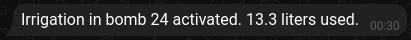
\includegraphics[width=12cm, keepaspectratio]{img/mensaje_riego}
    \caption{Mensaje informativo recibido tras la activación del riego.}
    \label{figura:mensaje riego}
\end{figure} 

Se han contemplado algunos errores potenciales que se tratan como avisos al usuario, por ejemplo, que la diferencia entre dos sensores de humedad que monitorizan la misma zona de riego sea demasiado grande. 
Si dos sensores cercanos ofrecen valores razonablemente distintos, se considera que puede haber ocurrido un error en la medición y se envía una notificación al usuario a través del bot de Telegram.
En el caso de que un cultivo necesite más agua que otro y que ambos estén en la misma zona, esta diferencia puede ser natural. Es por este motivo que no se trata como un error, sino como un \textit{warning}.

\begin{figure}[H]
	\centering
    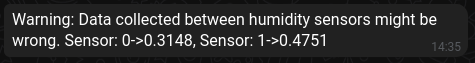
\includegraphics[width=12cm, keepaspectratio]{img/warning_humedad_tierra}
    \caption{Mensaje de posible error enviado cuando la diferencia entre dos sensores de humedad de la tierra es significativa.}
    \label{figura:diferencia de sensores}
\end{figure}

En el directorio \textit{code/apps/actions/controllers} se encuentran el fichero de configuración de actuadores, \textit{config\_controllers.py}. Este fichero es análogo al de los sensores, en el se define la clase \textit{Controller}, como se muestra a continuación:  

\begin{lstlisting}[language=Python]
# Config controllers file
class Controller:
    def __init__(self, pin, data):
        self.pin = pin
        self.data = data # In the bomb case, liters per minute

bomb = Controller(24, 4)
\end{lstlisting}

El propósito de este tipo de ficheros de configuración es el de poder añadir nuevos dispositivos de manera sencilla. 

En este mismo directorio también se encuentra el fichero \textit{controllers.py}, donde se definen las funciones para el apagado y encendido del actuador deseado. Estas funciones reciben el pin de los actuadores. En el caso de la bomba de riego se está utilizando el GPIO 24.

Estas funciones dan de alta el pin de salida deseado haciendo uso de la librería GPIO, con \textit{GPIO.OUT} y luego encienden o apagan el dispositivo que está utilizando pasándole un valor binario.

Al igual que con las funcionalidades descritas anteriormente, la aplicación de riego tiene sus propios logs. Estos logs se encuentran en \textit{code/apps/actions/logs}. En este directorio se encuentran los ficheros \textit{success.log}, \textit{error.log} y \textit{cronerror.log}.
La aplicación se ejecuta en Cron y se lanza una vez al día, a las 00:30.

%%%%%%%%%%%%%%%%%%%%%%%%%%%%%%%%%%%%%%%%%%%%%%%%%%%%%%%%%%%%%%%%%%%%%%%%%%%%%%%%
%%%%%%%%%%%%%%%%%%%%%%%%%%%%%%%%%%%%%%%%%%%%%%%%%%%%%%%%%%%%%%%%%%%%%%%%%%%%%%%%
% CASOS DE USO %
%%%%%%%%%%%%%%%%%%%%%%%%%%%%%%%%%%%%%%%%%%%%%%%%%%%%%%%%%%%%%%%%%%%%%%%%%%%%%%%%

\cleardoublepage
\chapter{Casos de uso}
\label{chap:casos de uso}

En este capítulo se incluyen ejemplos y casos de uso de las funcionalidades introducidas en el capítulo~\ref{chap:diseño e implementación}. Se pretende mostrar ejemplos del flujo de la información, desde que es recogida por los sensores y almacenada en la base de datos, hasta que es visualizada en la aplicación Dash o a través del bot de Telegram.

\section{Ejemplos de uso del sistema}
\label{sec:aplicación de dash ejemplos}
En esta sección se muestran casos de uso y el flujo de funcionamiento de la plataforma completa.
Como norma general que se repite para cada uno de los sensores disponibles, en primer lugar el sensor recoge la información y es guardada en la base de datos. Después, desde la aplicación Dash y desde el Bot de Telegram se puede acceder a la base de datos para visualizar la información. En las siguientes secciones se presentan ejemplos con valores para explicar de mejor manera el proceso.

\subsection{Temperatura y humedad ambiente}
\label{subsec: temperatura y humedad ambiente}
El caso de la temperatura y la humedad ambiente es análogo. En primer lugar se realiza la recogida de datos usando los sensores \textit{DHT22}. Los datos recogidos se suben a la colección \textit{sensors\_data} de la base de datos \textit{greenhouseDB}. En las figuras~\ref{figura:robo3t_ambient_temperature} y ~\ref{figura:robo3t_ambient_humidity} se muestran los datos almacenados de humedad y temperatura ambiente correspondientes al 6 de junio de 2022, para la lectura realizada a las 4 de la mañana. En estas figuras se puede observar la estructura de los documentos que representan la información sobre humedad y temperatura ambiente, que son similares al resto de datos que se manejan en este TFG. El detalle sobre lo que representa cada campo se puede encontrar en la sección~\ref{subsec:arquitectura general}.

\begin{figure}[H]
	\centering
    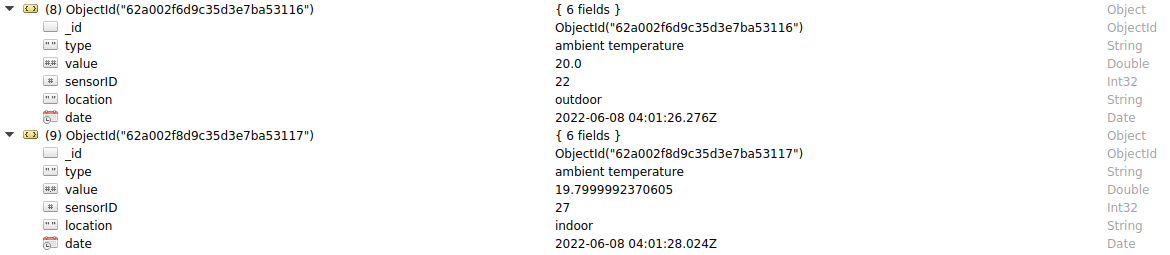
\includegraphics[width=12cm, keepaspectratio]{img/robo3t_ambient_temperature}
    \caption{Datos almacenados en \textit{sensors\_data} para la temperatura ambiente.}
    \label{figura:robo3t_ambient_temperature}
\end{figure}
\begin{figure}[H]
	\centering
    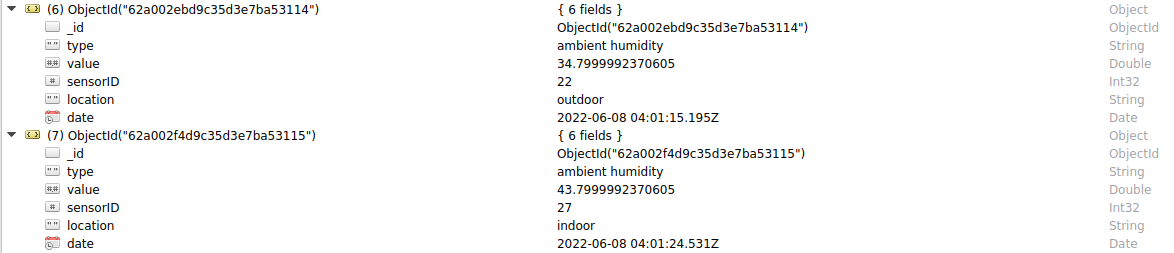
\includegraphics[width=12cm, keepaspectratio]{img/robo3t_ambient_humidity}
    \caption{Datos almacenados en \textit{sensors\_data} para la humedad ambiente.}
    \label{figura:robo3t_ambient_humidity}
\end{figure} 

Una vez la información es almacenada en la base de datos puede ser consultada desde las diferentes aplicaciones que se han desarrollado.
En la figura~\ref{figura:ambient_temperature_01_08_junio} se observa la gráfica obtenida en la aplicación web de Dash que muestra los datos relativos a la temperatura ambiente recogidos desde el 1 hasta el 8 de junio de 2022. Para obtener esta gráfica es necesario acceder al apartado \textit{AMBIENT TEMPERATURE} dentro de \textit{SENSORS DATA} del menú de la aplicación y seleccionar las fechas deseadas en el desplegable de la parte superior derecha diseñado para este uso (ver figura~\ref{figura:desplegable_fecha}). También es posible utilizar los filtros como se explica en la sección~\ref{aplicacion de dash}.

En la figura~\ref{figura:ambient_temperature_01_08_junio} se observa como las lecturas de ambos sensores miden aproximadamente lo mismo, esto confirma el correcto funcionamiento del sistema. En la época del año en la que se realizaron las lecturas el invernadero se encontraba abierto, de manera que la temperatura interior y exterior debe ser similar. Las fluctuaciones que se muestran en la figura se corresponden con las altas temperaturas durante el día y la bajada de estas durante la noche.

\begin{figure}[H]
	\centering
    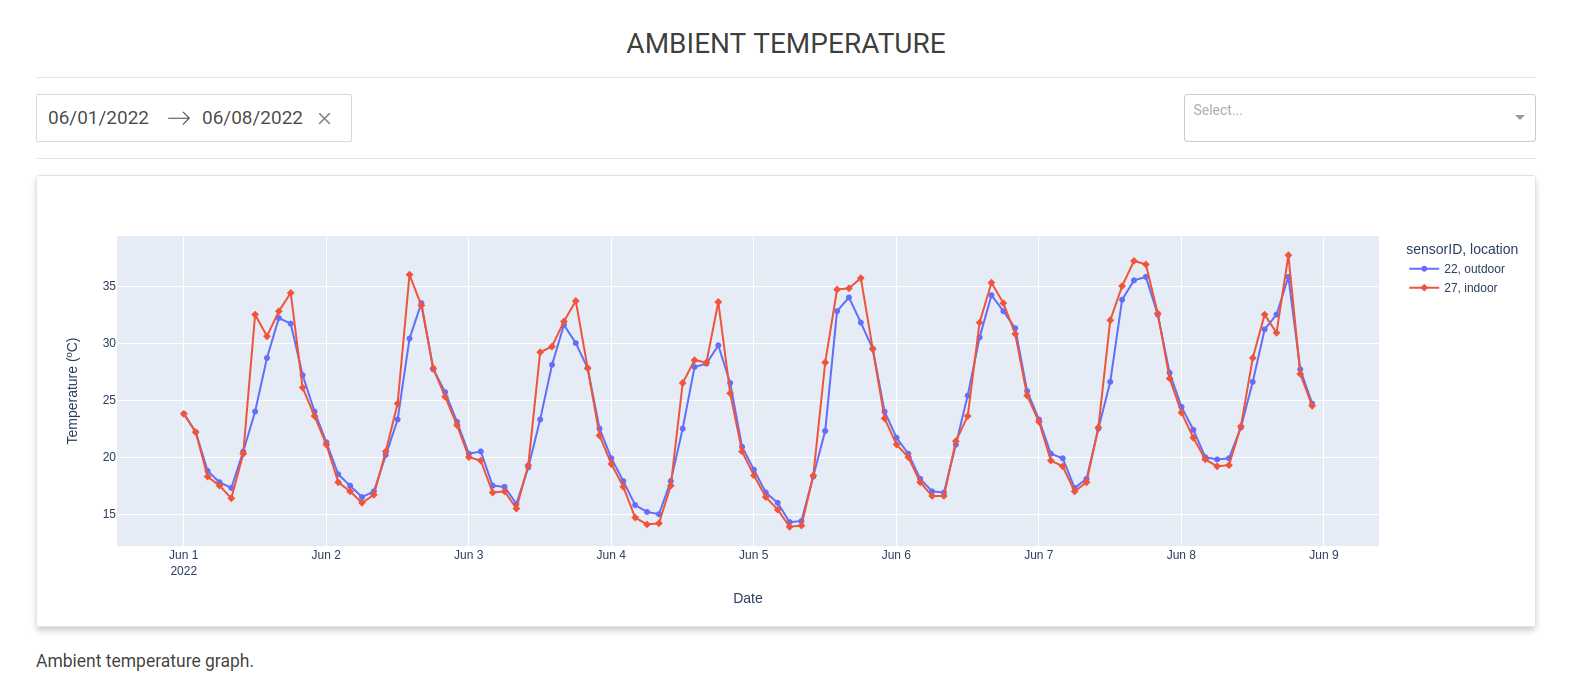
\includegraphics[width=12cm, keepaspectratio]{img/ambient_temperature_01_08_junio}
    \caption{Gráfica obtenida mediante la aplicación web con datos de temperatura ambiente desde 1 al 8 de junio de 2022.}
    \label{figura:ambient_temperature_01_08_junio}
\end{figure}

También es posible obtener esta gráfica haciendo uso del bot de Telegram mediante el comando \textit{/ambienttemperaturefig} con sus parámetros opcionales para indicar la fecha deseada \textit{--startdate} y \textit{--enddate}, como se muestra en la figura~\ref{figura:telegram_ambient_temperature_01_08_junio}.
\begin{figure}[H]
	\centering
    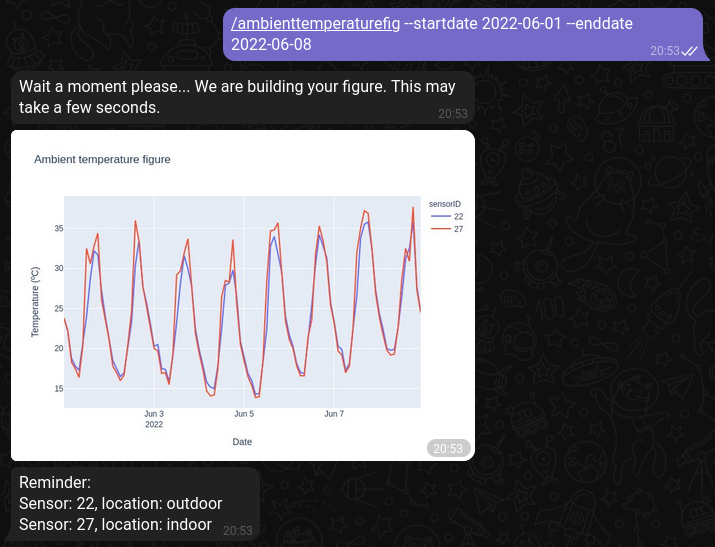
\includegraphics[width=12cm, keepaspectratio]{img/telegram_ambient_temperature_01_08_junio}
    \caption{Gráfica obtenida mediante el bot de Telegram con datos de temperatura ambiente desde 1 al 8 de junio de 2022.}
    \label{figura:telegram_ambient_temperature_01_08_junio}
\end{figure}

Si se ejecuta el comando \textit{/ambienttemperaturefig} sin ningún argumento se obtiene la gráfica con los datos obtenidos por defecto como se muestra en la figura~\ref{figura:ambienttemperaturefig}. Los datos por defecto son los datos de las últimas 24 horas. El comando permite también utilizar únicamente el parámetro \textit{--startdate}(ver figura~\ref{figura:ambienttemperaturefig_startdate}). En el caso de usar únicamente el parámetro \textit{--enddate} se envían los datos desde el primer valor almacenado hasta la fecha de fin indicada, como se muestra en la figura~\ref{figura:ambienttemperaturefig_enddate}. Queda a disposición del usuario el uso de este comando con el parámetro \textit{--enddate}, pero la información que se puede obtener es poca ya que aparecen muchos datos en la misma figura.

\begin{figure}[H]
	\centering
    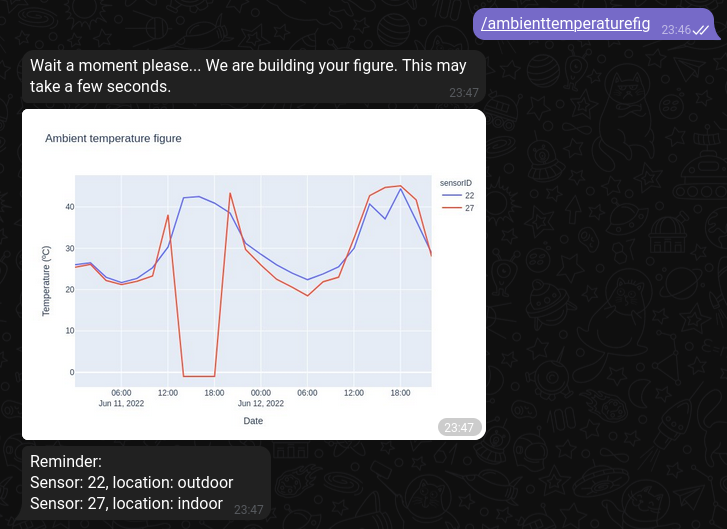
\includegraphics[width=12cm, keepaspectratio]{img/ambienttemperaturefig}
    \caption{Gráfica obtenida mediante el comando \textit{/ambienttemperaturefig} realizado el día 12 de junio de 2022.}
    \label{figura:ambienttemperaturefig}
\end{figure}

\begin{figure}[H]
	\centering
    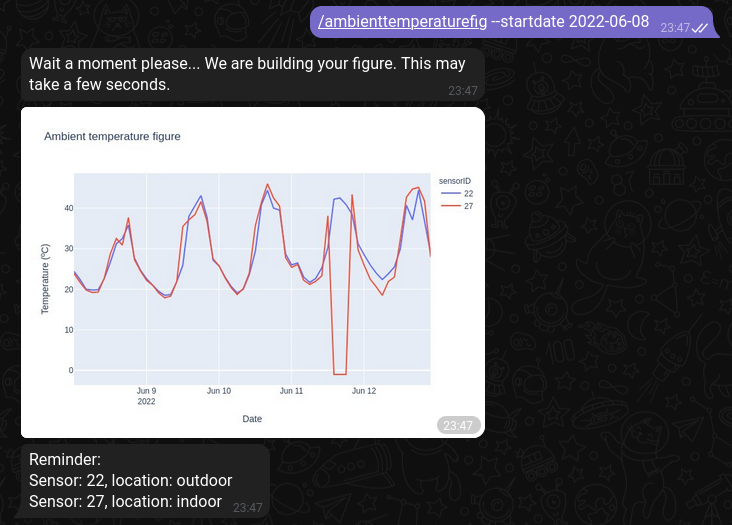
\includegraphics[width=12cm, keepaspectratio]{img/ambienttemperaturefig_startdate}
    \caption{Gráfica obtenida mediante el comando \textit{/ambienttemperaturefig} utilizando el parámetro \textit{--startdate}.}
    \label{figura:ambienttemperaturefig_startdate}
\end{figure}

\begin{figure}[H]
	\centering
    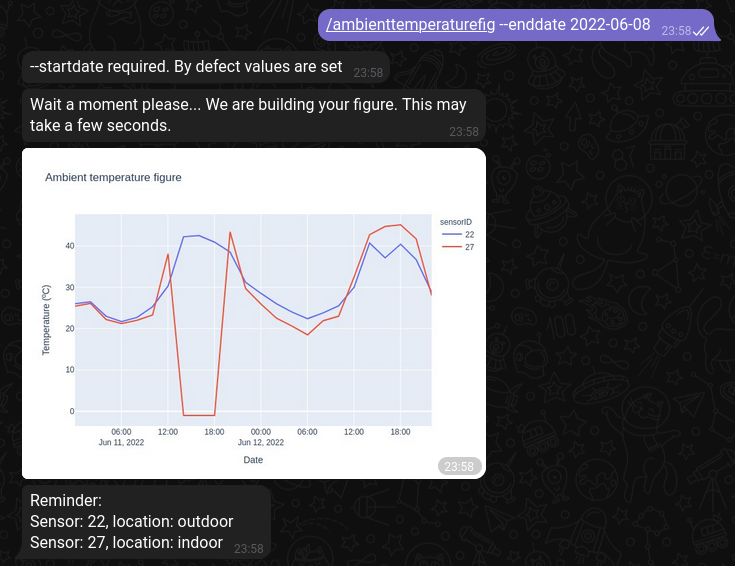
\includegraphics[width=12cm, keepaspectratio]{img/ambienttemperaturefig_enddate}
    \caption{Gráfica obtenida mediante el comando \textit{/ambienttemperaturefig} utilizando el parámetro \textit{--enddate}.}
    \label{figura:ambienttemperaturefig_enddate}
\end{figure}

Como se muestra en las figuras anteriores se puede observar de manera rápida y sencilla un error en la lectura de un sensor, el día 11 de junio de 2022 el sensor 27 de temperatura falló en su lectura. 
Este tipo de errores, tal y como se indica en la sección~\ref{bot de telegram}, también se notifican al usuario de manera que no sea necesario estar consultando el bot para confirmar su correcto funcionamiento. En la siguiente figura se muestra el mensaje recibido tras el error de lectura.
\begin{figure}[H]
	\centering
    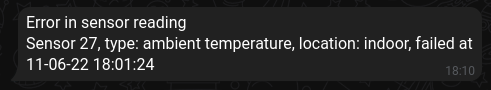
\includegraphics[width=12cm, keepaspectratio]{img/error_sensor_11_junio}
    \caption{Mensaje de error obtenido el 11 de junio de 2022 tras error de lectura de temperatura ambiente del sensor 27.}
    \label{figura:error_sensor_11_junio}
\end{figure}

Otros de los comandos disponibles en el bot de Telegram relativos a la temperatura ambiente son \textit{/ambienttemperature}, con el que se obtiene la temperatura ambiente en tiempo real (ver figura~\ref{figura:ambienttemperature}) y \textit{/ambienttemperaturedb} (ver figura~\ref{figura:ambienttemperaturedb}) que devuelve la última lectura almacenada en la base de datos.
\begin{figure}[H]
	\centering
    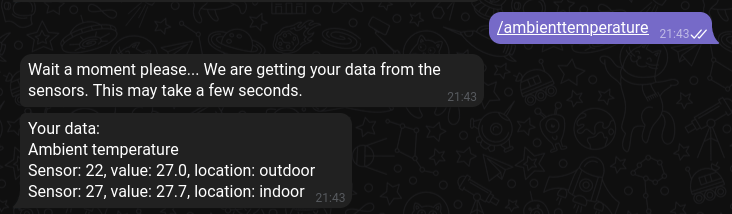
\includegraphics[width=12cm, keepaspectratio]{img/ambienttemperature}
    \caption{Mensaje recibido haciendo uso del comando \textit{/ambienttemperature}.}
    \label{figura:ambienttemperature}
\end{figure}
\begin{figure}[H]
	\centering
    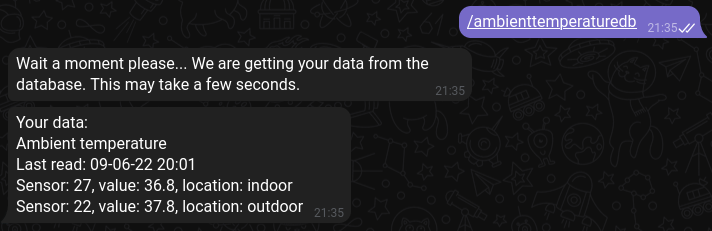
\includegraphics[width=12cm, keepaspectratio]{img/ambienttemperaturedb}
    \caption{Mensaje recibido haciendo uso del comando \textit{/ambienttemperaturedb}.}
    \label{figura:ambienttemperaturedb}
\end{figure}

A pesar de que en los mensajes anteriores se da información sobre los sensores que referencian las figuras y los mensajes, el usuario puede utilizar el comando \textit{/sensorsinfo} para obtener información detallada sobre todos los sensores del sistema como se muestra en la figura~\ref{figura:sensorsinfo}.

\begin{figure}[H]
	\centering
    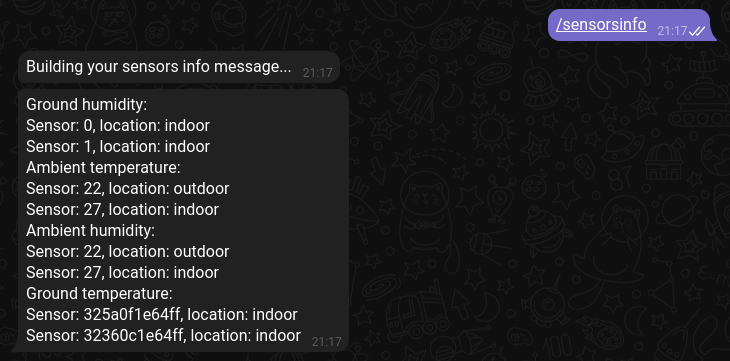
\includegraphics[width=12cm, keepaspectratio]{img/sensorsinfo}
    \caption{Mensaje recibido haciendo uso del comando \textit{/sensorsinfo}.}
    \label{figura:sensorsinfo}
\end{figure}

Como se ha mencionado anteriormente, el caso de la humedad ambiente es análogo al de la temperatura. A continuación se muestran las diferentes figuras relativas a la humedad ambiente. De igual manera, en las figuras se pueden apreciar las fluctuaciones correspondientes al cambio de humedad en la noche respecto al cambio durante el día. Los valores obtenidos por ambos sensores también son similares en sus medidas en cuanto a la humedad.
 
\begin{figure}[H]
	\centering
    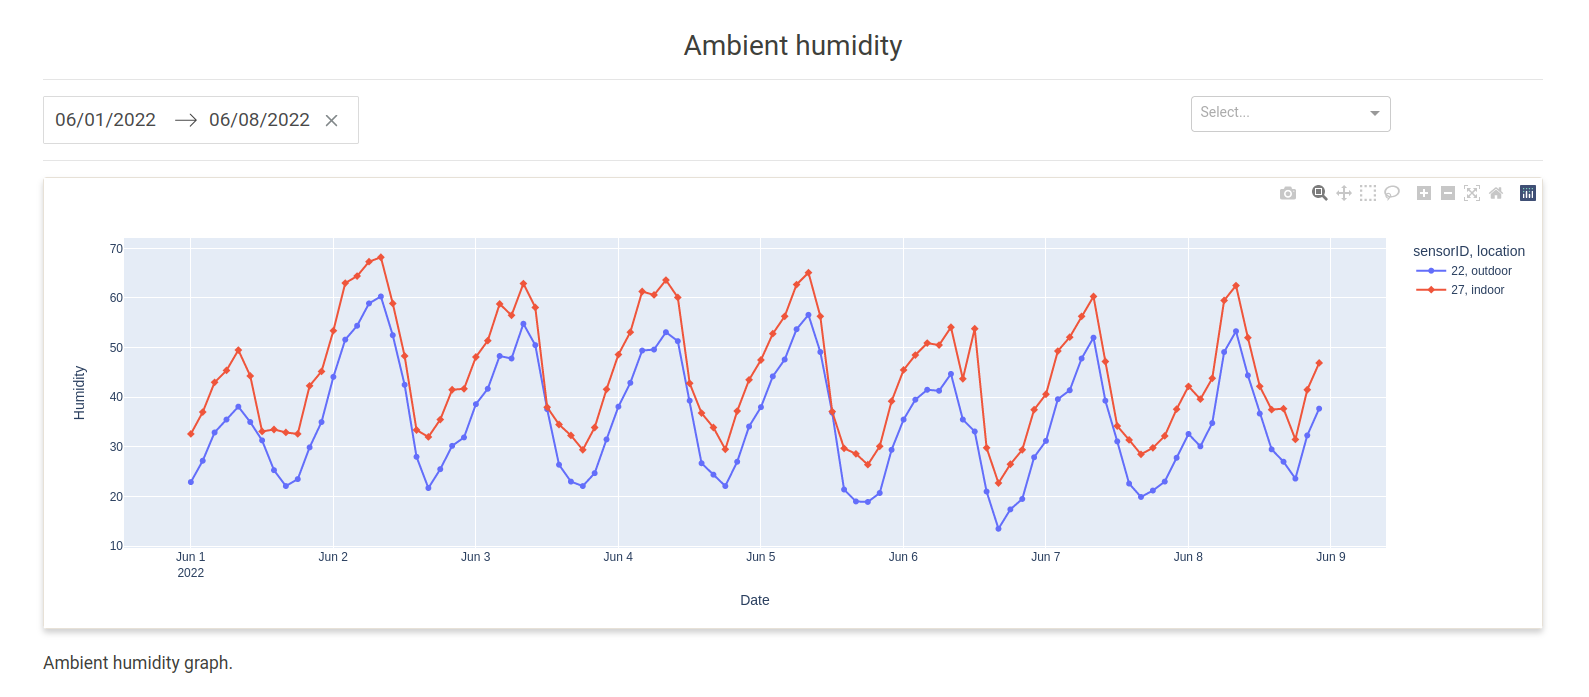
\includegraphics[width=12cm, keepaspectratio]{img/ambient_humidity_01_08_junio}
    \caption{Gráfica obtenida mediante la aplicación web con datos de temperatura ambiente desde 1 al 8 de junio de 2022.}
    \label{figura:ambient_humidity_01_08_junio}
\end{figure}
\begin{figure}[H]
	\centering
    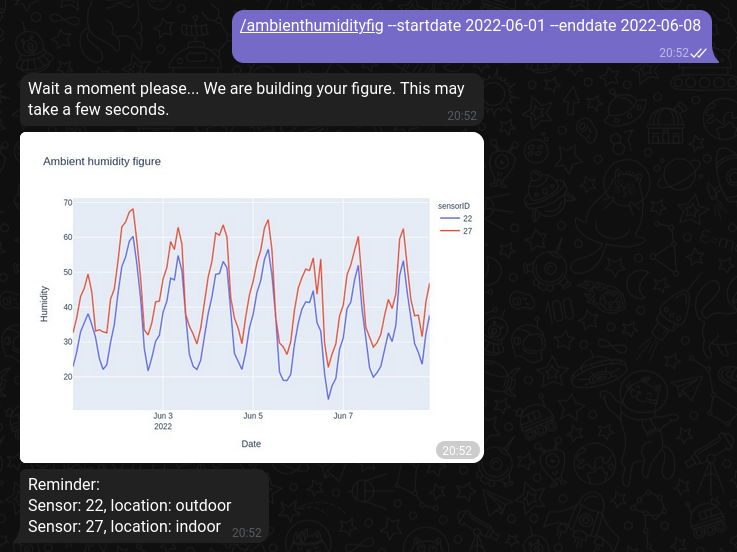
\includegraphics[width=12cm, keepaspectratio]{img/telegram_ambient_humidity_01_08_junio}
    \caption{Gráfica obtenida mediante el bot de Telegram con datos de temperatura ambiente desde 1 al 8 de junio de 2022.}
    \label{figura:telegram_ambient_humidity_01_08_junio}
\end{figure}
\begin{figure}[H]
	\centering
    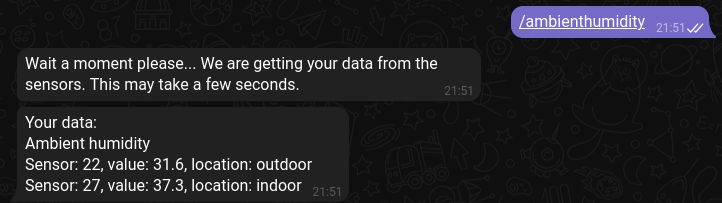
\includegraphics[width=12cm, keepaspectratio]{img/ambienthumidity}
    \caption{Mensaje recibido haciendo uso del comando \textit{/ambienthumidity}.}
    \label{figura:ambienthumidity}
\end{figure}
\begin{figure}[H]
	\centering
    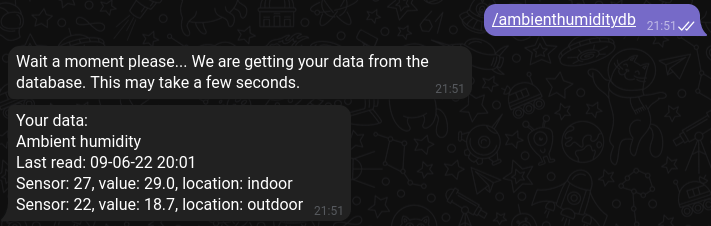
\includegraphics[width=12cm, keepaspectratio]{img/ambienthumiditydb}
    \caption{Mensaje recibido haciendo uso del comando \textit{/ambienthumiditydb}.}
    \label{figura:ambienthumiditydb}
\end{figure}

\subsection{Temperatura de la tierra}
\label{subsec: temperatura de la tierra}
En esta sección se muestra el caso de uso de la aplicación para la recogida y consulta de datos de temperatura de la tierra realiza mediante los sensores \textit{DS18B20}, que son subidos a la colección \textit{sensors\_data} de la base de datos \textit{greenhouseDB}. Es muy similar al descrito en la sección~\ref{subsec: temperatura y humedad ambiente}.
La estructura seguida en la recogida de datos es la que se muestra en la figura~\ref{figura:ground_temperature_robo3t}.

\begin{figure}[H]
	\centering
    \includegraphics[width=12cm, keepaspectratio]{img/ground_temperature_robo3t}
    \caption{Arquitectura de los datos almacenados en \textit{sensors\_data} para la temperatura de la tierra.}
    \label{figura:ground_temperature_robo3t}
\end{figure}
La gráfica en la aplicación web se puede obtener en \textit{GROUND TEMPERATURE} dentro del desplegable \textit{SENSORS DATA} del menú principal como se muestra en la figura~\ref{figura:ground_temperature_dash}. Por defecto, los datos mostrados son los correspondientes a la última semana, al igual que ocurre con el resto de magnitudes en la aplicación web.

\begin{figure}[H]
	\centering
    \includegraphics[width=12cm, keepaspectratio]{img/ground_temperature_dash}
    \caption{Sección \textit{GROUND TEMPERATURE} en la aplicación web de Dash}
    \label{figura:ground_temperature_dash}
\end{figure}


En la figura~\ref{figura:ground_temperature_01_08_junio} se puede observar una diferencia clara en las medidas de las horas centrales del día. Esto se debe a que el sensor representado en azul esta colocado más cercano a la superficie de la tierra, por lo que recibe mucho más calor, sobre todo en días con altas temperaturas como es el caso de la figura. De igual manera se pueden apreciar las fluctuaciones de temperatura correspondientes al día y a la noche.
\begin{figure}[H]
	\centering
    \includegraphics[width=12cm, keepaspectratio]{img/ground_temperature_01_08_junio}
    \caption{Gráfica obtenida mediante la aplicación web de Dash con datos de temperatura de la tierra desde 1 al 8 de junio de 2022}
    \label{figura:ground_temperature_01_08_junio}
\end{figure}

En las sucesivas figuras se muestra el uso del bot de Telegram para obtener los datos relativos a la temperatura de la tierra.

Como se muestra en las figuras~\ref{figura:ground_temperature_telegram} y~\ref{figura:ground_temperature_db_telegram}, la temperatura de la tierra de ambos sensores es bastante pareja en horas que no reciben la luz del sol. Por ejemplo, el comando de la figura~\ref{figura:ground_temperature_telegram} fue ejecutado a las 23:09.

Tal y como se puede observar en la figura~\ref{figura:ground_temperature_diferencias} a medida que avanza el día la diferencia entre las lecturas de ambos sensores es mayor, en cambio, por la noche las mediciones son muy similares.

\begin{figure}[H]
	\centering
    \includegraphics[width=12cm, keepaspectratio]{img/ground_temperature_telegram}
    \caption{Mensaje recibido haciendo uso del comando \textit{/groundtemperature}}
    \label{figura:ground_temperature_telegram}
\end{figure}
\begin{figure}[H]
	\centering
    \includegraphics[width=12cm, keepaspectratio]{img/ground_temperature_db_telegram}
    \caption{Mensaje recibido haciendo uso del comando \textit{/groundtemperaturedb}}
    \label{figura:ground_temperature_db_telegram}
\end{figure}

\begin{figure}[H]
	\centering
    \includegraphics[width=12cm, keepaspectratio]{img/ground_temperature_diferencias}
    \caption{Diferencia entre lecturas de ambos sensores. Medidas tomadas entre las 20 del día 11 de junio de 2022 y las 14 del día 12 de junio de 2022}
    \label{figura:ground_temperature_diferencias}
\end{figure}

Igual que para el resto de magnitudes, es posible utilizar el bot de Telegram para obtener gráficas como se muestra en las figuras~\ref{figura:groundtemperaturefig_telegram} y~\ref{figura:groundtemperaturefig_telegram_options}.

\begin{figure}[H]
	\centering
    \includegraphics[width=12cm, keepaspectratio]{img/groundtemperaturefig_telegram}
    \caption{Gráfica obtenida mediante el comando \textit{/groundtemperaturefig} realizado el día 12 de junio de 2022.}
    \label{figura:groundtemperaturefig_telegram}
\end{figure}

\begin{figure}[H]
	\centering
    \includegraphics[width=12cm, keepaspectratio]{img/groundtemperaturefig_telegram_options}
    \caption{Gráfica obtenida mediante el bot de Telegram con datos de temperatura ambiente desde 1 al 8 de junio de 2022.}
    \label{figura:groundtemperaturefig_telegram_options}
\end{figure}


\subsection{Humedad de la tierra}
\label{subsec: humedad de la tierra}
En esta sección se presenta el tratamiento de la información de la humedad de la tierra. En primer lugar, se realiza la lectura de datos utilizando sensores YL-69. La lectura de estos higrómetros es almacenada en la base de datos \textit{greenhouseDB}, en concreto en la colección \textit{sensors\_data}. La estructura seguida en la recogida de datos de este tipo es la que se muestra en la figura~\ref{figura:arquitectura_humedad_tierra}

\begin{figure}[H]
	\centering
    \includegraphics[width=12cm, keepaspectratio]{img/arquitectura_humedad_tierra}
    \caption{Arquitectura de los datos almacenados en \textit{sensors\_data} para la humedad de la tierra.}
    \label{figura:arquitectura_humedad_tierra}
\end{figure}

Estos datos al igual que en los casos anteriores pueden ser consultados o bien desde la aplicación web, obteniéndola en \textit{GROUND HUMIDITY} dentro del desplegable \textit{SENSORS DATA} del menú principal, o bien desde el bot de Telegram. Todas las figuras, comandos y datos disponibles para la humedad de la tierra son análogos a los casos descritos en las secciones~\ref{subsec: temperatura y humedad ambiente} y~\ref{subsec: temperatura de la tierra}.

La humedad de la tierra está relacionada con la aplicación de riego que se ha desarrollado. Como se expone en la sección~\ref{subsec:riego}. En las figuras sucesivas se muestra como la relación entre los datos de humedad de la tierra y los datos almacenados en la colección \textit{controllers\_data} conservan una estrecha relación.
En las figuras~\ref{figura:figura riego} y~\ref{figura:humedad tierra} se muestra como a mayor sequedad de la tierra el sistema riega con una mayor cantidad de agua. El terreno está más seco cuando la lectura de los sensores es más cercana a uno, es por este motivo que el día 4 de junio se regó con una mayor cantidad de agua que el día 6.

\begin{figure}[H]
	\centering
    \includegraphics[width=12cm, keepaspectratio]{img/figura_riego}
    \caption{Gráfica con datos de riego del 4 al 6 de junio de 2022.}
    \label{figura:figura riego}
\end{figure}

\begin{figure}[H]
	\centering
    \includegraphics[width=12cm, keepaspectratio]{img/ground_humidity}
    \caption{Gráfica con datos de humedad de la tierra del 4 al 6 de junio de 2022.}
    \label{figura:humedad tierra}
\end{figure}

Las gráfica para los actuadores, en este caso las gráfica de riego, se generan siguiendo el mismo proceso que para los sensores. Se puede utilizar la aplicación web, estas figuras se encuentran en el desplegable \textit{IRRIGATION} de la sección \textit{CONTROLLERS DATA} del menú principal (ver figura~\ref{figura:grafica_irrigation_data_04_07_junio}).
Haciendo uso del comando \textit{/irrigationfig}, con sus parámetros opcionales \textit{--startdate} y \textit{--enddate}, se obtiene la figura de riego y con el comando \textit{/irrigationdb} se obtiene el último dato almacenado en la base de datos sobre el riego. El comando \textit{/controllersinfo} devuelve un mensaje con información relevante sobre los diferentes actuadores del sistema, en este caso, sobre la bomba de riego (ver figura~\ref{figura:comando controllers info}).

\begin{figure}[H]
	\centering
    \includegraphics[width=12cm, keepaspectratio]{img/grafica_irrigation_data_04_07_junio}
    \caption{Datos de riego obtenidos mediante la aplicación web del 04 al 07 de junio de 2022.}
    \label{figura:grafica_irrigation_data_04_07_junio}
\end{figure}

\begin{figure}[H]
	\centering
    \includegraphics[width=12cm, keepaspectratio]{img/irrigationfig_04_07_junio}
    \caption{Datos de riego obtenidos mediante el bot de Telegram del 04 al 07 de junio de 2022.}
    \label{figura:irrigationfig_04_07_junio}
\end{figure}

Como se muestra en las figuras~\ref{figura:grafica_irrigation_data_04_07_junio} y~\ref{figura:irrigationfig_04_07_junio} las gráficas elegidas para mostrar los datos relativos al riego son barras que representan la cantidad de litros usados para el riego en un día. En la figura~\ref{figura:comando controllers info} se observa la salida del comando \textit{/controllersinfo}. Este comando proporciona información sobre los actuadores del sistema, en el caso de la bomba se indica su ID (el pin al que está conectado) y su caudal.

\begin{figure}[H]
	\centering
    \includegraphics[width=12cm, keepaspectratio]{img/controllers_info}
    \caption{Salida del comando \textit{/controllersinfo}.}
    \label{figura:comando controllers info}
\end{figure}


\section{Detección de errores e inconsistencias}
\label{sec:detección de errorese inconsistencias}
Como se menciona en el apartado~\ref{aplicacion de dash}, uno de los objetivos de la aplicación web es el de poder realizar un análisis concreto del estado del sistema y encontrar así errores.
La aplicación es útil para detectar comportamientos anómalos en los sensores o actuadores. Por ejemplo, en la figura~\ref{figura:sensor_problemas_higro} se observa que durante varios días el sensor tomaba medidas muy cercanas a 1, esto permitió comprobar que uno de los sensores de humedad del suelo estaba fallando.

\begin{figure}[H]
	\centering
    \includegraphics[width=12cm, keepaspectratio]{img/problemas_sensor}
    \caption{Gráfica que muestra un comportamiento anómalo de uno de los higrómetros.}
    \label{figura:sensor_problemas_higro}
\end{figure}

Otro caso de error se muestra en la figura~\ref{figura:error temperatura ambiente}, donde se muestra que el sensor con ID 22 no estaba funcionando correctamente.

\begin{figure}[H]
	\centering
    \includegraphics[width=12cm, keepaspectratio]{img/ambient_temperature_error}
    \caption{Gráfica que muestra un comportamiento anómalo de uno de los sensores de temperatura ambiente.}
    \label{figura:error temperatura ambiente}
\end{figure}

Otros de los objetivos del control de errores es el de notificar al usuario al momento de su detección. Para ello se envían mensajes cuando esta clase de errores son detectados, como se muestra en los apartados anteriores.

En las secciones~\ref{subsec: temperatura y humedad ambiente}, \ref{subsec: temperatura de la tierra} y \ref{subsec: humedad de la tierra} se muestran las distintas posibilidades que existen para la obtención de información para ese tipo de datos en concreto, pero también es posible realizar este análisis usando los comandos \textit{/sensorsdata}, \textit{/sensorsdatadb} y \textit{/getallfigures}. Con estos comandos se puede obtener datos de todos los tipos de sensores a la vez, en lugar de obtenerlos para cada tipo de sensor individualmente. Sirven para realizar un análisis del estado del sistema más general.

Cuando el bot recibe el comando \textit{/getallfigures} se envían todas las figuras disponibles y un mensaje adicional indicando que ya se ha terminado el proceso (ver figuras~\ref{figura:getallfiguresp1},~\ref{figura:getallfiguresp2} y~\ref{figura:getallfiguresp3}).
 Se observa que todas las figuras tienen lógica con lo comentado en los apartados anteriores y que el sistema se encuentra funcionando correctamente.
 
Las gráficas se generan siguiendo el mismo proceso que el explicado en la sección~\ref{sec:aplicación de dash ejemplos}, sólo que en lugar de ser sobre un grupo de sensores, se generan las gráficas de todos los sensores disponibles.
 
La salida de los comandos \textit{/sensorsdata} y \textit{/sensorsdatadb} que se muestran en las figuras~\ref{figura:sensorsdata} y~\ref{figura:sensorsdatadb} también es coherente.

\begin{figure}[H]
	\centering
    \includegraphics[width=12cm, keepaspectratio]{img/sensorsdata}
    \caption{Salida del comando \textit{/sensorsdata}.}
    \label{figura:sensorsdata}
\end{figure}

\begin{figure}[H]
	\centering
    \includegraphics[width=12cm, keepaspectratio]{img/sensorsdatadb}
    \caption{Salida del comando \textit{/sensorsdatadb}.}
    \label{figura:sensorsdatadb}
\end{figure}

\begin{figure}[H]
  \centering
  \begin{minipage}[b]{0.4\textwidth}
    \includegraphics[width=\textwidth]{img/getallfiguresp1}
    \caption{Primera parte salida del comando \textit{/getallfigures}.}
    \label{figura:getallfiguresp1}
  \end{minipage}
  \hfill
  \begin{minipage}[b]{0.4\textwidth}
    \includegraphics[width=\textwidth]{img/getallfiguresp2}
    \caption{Segunda parte salida del comando \textit{/getallfigures}.}
    \label{figura:getallfiguresp2}
  \end{minipage}
  \hfill
    \begin{minipage}[b]{0.4\textwidth}
    \includegraphics[width=\textwidth]{img/getallfiguresp3}
    \caption{Tercera parte salida del comando \textit{/getallfigures}.}
    \label{figura:getallfiguresp3}
  \end{minipage}
\end{figure}



%%%%%%%%%%%%%%%%%%%%%%%%%%%%%%%%%%%%%%%%%%%%%%%%%%%%%%%%%%%%%%%%%%%%%%%%%%%%%%%%
%%%%%%%%%%%%%%%%%%%%%%%%%%%%%%%%%%%%%%%%%%%%%%%%%%%%%%%%%%%%%%%%%%%%%%%%%%%%%%%%
% CONCLUSIONES %
%%%%%%%%%%%%%%%%%%%%%%%%%%%%%%%%%%%%%%%%%%%%%%%%%%%%%%%%%%%%%%%%%%%%%%%%%%%%%%%%

\cleardoublepage
\chapter{Conclusiones}
\label{chap:conclusiones}
En este capítulo se presentan las conclusiones tras el desarrollo de este TFG. Se indican los objetivos conseguidos y las competencias adquiridas, además de una exposición de los contenidos de distintas asignaturas del grado aplicados a este trabajo.

\section{Consecución de objetivos}
\label{sec:consecución de objetivos}
El objetivo principal propuesto para este TFG era crear un sistema distribuido de monitorización y automatización de un invernadero de bajo coste. Este objetivo, como se indica en el capítulo~\ref{chap:objetivos}, se divide en diversos subobjetivos: montaje del hardware, scripts de recogida y almacenamiento de la información, herramientas de monitorización y visualización y scripts de automatización.

El primer hito consistía en realizar un montaje hardware, montando el invernadero al completo y la electrónica utilizada, en concreto los sensores. Este hito está concretado en las secciones~\ref{sec: montaje físico del invernadero} y~\ref{sec:Arquitectura e implementación hardware}.

El segundo hito consistía en la creación de una serie de scripts para realizar la recogida de información a partir de diferentes sensores y la subida de esta a la base de datos. Este hito ha sido alcanzado con éxito. Como se explica en la sección~\ref{subsec:recogida de datos} estos scripts se ejecutan en Cron y los datos son insertados en la base de datos \textit{greenhouseDB} de MongoDB.

Otro de los subobjetivos marcados era crear una aplicación web para visualizar la información recogida por los sensores. Esto se ha conseguido desarrollando una aplicación web mediante el framework Dash. Toda su funcionalidad queda descrita en la sección~\ref{aplicacion de dash}.
Además del desarrollo de un bot de Telegram que permitiese consultar datos en tiempo real y desde la base de datos. Es posible usar este bot para enviar gráficas con la información de la base de datos y el envío de notificaciones al usuario cuando procediese. La implementación de este bot ha sido llevado a cabo con éxito, desarrollando todas las funcionalidades propuestas mediante el módulo \textit{Telepot} de Python, entre otros. Este desarrollo se indica en la sección~\ref{bot de telegram}.

Por último, se ha automatizado el riego del invernadero utilizando la información proporcionada por los sensores de humedad de la tierra. Se ha conseguido optimizar el riego manteniendo la humedad de la tierra en condiciones ideales para los cultivos, como se explica en la sección~\ref{subsec:riego}.

Un objetivo general era conseguir un sistema de bajo costo y se ha conseguido utilizando sensores y actuadores económicos y herramientas de software gratuitas.

El coste total del proyecto ha sido:

\begin{itemize}
\item \textbf{Invernadero, sacos de cultivo, depósito de agua, tuberías de riego y tierra}: 100€. En este presupuesto no se incluye la compra de semillas o de los cultivos que se vayan a utilizar.
\item \textbf{Caja hermética para electrónica}: 5€
\item \textbf{Raspberry Pi 3B+ y fuente de alimentación}: 45€
\item \textbf{Arduino UNO rev3}: 23€
\item \textbf{Sensores (DHT22, YL-69 y DS18B20)}: 25€
\item \textbf{Actuadores (bomba CESFONJER)}: 15€
\item \textbf{Módulo de relés}: 11€ 
\item \textbf{Resto de componentes electrónicos (cables y Protoboard)}: 20€
\end{itemize}

Estos precios pueden variar ligeramente en función de la disponibilidad y del proveedor. Pero se puede tomar 244€ como un coste total del proyecto orientativo.
Este coste sería para construir todo el sistema desde cero.   


\section{Aplicación de lo aprendido}
\label{sec:aplicación de lo aprendido}
Para la realización de este proyecto, se han aplicado conocimientos adquiridos de diferentes asignaturas cursadas durante el grado:

\begin{itemize}
\item \textbf{Fundamentos de la Programación}: se realiza una introducción a la programación imperativa utilizando como primer lenguaje de programación Pascal.

\item \textbf{Programación de Sistemas de Telecomunicación}: donde se amplían los conocimientos sobre la asignatura anterior, se utiliza el lenguaje de programación Ada para desarrollar software orientado a las comunicaciones, realizando proyectos de mayor complejidad.

\item \textbf{Sistemas y Circuitos}: se imparten los conceptos físicos básicos para realizar una introducción en el análisis y el diseño de circuitos eléctricos.

\item \textbf{Electrónica}: se amplían los conocimientos de la asignatura anterior. Además, se concreta sobre el análisis y diseño de circuitos electrónicos.

\item \textbf{Robótica}: se presentan sensores y actuadores para robots, haciendo hincapié en la programación de estos. Se utiliza el lenguaje de programación Python para abordar los problemas propuestos en la asignatura.

\item \textbf{Sistemas Operativos}: utilizando en lenguaje de programación C se profundiza en el sistema operativo GNU/Linux y sistemas UNIX. Se desarrollan además scripts utilizando Shell Scripting.

\item \textbf{Servicios Telemáticos}: en esta asignatura se utiliza Python como lenguaje de programación para la creación de servicios web. Esta asignatura se centra en el lado del servidor.

\item \textbf{Aplicaciones telemáticas}: se imparten conceptos de desarrollo web, utilizando HTML, CSS y JavaScript.

\item \textbf{Sistemas Distribuidos}: se realiza una introducción a los sistemas distribuidos actuales y se realiza una introducción al diseño de estos.

\item \textbf{Laboratorio de Administración y Gestión de Redes y Sistemas}: se imparte el uso de Docker y técnicas de administración de sistemas. Toda la asignatura se centra en el uso de sistemas de tipo UNIX. Se realiza también una introducción al uso de bots de Telegram para la administración de sistemas.

\item \textbf{Laboratorio de Bases de Datos}: se realiza una introducción al diseño, implementación y mantenimiento de bases de datos.

\end{itemize}
 

\section{Competencias adquiridas}
\label{sec:competencias adquiridas}

Con el desarrollo de este TFG se han ampliado y asentado los conocimientos mencionados en el apartado~\ref{sec:aplicación de lo aprendido}. Además, se han adquirido otros nuevos como son:

\begin{itemize}
\item \textbf{Dash}: el uso de este framework basado en Python y que permite desarrollar aplicaciones web para mostrar datos es una de las competencias adquiridas.

\item \textbf{Bots de Telegram}: a pesar de que en la asignatura \textit{Laboratorio de Administración y Gestión de Redes y Sistemas} se realiza una pequeña introducción, se ha alcanzado un conocimiento mucho mayor sobre el desarrollo de estos para la monitorización y administración de sistemas.

\item \textbf{MongoDB}: en la asignatura \textit{Laboratorio de Bases de Bases de Datos} únicamente se utilizan bases de datos relacionales. Aunque muchos de los conceptos son aplicables a una base de datos orientada a documentos, otra de las competencias adquiridas es el uso de MongoDB.

\item \textbf{Módulos de Python}: la mayoría de los módulos que se han utilizado para el desarrollo de la plataforma no se han enseñado en ninguna de las asignaturas. 

\item \textbf{Mantenimiento y desarrollo de un proyecto de estas características}: a lo largo del grado se han desarrollado proyectos de mayor o menor complejidad, pero nunca uno de estas características y teniendo que realizar su mantenimiento a lo largo del tiempo.

\end{itemize}


\section{Trabajos futuros}
\label{sec:trabajos futuros}

Este trabajo ha sido desarrollado desde cero y algunas de las posibles mejoras de cara a futuro que se podrían implementar son:

\begin{itemize}
\item \textbf{Soporte para nuevos tipos de sensores}. Una de las posibles mejoras sería aumentar el tamaño del sistema añadiendo nuevos tipos de sensores como de CO2 del ambiente o de PH de la tierra.

\item \textbf{Añadir nuevos actuadores al sistema}. Para poder así automatizar otras tareas como abrir y cerrar el invernadero en función de la temperatura y la humedad ambiente.

\item \textbf{Mejora de los componentes}. Al ser un proyecto de bajo coste los componentes son más propensos a errores y tienen una precisión menor.

\item \textbf{Extensión de la aplicación de Dash y del bot de Telegram}. Mejora de estas dos aplicaciones y soporte para los puntos anteriormente descritos. Por ejemplo, que el bot de Telegram notifique cuando hay un error en la ejecución de una de las aplicaciones (\textit{cronerrorlog}), y no únicamente errores de medidas.

\item \textbf{Hacer el sistema completamente autónomo}. Añadiendo una placa solar se puede hacer el sistema autónomo independiente de la corriente eléctrica, de manera que únicamente dependería de la conexión a Internet para la visualización y almacenamiento de datos. La parte de la autonomía del invernadero, dada por los actuadores, seguiría funcionando sin disponer de esta conectividad.
\end{itemize}

%%%%%%%%%%%%%%%%%%%%%%%%%%%%%%%%%%%%%%%%%%%%%%%%%%%%%%%%%%%%%%%%%%%%%%%%%%%%%%%%
%%%%%%%%%%%%%%%%%%%%%%%%%%%%%%%%%%%%%%%%%%%%%%%%%%%%%%%%%%%%%%%%%%%%%%%%%%%%%%%%
% BIBLIOGRAFIA %
%%%%%%%%%%%%%%%%%%%%%%%%%%%%%%%%%%%%%%%%%%%%%%%%%%%%%%%%%%%%%%%%%%%%%%%%%%%%%%%%

\cleardoublepage

\begin{thebibliography}{X}

\bibitem{iot_origen} \textsc{Historia del Internet de las Cosas}
\url{https://www.bbva.ch/en/news/history-of-the-internet-of-things/}

\bibitem{gran_cerebro_tesla} \textsc{Referencias a las palabras de Nikola Tesla sobre la interconectividad futura}
\url{https://medium.com/@fluturads/5-reasons-why-iot-rocks-cf5edfdf49ef}

\bibitem{alan_turing_iot} \textsc{Referencias a las palabras de Alan Turing sobre las capacidades sensoriales}
\url{https://empresas.blogthinkbig.com/breve-historia-de-internet-de-las-cosas-iot/}

\bibitem{arpa_arpanet} \textsc{Origen de ARPA y ARPANET}
\url{https://geekhistory.com/content/why-was-internet-created-1957-sputnik-launches-arpa}

\bibitem{Tim_Berners_Lee} \textsc{Historia de Internet. Tim Berners Lee}
\url{https://webfoundation.org/about/vision/history-of-the-web/}

\bibitem{Kevin_Ashton} \textsc{Cómo Kevin Ashton nombró El Internet de las Cosas}
\url{https://blog.avast.com/es/kevin-ashton-named-the-internet-of-things}

\bibitem{cisco_iot} \textsc{Internet de las Cosas: 75 mil millones de objetos estarán conectados en el mundo en 2025, según informes}
\url{https://www.galileo.edu/trends-innovation/internet-de-las-cosas-75-mil-millones-de-objetos-conectados-en-2025/}

\bibitem{pwa} \textsc{What is a PWA? Progressive Web Apps for Beginners}
\url{https://www.freecodecamp.org/news/what-are-progressive-web-apps/}

\bibitem{nube} \textsc{La industria de la nube no deja de crecer: ya mueve 155.000 millones de euros, un 37 \% más que en 2020}
\url{https://www.xataka.com/empresas-y-economia/industria-nube-no-deja-crecer-mueve-155-000-millones-euros-37-que-2020}

\bibitem{agenda} \textsc{Agenda 2030}
\url{https://www.mitma.gob.es/arquitectura-vivienda-y-suelo/objetivos-desarrollo-sostenible}

\bibitem{papel_agricultura}\textsc{El papel de la agricultura en los objetivos de la agenda 2030}
\url{https://www.iagua.es/blogs/sergio-roman/papel-agricultura-objetivos-agenda-2030}

\bibitem{connected_greenhouses}\textsc{Connected greenhouses: how the Internet of things can feed the planet}
\url{https://hellofuture.orange.com/en/connected-greenhouses-how-the-internet-of-things-can-feed-the-planet/}

\bibitem{alimentos_2050}\textsc{Cómo producir el doble de alimentos en 2050 en un escenario de deterioro de las tierras y sin agua}
\url{https://elpais.com/planeta-futuro/2021-12-14/como-producir-el-doble-de-alimentos-en-2050-en-un-escenario-de-deterioro-de-las-tierras-y-sin-agua.html}

\bibitem{poblacion_mundial}\textsc{La población mundial aumentará en 1.000 millones para 2030}
\url{https://www.un.org/es/desa/world-population-prospects-2017}

\bibitem{agricultura_agua}\textsc{El agua en la agricultura}
\url{https://www.bancomundial.org/es/topic/water-in-agriculture}

\bibitem{agricultura_precision}\textsc{¿Qué es la agricultura de precisión? La gestión digital del campo}
\url{https://www.bbva.com/es/sostenibilidad/que-es-la-agricultura-de-precision-la-gestion-digital-del-campo/}

\bibitem{automated_greenhouse}\textsc{Automated greenhouse}
\url{https://ieeexplore.ieee.org/abstract/document/7295887}

\bibitem{porcentaje_riego}\textsc{Uso de sensores de humedad para definir el riego}
\url{https://www.intagri.com/articulos/agua-riego/uso-de-sensores-de-humedad-para-definir-riego}

\bibitem{humedad_suelo}\textsc{ MODULO 1.4: Determinación de la humedad del suelo}
\url{http://mct.dgf.uchile.cl/AREAS/medio_mod1.4.htm}

\bibitem{adafruit} \textsc{Documentación oficial de Adafruit}
\url{https://learn.adafruit.com}

\bibitem{adafruit} \textsc{Documentación oficial de Pyfirmata}
\url{https://pyfirmata.readthedocs.io/en/latest/}

\bibitem{w1thremsensor} \textsc{Documentación oficial de W1thermsensor}
\url{https://pypi.org/project/w1thermsensor/}

\bibitem{mongodb} \textsc{Documentación oficial de Mongodb}
\url{https://www.mongodb.com/docs/}

\bibitem{pymongo} \textsc{Documentación oficial de Pymongo}
\url{https://pymongo.readthedocs.io/en/stable/}

\bibitem{dash} \textsc{Documentación oficial de Dash}
\url{https://dash.plotly.com/}

\bibitem{plotly} \textsc{Documentación oficial de Plotly}
\url{https://plotly.com/python/}

\bibitem{bootstrap} \textsc{Documentación oficial de Bootstrap}
\url{https://getbootstrap.com/docs/5.2/getting-started/introduction/}

\bibitem{pandas} \textsc{Documentación oficial de Pandas}
\url{https://pandas.pydata.org/docs/user_guide/index.html}

\bibitem{api} \textsc{Documentación oficial para la API de Telegram}
\url{https://core.telegram.org/bots/api}

\bibitem{telepot} \textsc{Documentación oficial de Telepot}
\url{https://telepot.readthedocs.io/en/latest/}
	
\bibitem{heroku} \textsc{Documentación oficial de Heroku}
\url{https://devcenter.heroku.com/categories/reference}
	
\bibitem{docker} \textsc{Documentación oficial de Docker}
\url{https://docs.docker.com/}

\bibitem{latex} \textsc{Platilla de memoria en LaTeX para la ETSIT}
\url{https://github.com/gregoriorobles/plantilla-memoria/blob/master/memoria.tex}

\end{thebibliography}

\end{document}
